\documentclass{sintefbeamer}
\newcommand{\testcolor}[1]{\colorbox{#1}{\textcolor{#1}{test}}~\texttt{#1}}
% meta-data
\titlebackground{images/fondo}


\title{``Acondicionamiento acústico de salas de reuniones y sala de ensayo, Campus Los Canelos, UACh" }
\subtitle{Proyecto de acondicionamiento acústico - ACUS213}
\author{\href{daniela.narvaez01@alumnos.uach.cl}{Daniela Narváez E.} \newline \href{rafael.penailillo@alumnos.uach.cl}{Rafael Hayde P.}}
\date{\today}

% No borrar latexmkrc, debido a que es el archivo que deja la fecha y hora de Chile

\captionsetup{belowskip=0.7pt,aboveskip=0.6pt}
\begin{document}

\maketitle

\section{Introducción}
\begin{frame}{\thesection \, \secname}
La importancia del acondicionamiento acústico radica en su capacidad para mejorar la experiencia auditiva de las personas que utilizan estos espacios. En el caso de las salas de reuniones, es imprescindible una óptima inteligibilidad de la palabra ya que la comprensión del mensaje oral es de suma importancia (Carrión Isbert, 1990). 

En el contexto de una sala de ensayo de orquesta, el acondicionamiento acústico es crucial para lograr una reproducción fiel y equilibrada de los instrumentos musicales, permitiendo a los músicos escucharse entre sí y trabajar en conjunto de manera óptima.
\end{frame}

\begin{frame}{Objetivos}
\begin{itemize}
    \item \textbf{Objetivo General:} \\
    Proponer un acondicionamiento acústico para dos salas de reuniones y una sala de ensayo de orquesta, en el Centro de Extensión Campus los Canelos, UACh.

    \item \textbf{Objetivos Específicos:}
    \begin{itemize}
        \item Caracterizar acústicamente las salas.
        \item Analizar los parámetros acústicos de las salas.
        \item Generar una propuesta de diseño de acondicionamiento acústico para optimizar el sonido de las salas.
        \item Comparar los resultados mediante recomendaciones internacionales. 
        \item Elaborar un presupuesto del acondicionamiento acústico para cada sala.

    \end{itemize}
\end{itemize}
\end{frame}
\section{Antecedentes}
\begin{frame}{Geolocalización}
    \begin{figure}
        \centering
        \includegraphics[width=8cm]{images/Geolocalización.png}
        \caption{Geolocalización del lugar}
        \label{fig: geolocalización}
    \end{figure}
\end{frame}
\begin{frame}{Salones}
    \begin{figure}[!htb]
\minipage{0.35\textwidth}
  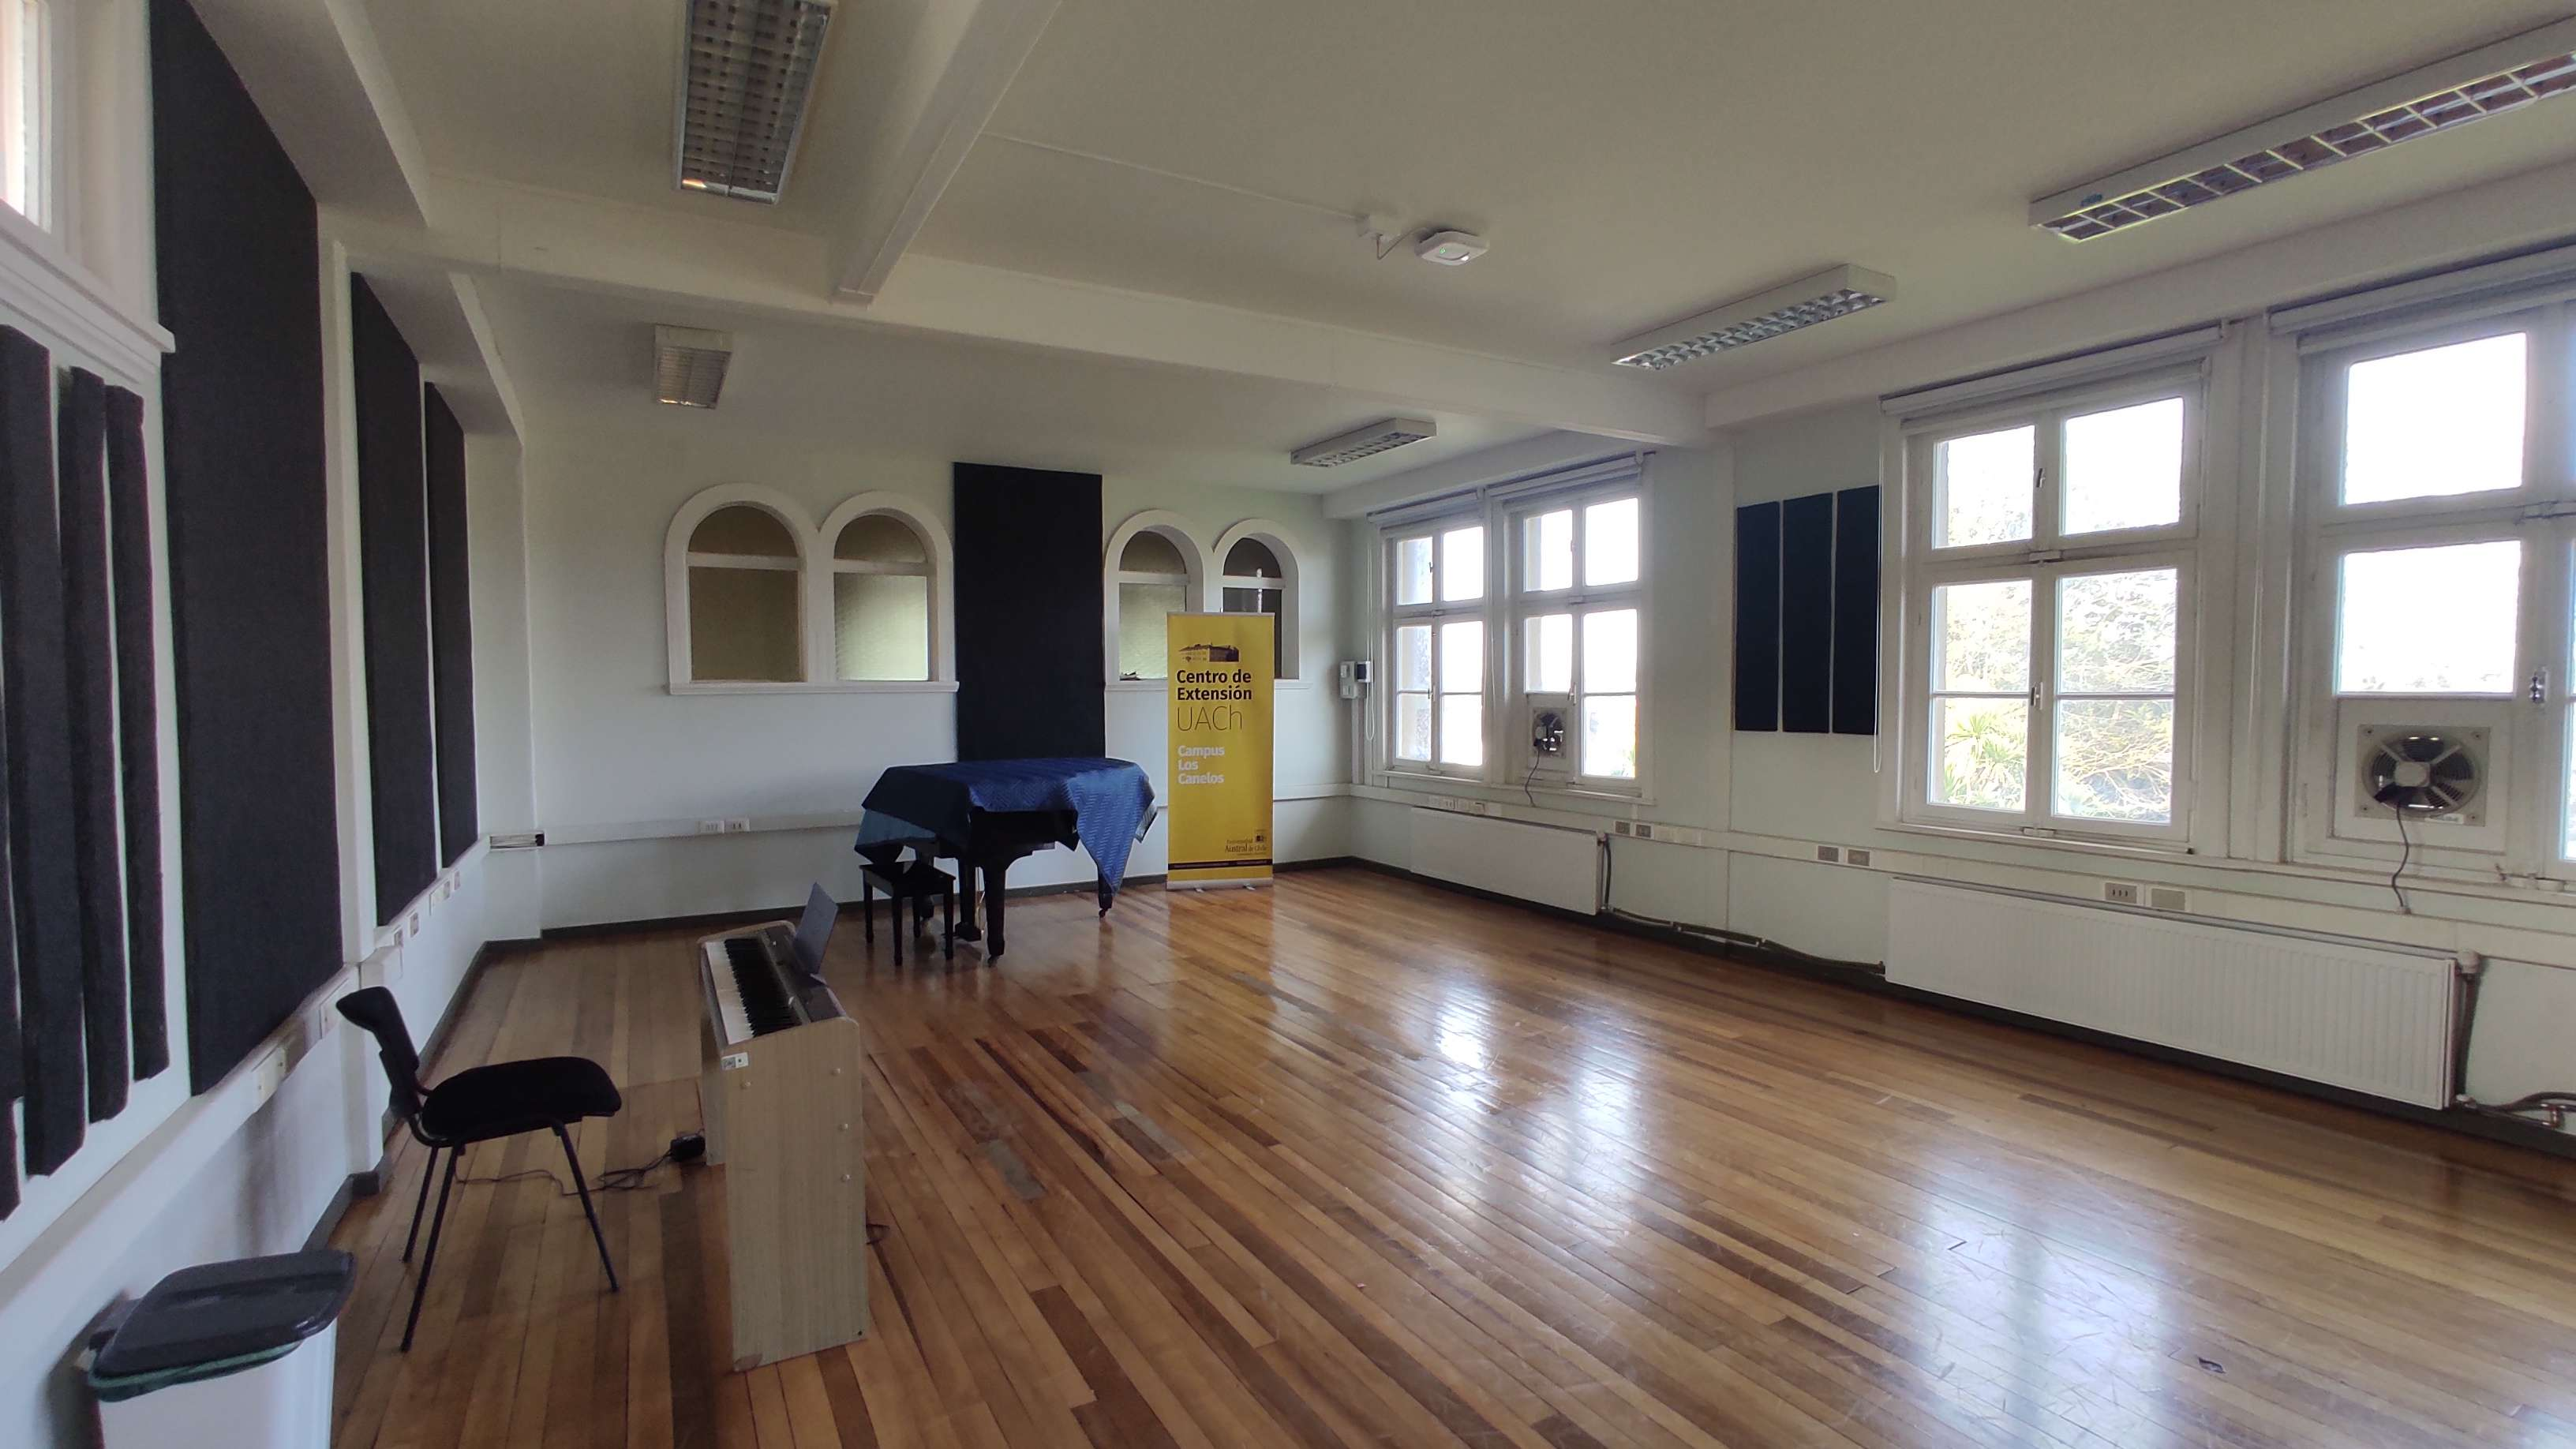
\includegraphics[width=\linewidth]{images/Fotos recinto/Sala OCV.jpg}
  \caption{Sala de ensayo OCV.}\label{fig:sala-ensayo}
\endminipage\hfill
\minipage{0.35\textwidth}
  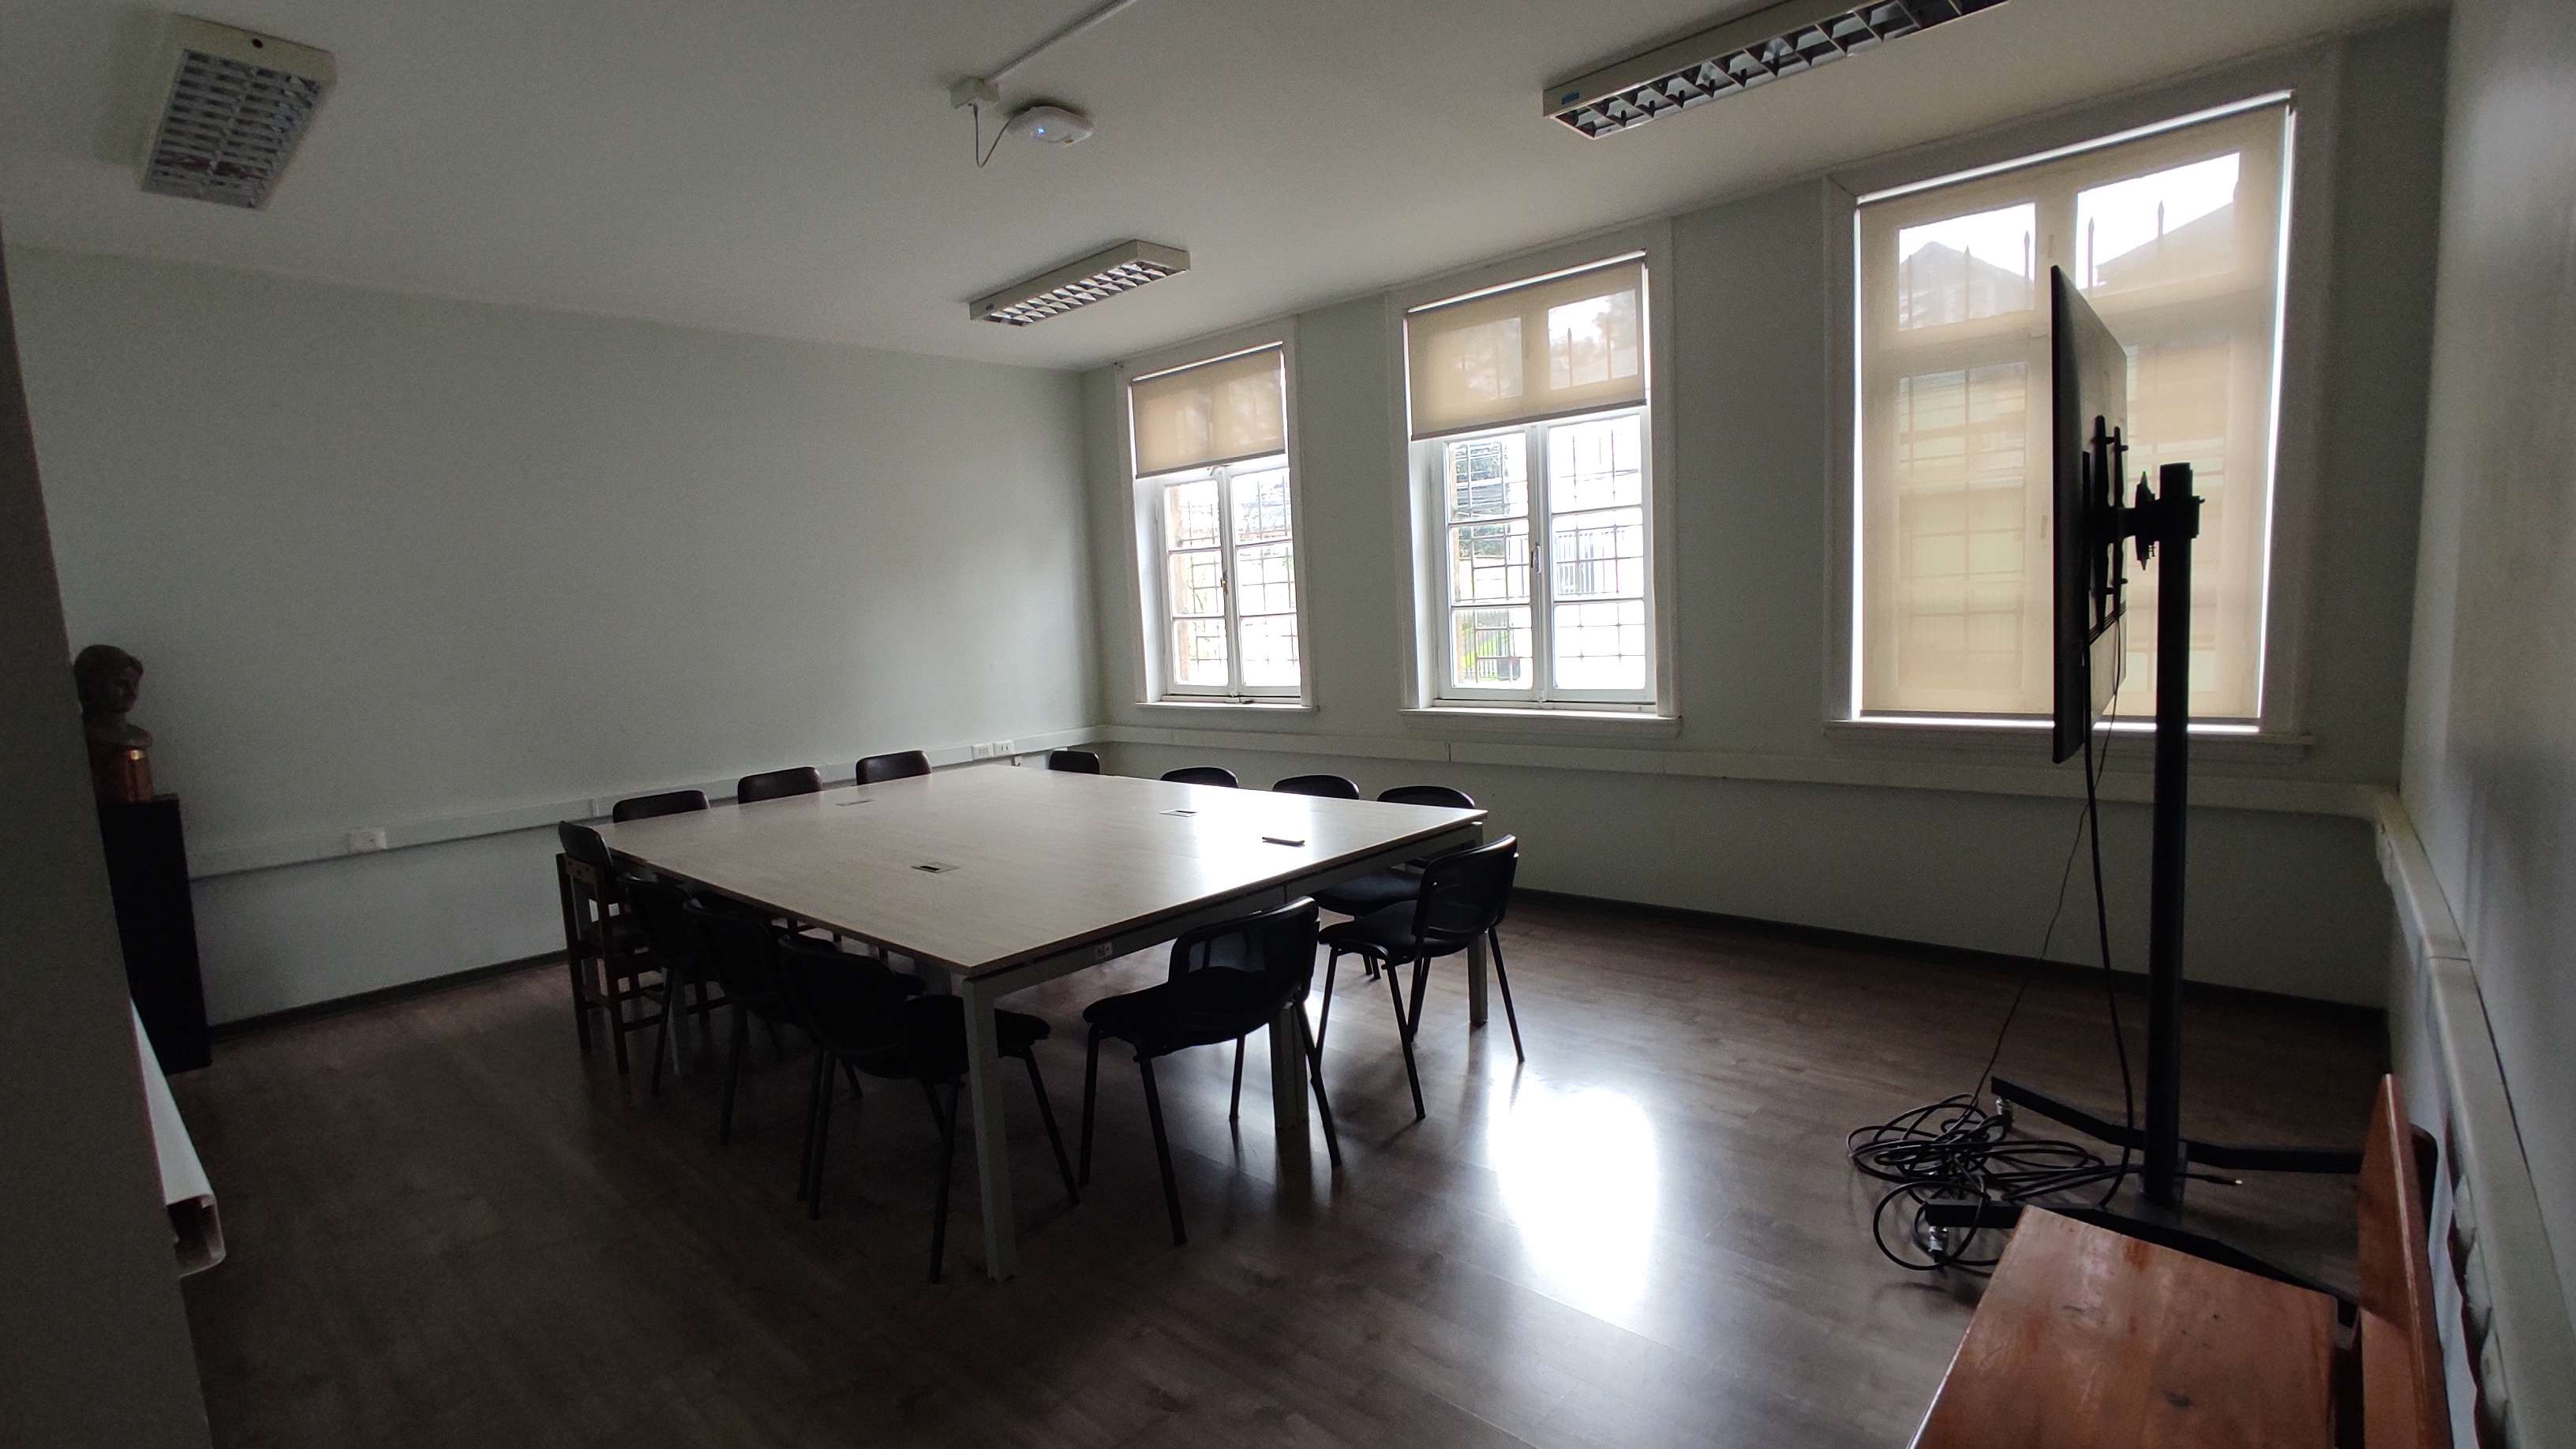
\includegraphics[width=\linewidth]{images/Fotos recinto/Sala 1.jpg}
  \caption{Sala de reunión 1.}\label{fig:sala-reunion1}
\endminipage\hfill
\minipage{0.35\textwidth}%
  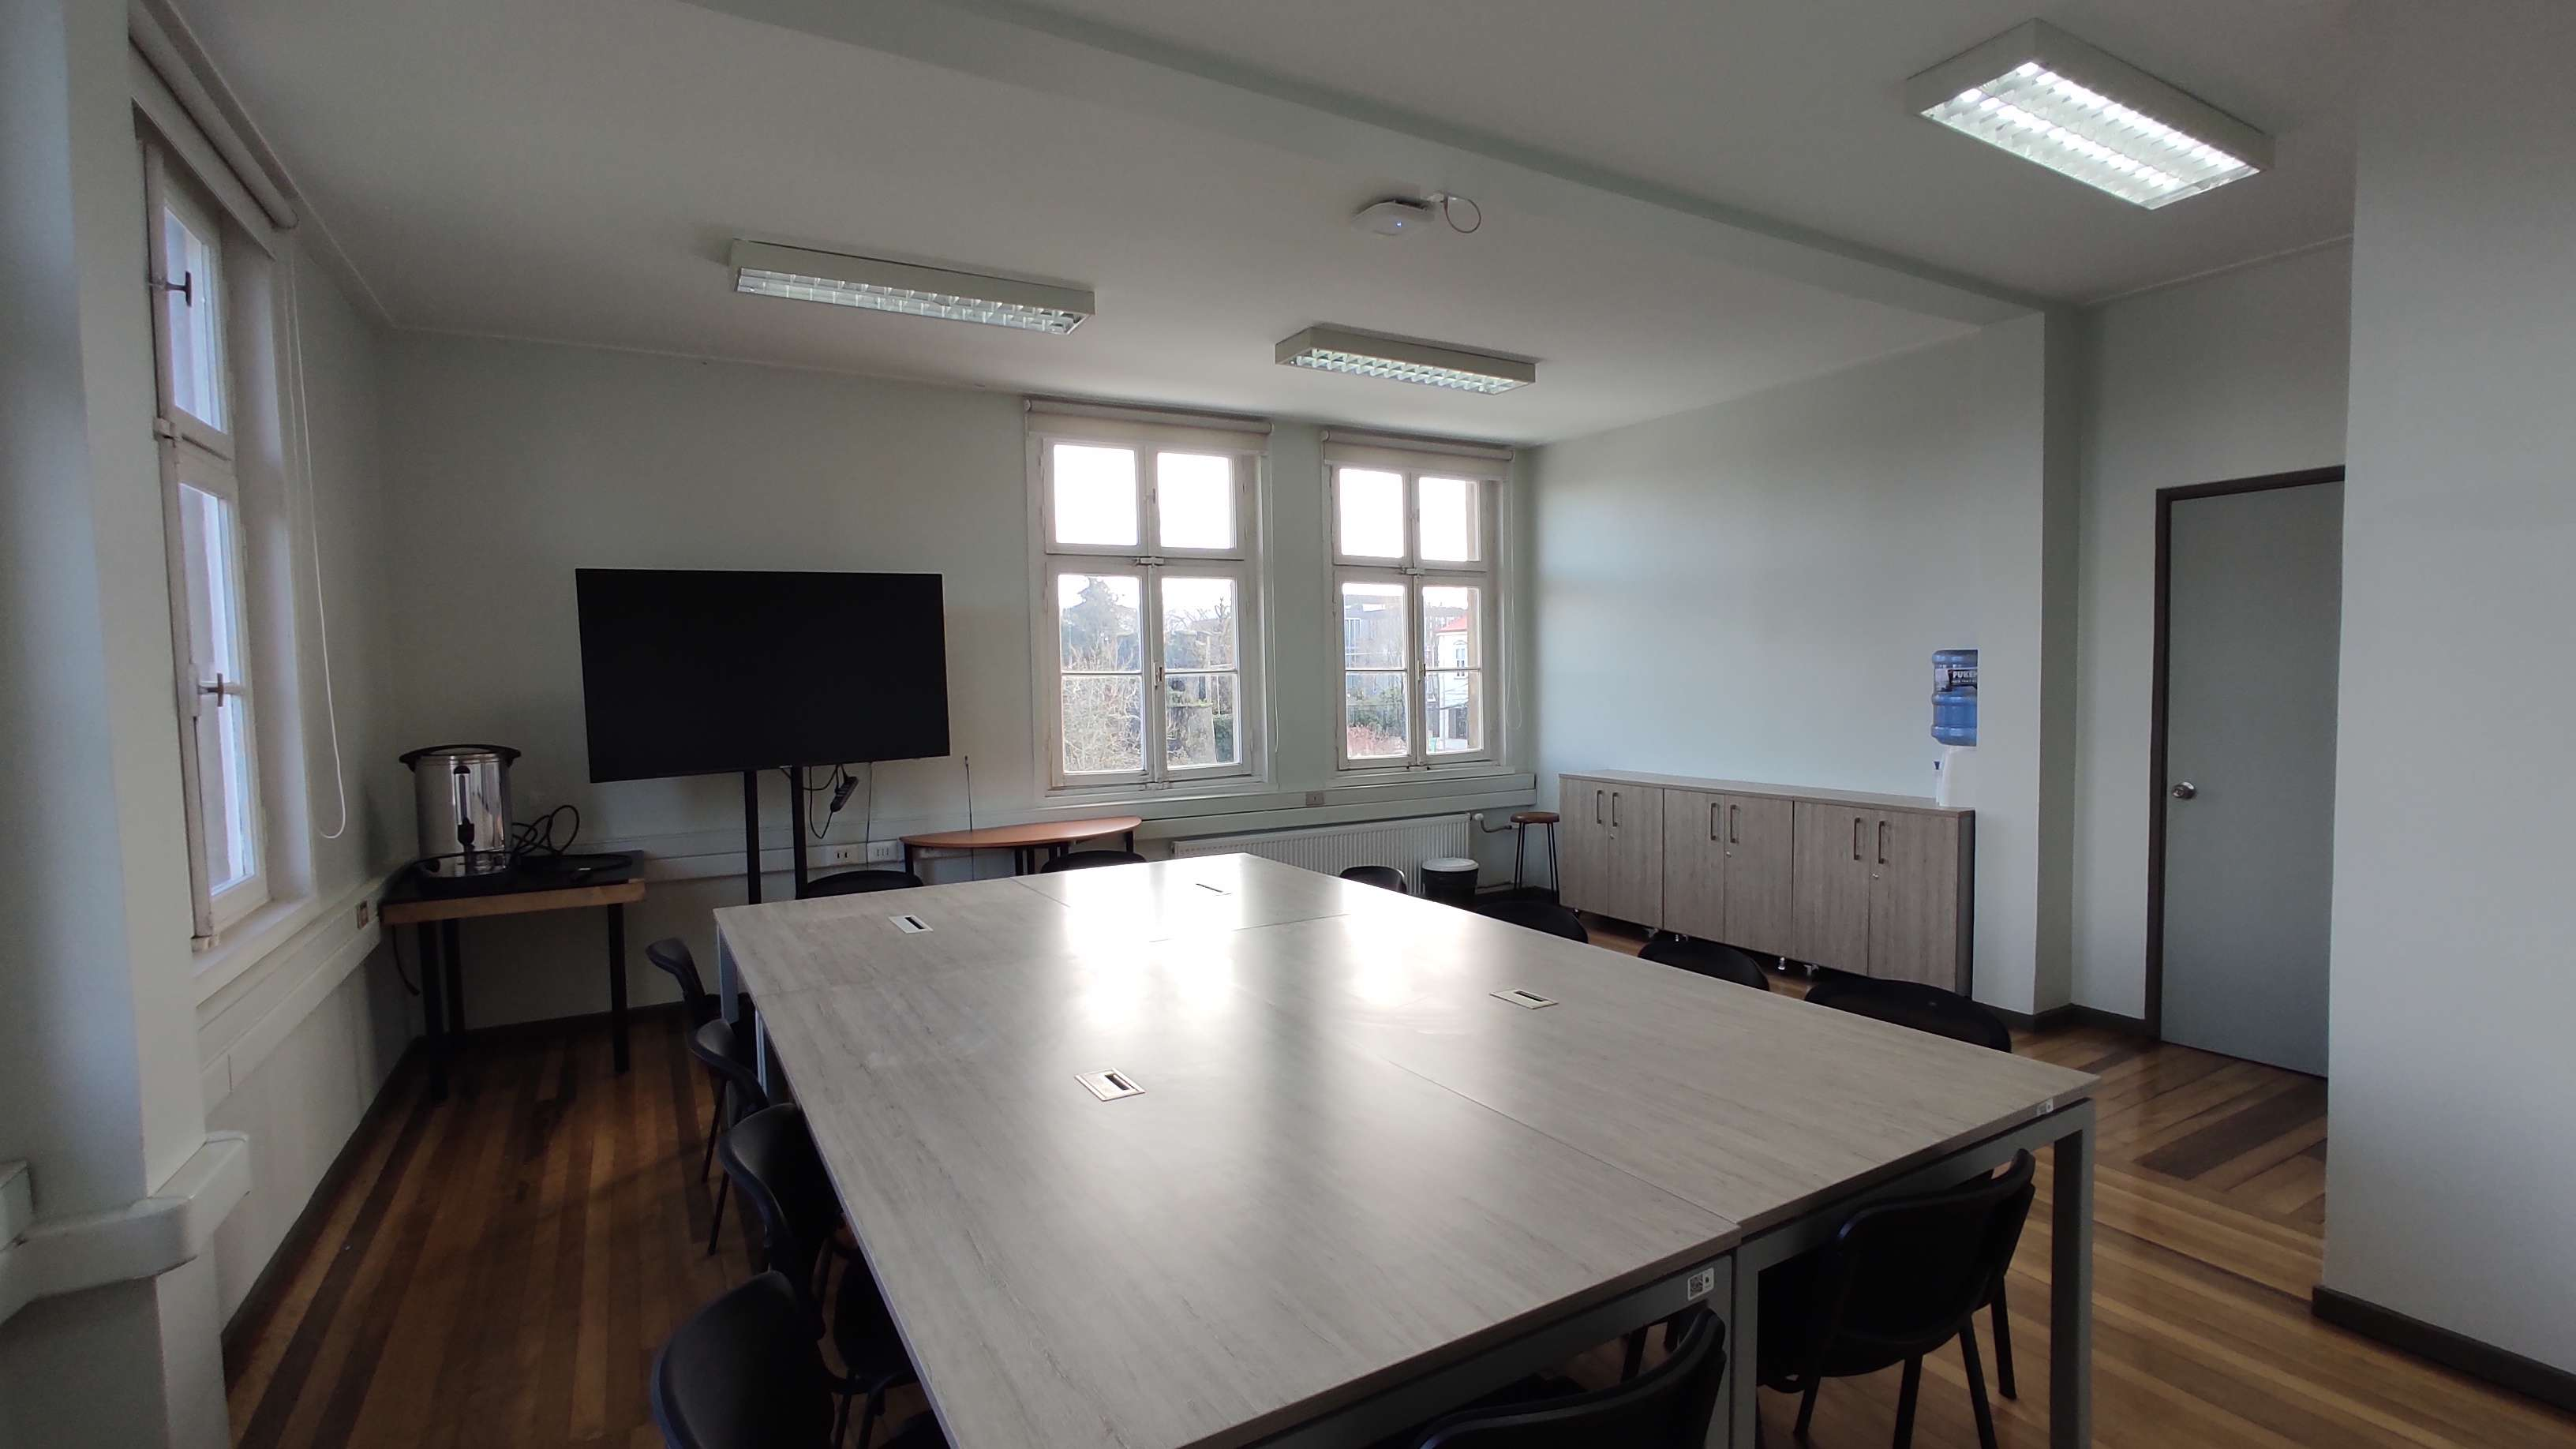
\includegraphics[width=\linewidth]{images/Fotos recinto/Sala 2.jpg}
  \caption{Sala de reunión 2.}\label{fig:sala-reunion2}
\endminipage
\end{figure}
\end{frame}
\begin{frame}{Salones}
El volumen de cada recinto se ven en la siguiente tabla
    \begin{table}[H]
        \centering
        \caption{Volumen de salas}
        \label{tab:volumne de salas}
        \begin{tabular}{|l|c|}
        \hline
         \textbf{Salón} & \textbf{Volumen $m^3$} \\ \hline
         Sala de ensayo & 179 \\ \hline
         Sala de reunión 1 & 115 \\ \hline
         Sala de reunión 2 & 101 \\ \hline
        \end{tabular}
    \end{table}
\end{frame}
\section{Planificación}

\begin{frame}{Cronograma}
Esta planificación se plantea por semanas, desde la semana del 21 de agosto hasta la semana del 2 de diciembre del presente año. 
\begin{figure}
    \centering
    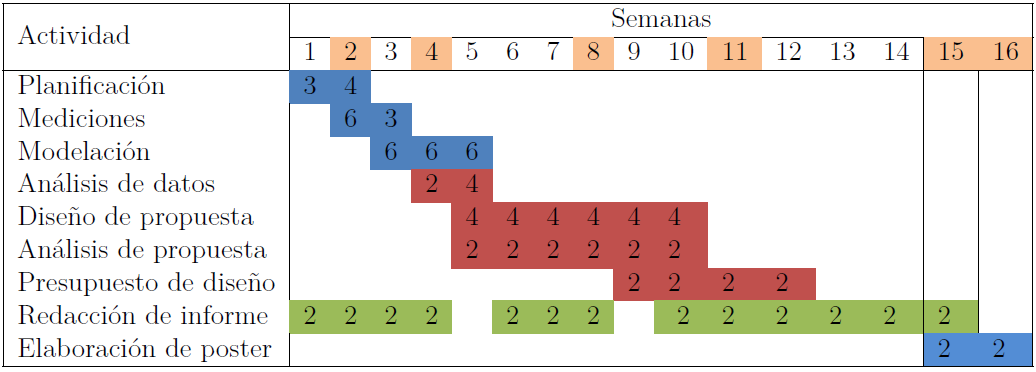
\includegraphics[width=\textwidth]{images/CartaGantt}
    \caption{Carta Gantt del proyecto}
    \label{fig:carta gantt}
\end{figure}

\end{frame}

\section{Metodología}

\begin{frame}{Medición de dimensiones de los recintos}
\begin{figure}
    \centering
    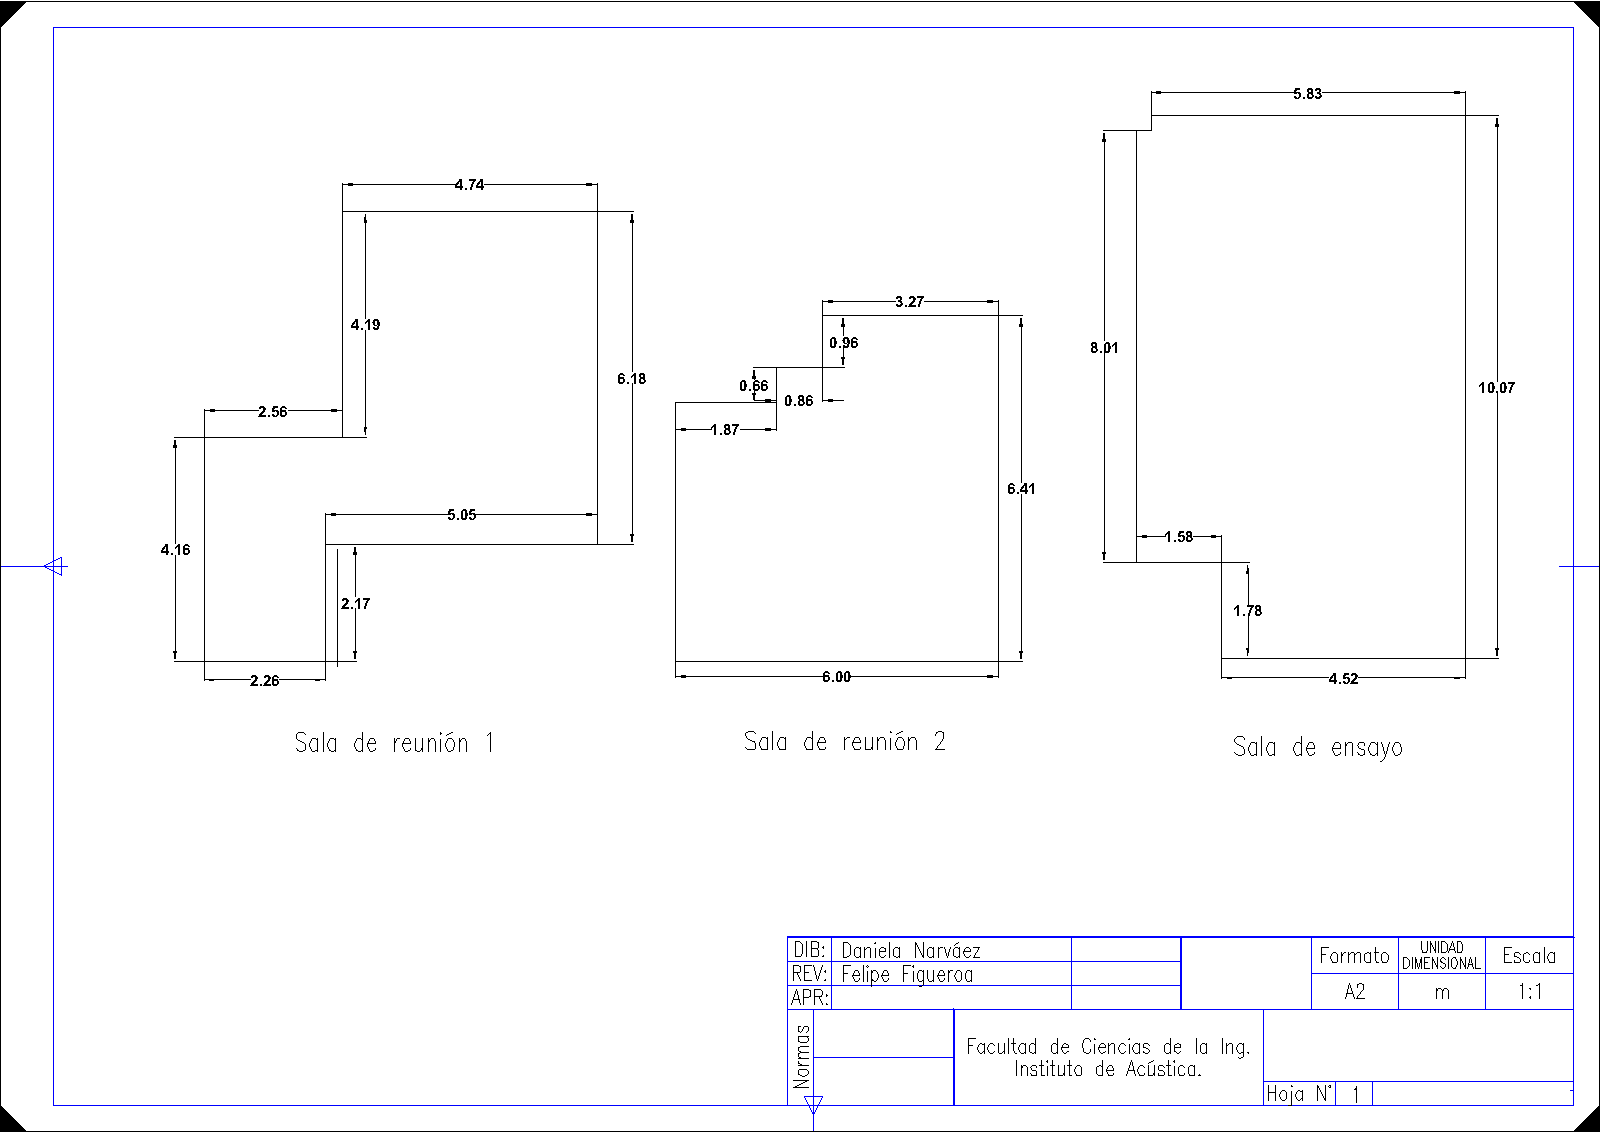
\includegraphics[scale=0.2]{images/Planos/Planos.png}
    \caption{Planos de salas}
    \label{fig: planos}
\end{figure}
\end{frame}
\begin{frame}{Medición de ruido de fondo}
    Para poder caracterizar acústicamente los salones se realizaron mediciones de ruido de fondo y tiempo de reverberación.
    %insertar imágenes de mediciones
    \begin{figure}[H]
        \centering
        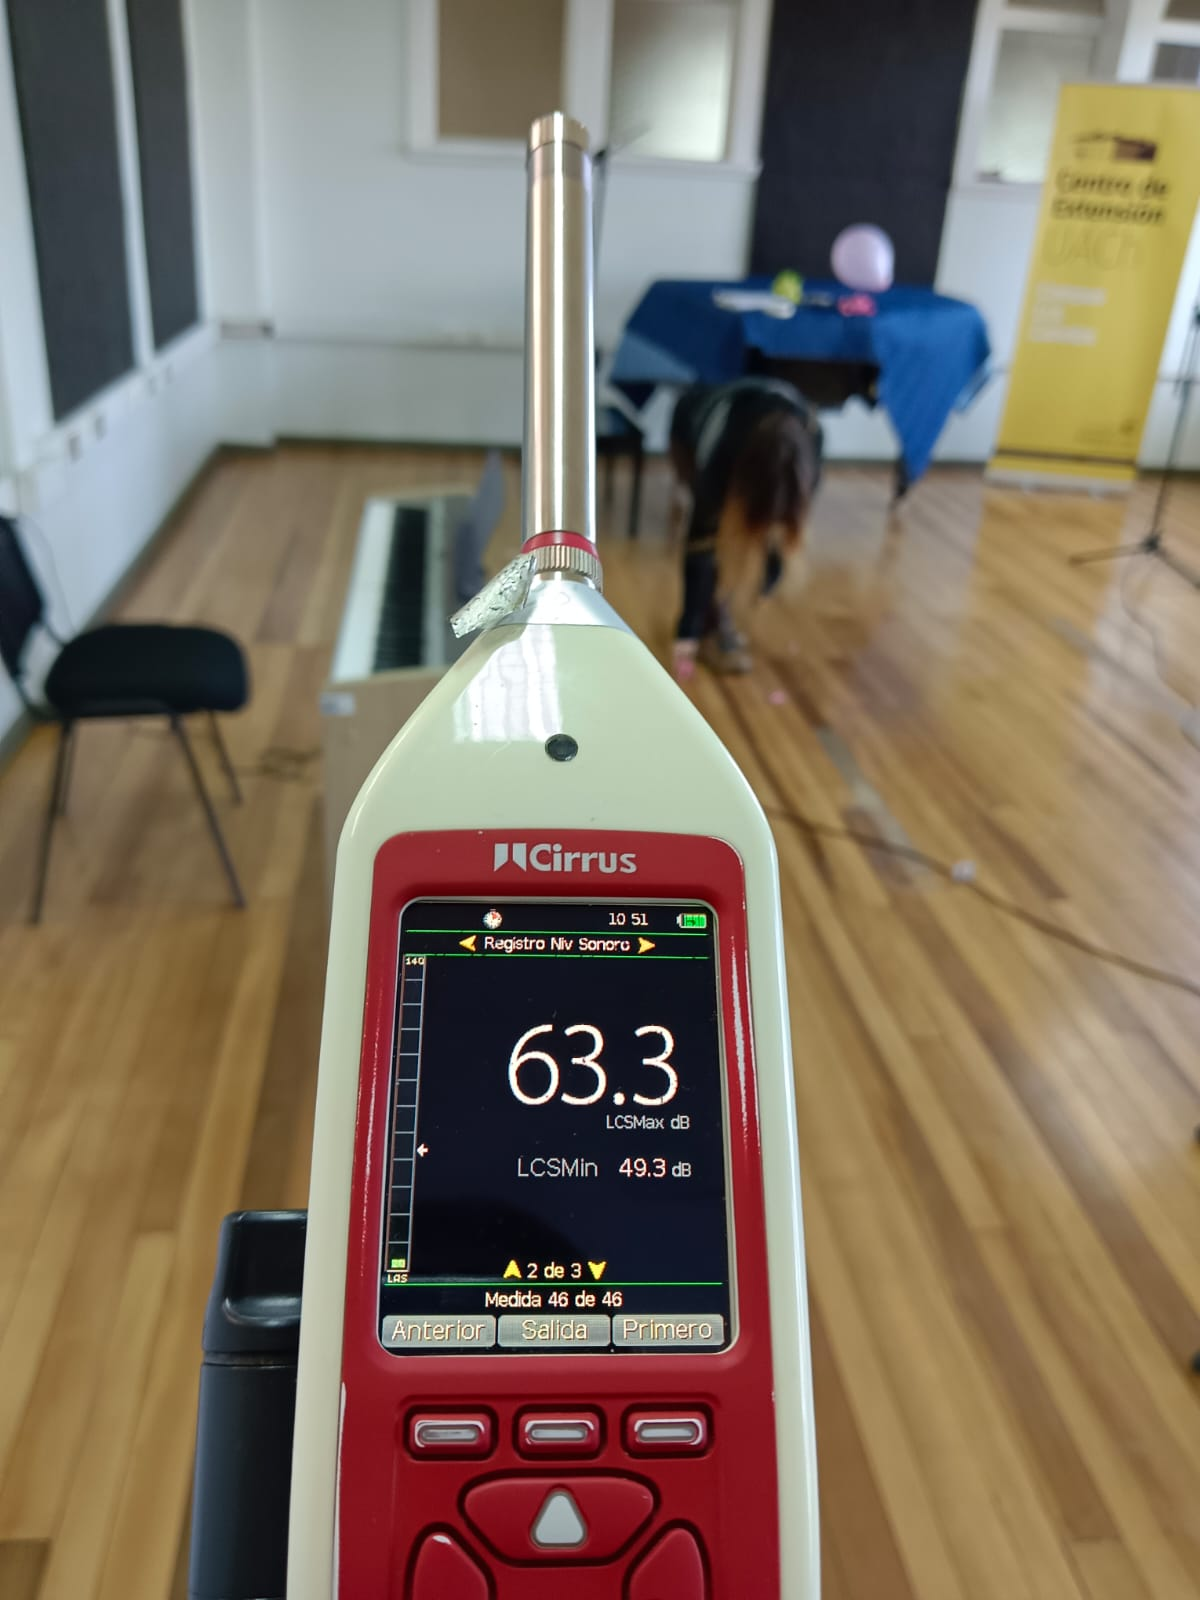
\includegraphics[width=4cm]{images/Fotos Mediciones/medicionRDF.jpeg}
        \caption{Medición de ruido de fondo}
        \label{fig: medicion de rdf}
    \end{figure}
\end{frame}
\begin{frame}{Medición de tiempo de reverberación}
    \begin{figure}[H]
        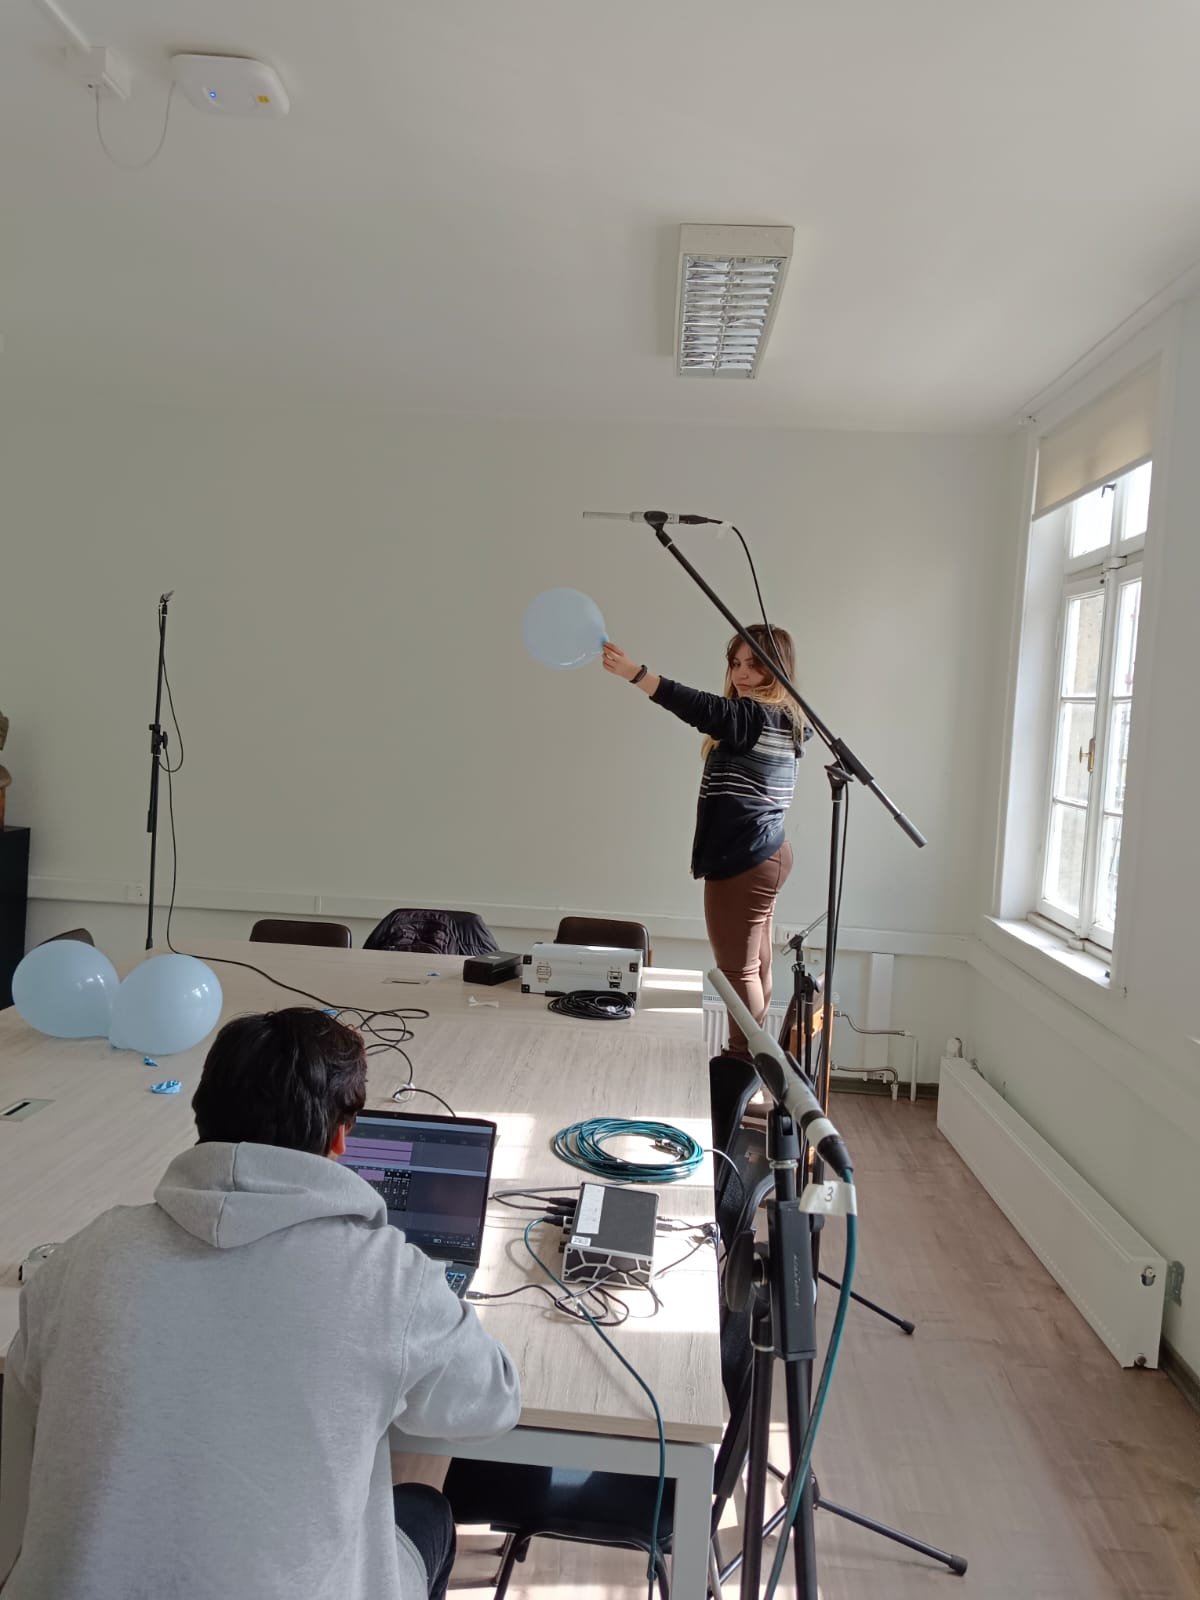
\includegraphics[width=4cm]{images/Fotos Mediciones/medicionRT.jpeg}
        \caption{Medición de tiempo de reverberación}
        \label{fig: medicion rt}
    \end{figure}
\end{frame}
% \begin{frame}{Medición de parámetros acústicos de los recintos}
% Para poder caracterizar acústicamente los salones se utilizaron los siguientes instrumentos:
% \begin{table}[H]
%     \centering
%     \caption{Instrumentación utilizada para las mediciones}
%     \label{tab:instrumentacion}
%     \resizebox{\textwidth}{!}{%
%     \begin{tabular}{|l|l|}
%     \hline
%     \textbf{Instrumentos} & \textbf{Uso}\\ \hline
%     Sonómetro Cirrus CR:$171$B & Medir nivel de presión sonora equivalente \\ \hline
%     Micrófono Behringer ECM$8000$ & Recibir el nivel de las fuentes\\\hline
%     Conectores XLR & Enviar señal de audio\\ \hline
%     Interfaz de audio TASCAM US $4$x$4$ & Procesar señales de audio\\ \hline
%     Cinta métrica & Medir distancia de fuente y micrófonos \\ \hline
%     Termómetro e higrómetro digital & Medir temperatura y humedad en el lugar de medición\\ \hline
%     Protectores auditivos & Proteger oídos de la exposición de sonidos fuertes  \\ \hline
%     Notebook con software ARTA & Procesar y analizar señales   \\ \hline
%     Globos & Fuente impulsiva \\ \hline
%     \end{tabular}
%     }
% \end{table}    
% \end{frame}

% \begin{frame}{Ruido de fondo}
% Para medir el ruido de fondo se utilizó el sonómetro Cirrus midiendo 5 minutos, hasta que el nivel de presión sonora equivalente se estabilice, basándose en el procedimiento descrito en el D.S. $38/11$
% \end{frame}

% \begin{frame}{Tiempo de reverberación}
%  ISO $3382$-$2$
%  \begin{figure}
%     \centering
%     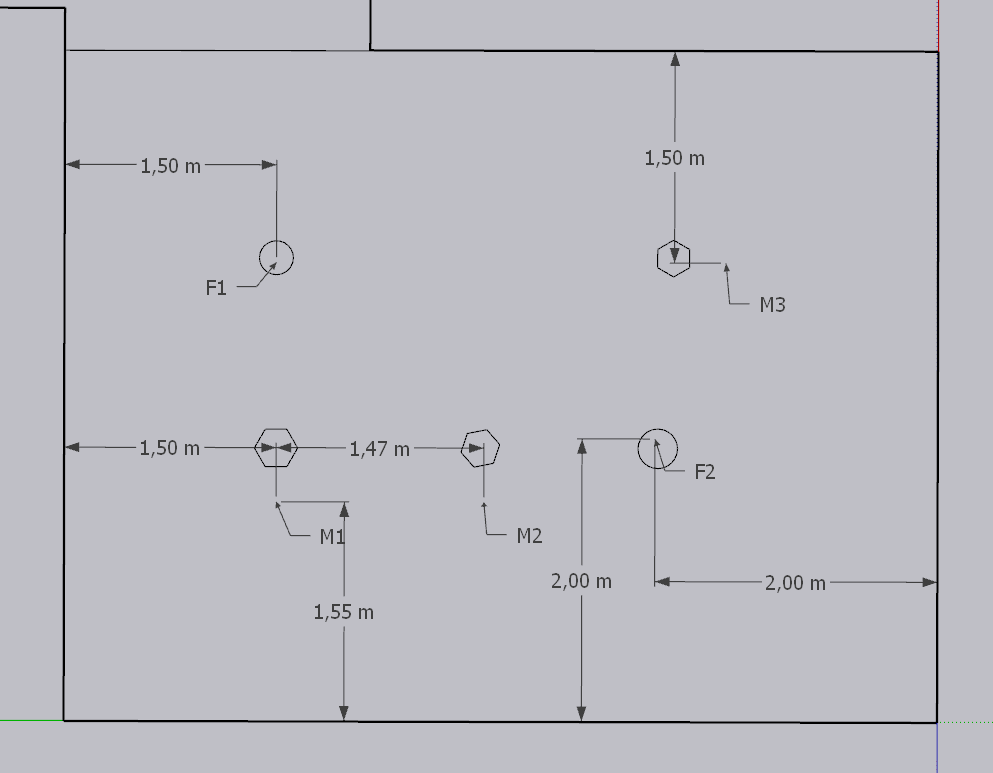
\includegraphics[width=6cm]{images/Posiciones RT/Posiciones Sala 1.png}
%     \caption{Posiciones de micrófono y fuente en Sala 1}
%     \label{fig:posiciones RT sala 1}
% \end{figure}
% \end{frame}
% \begin{frame}{Tiempo de reverberación}
%  ISO $3382$-$2$
%  \begin{figure}
%     \centering
%     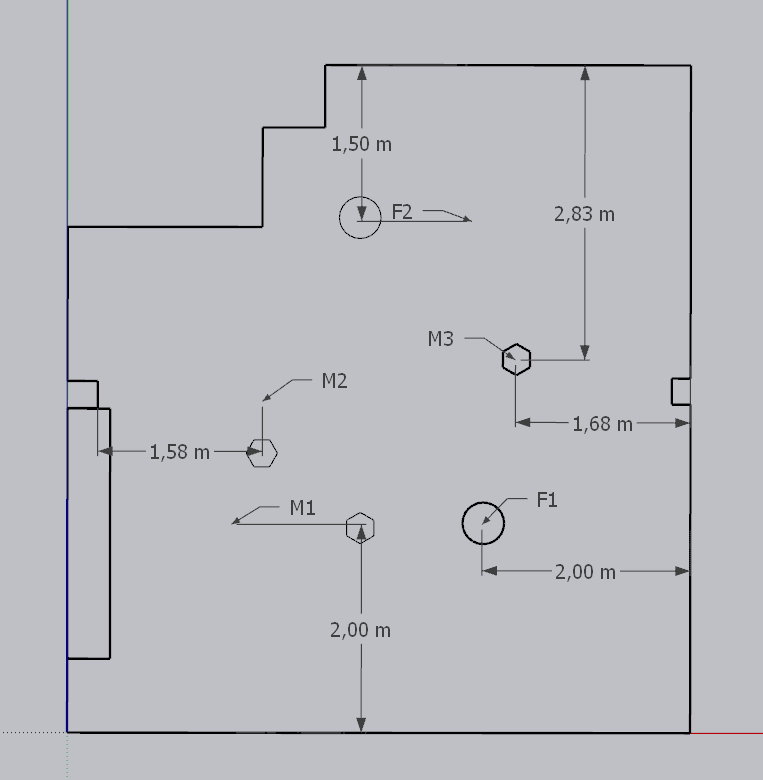
\includegraphics[width=5cm]{images/Posiciones RT/Posiciones Sala 2.png}
%     \caption{Posiciones de micrófono y fuente en Sala 2}
%     \label{fig:posiciones RT sala 2}
% \end{figure}
% \end{frame}
% \begin{frame}{Tiempo de reverberación}
%  ISO $3382$-$2$
%  \begin{figure}
%     \centering
%     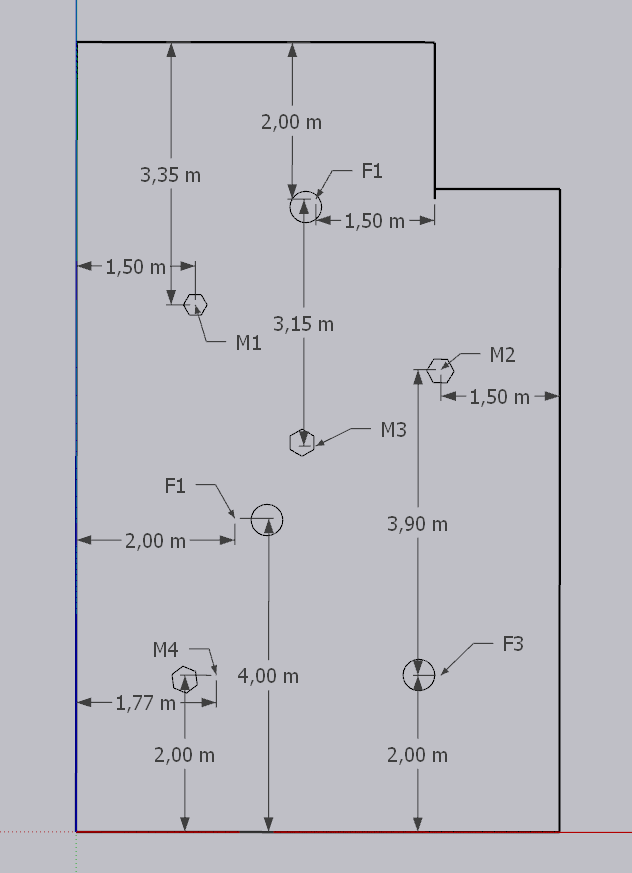
\includegraphics[width=4cm]{images/Posiciones RT/Posiciones Sala OCV.png}
%     \caption{Posiciones de micrófono y fuente en Sala de ensayo}
%     \label{fig:posiciones RT sala de ensayo}
% \end{figure}
% \end{frame}

\section{Recomendaciones}
\begin{frame}{Salas de reuniones}
    \begin{table}[H]
    \centering
    \caption{Parámetros objetivos para salas de reuniones}
    \label{tab: parametros objetivos sala de reuniones}
    \begin{tabular}{|c|l|c|c|}
    \hline
    \textbf{Parámetro} & \textbf{Uso }                 & \textbf{Valores}     & \textbf{Fuente}  \\ \hline
    Curvas NC & Para salas de juntas & $25$ - $30$ & Recuero \\ \hline
    $T_{target}$ & Speech/Lecture (A2) & 0.6 & DIN18041 \\ \hline
    $C_{50speech}$  & Para la voz &  $C_{50}>0$         &  Marshall  \\ \hline  
    STI & Transmisión del habla & STI $>$ 0.45 & ISO 9921\\ \hline
    \end{tabular}
    
\end{table}
\end{frame}
\begin{frame}{Sala de ensayo}
    \begin{table}[H]
    \centering
    \caption{Parámetros objetivos para sala de ensayo}
    \label{tab: parametros objetivos sala de ensayo}
    \begin{tabular}{|c|l|c|c|}
    \hline
    \textbf{Parámetro} & \textbf{Uso}                  & \textbf{Valores}     & \textbf{Fuente}  \\ \hline
    Curvas NC & Salas de conciertos y teatros de ópera & $20$ - $25$ & Recuero \\ \hline
    $RT_{mid}$ & Sala de conciertos (música de cámara) & 1.3 - 1.7 & Carrión \\ \hline
    $C_{80}$  & Para música sinfónica &  $-2<C_{80}<2$         &  Marshall  \\ \hline   
    $D_{50}$  & Salas de concierto         &  $D_{50}<$ 0.5         &  Thiele \\ \hline
    \end{tabular}
    
\end{table}
\end{frame}

\section{Parámetros acústicos obtenidos}

\begin{frame}{Ruido de fondo}
\begin{figure}
    \centering
    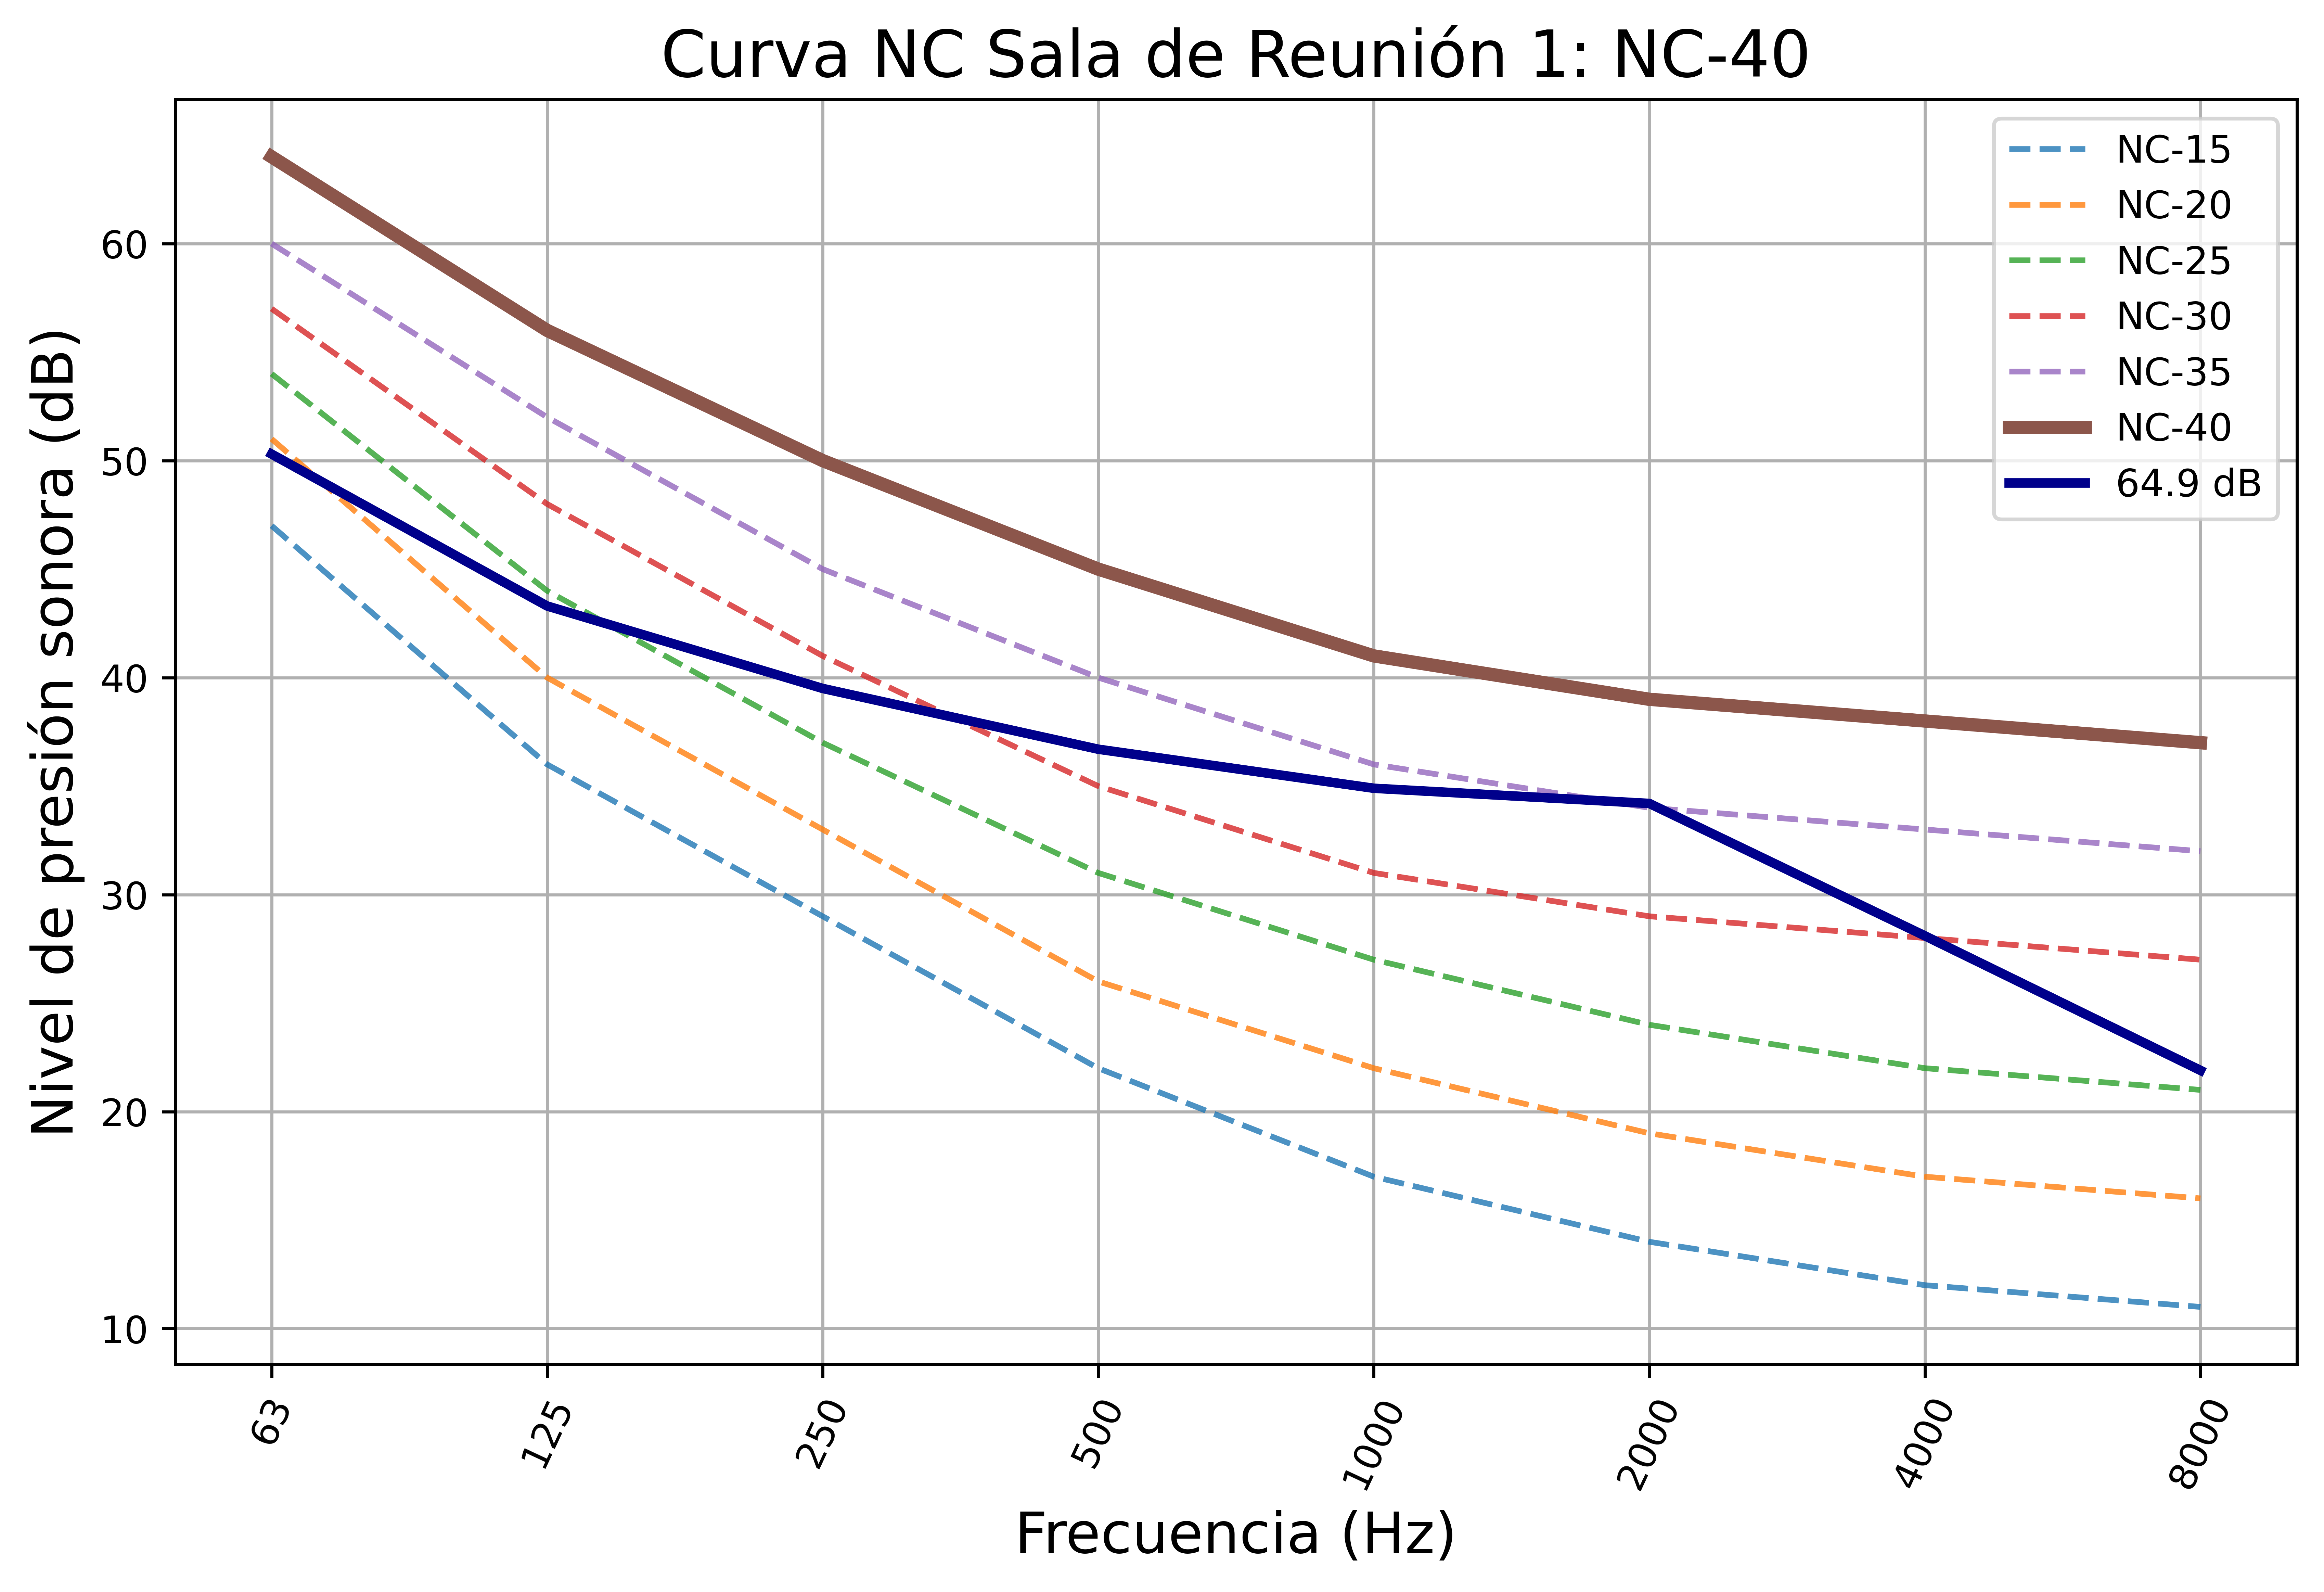
\includegraphics[width=9cm]{images/Curvas NC/NC reunion 1.png}
    \caption{Curva NC Sala de reunión 1}
    \label{fig:nc-sala1}
\end{figure}
\end{frame}

\begin{frame}{Ruido de fondo}
\begin{figure}
    \centering
    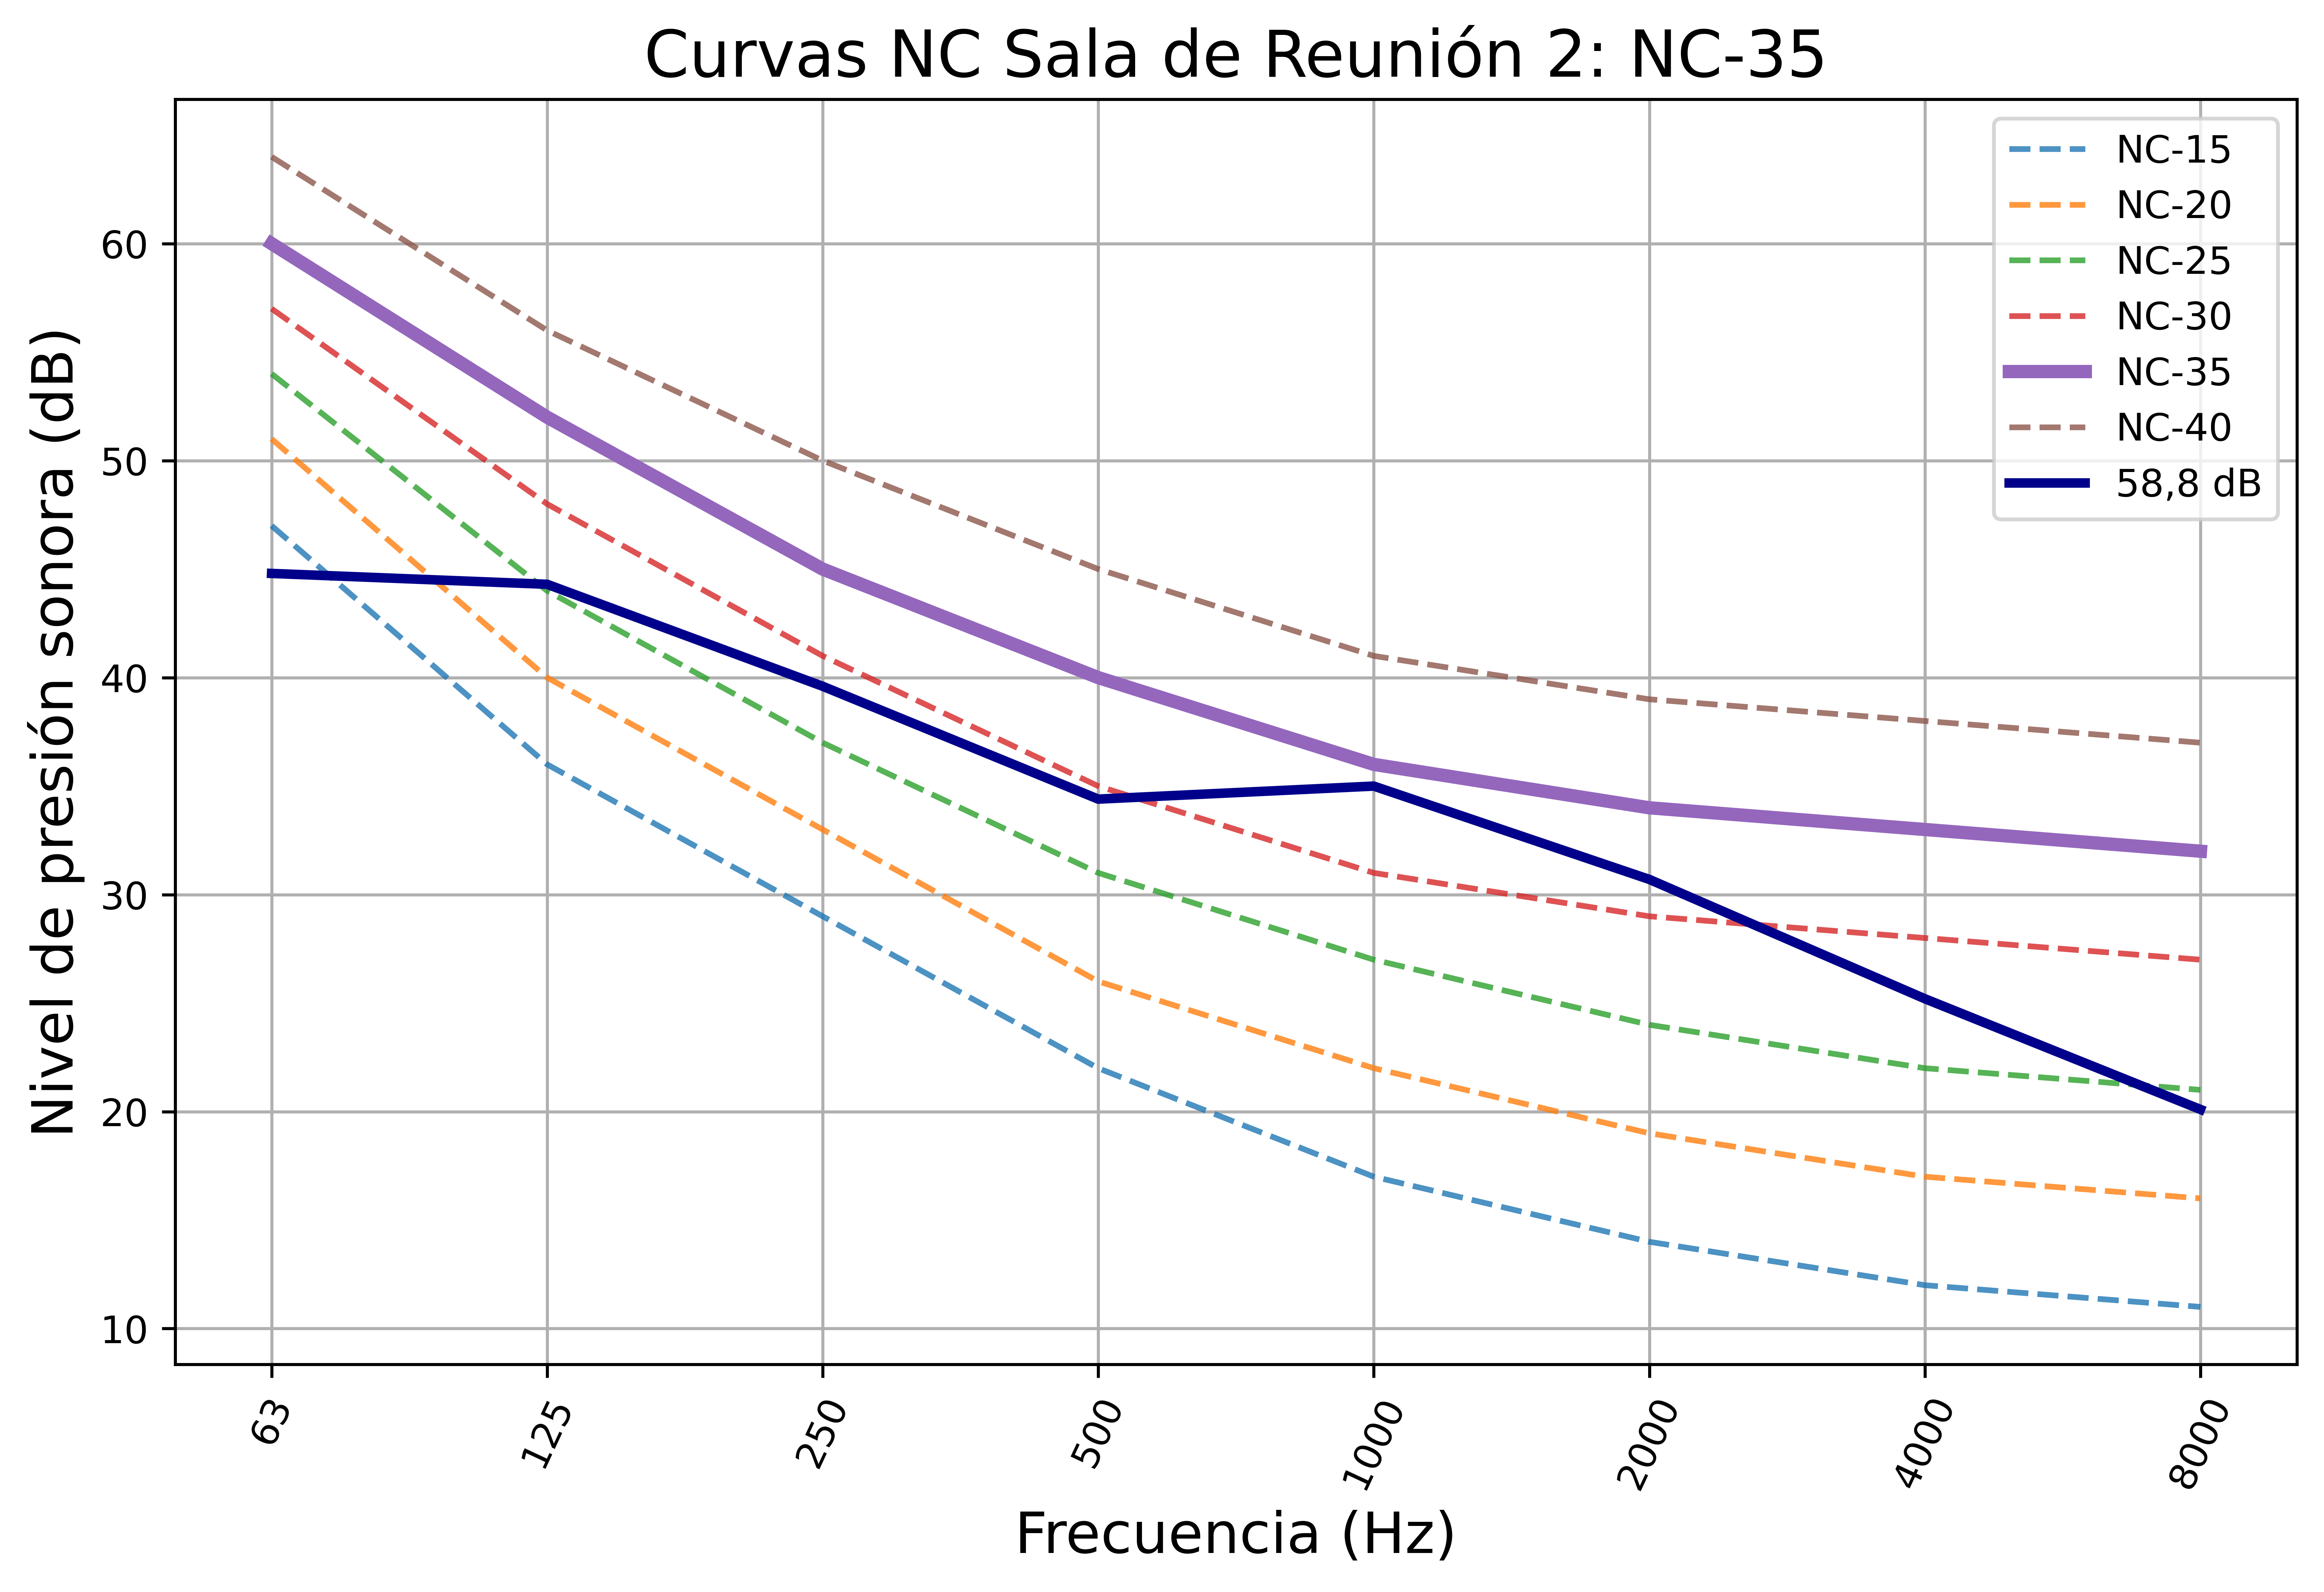
\includegraphics[width=9cm]{images/Curvas NC/NC reunion 2.png}
    \caption{Curva NC Sala de reunión 2}
    \label{fig:nc-sala2}
\end{figure}
    
\end{frame}

\begin{frame}{Ruido de fondo}
\begin{figure}
    \centering
    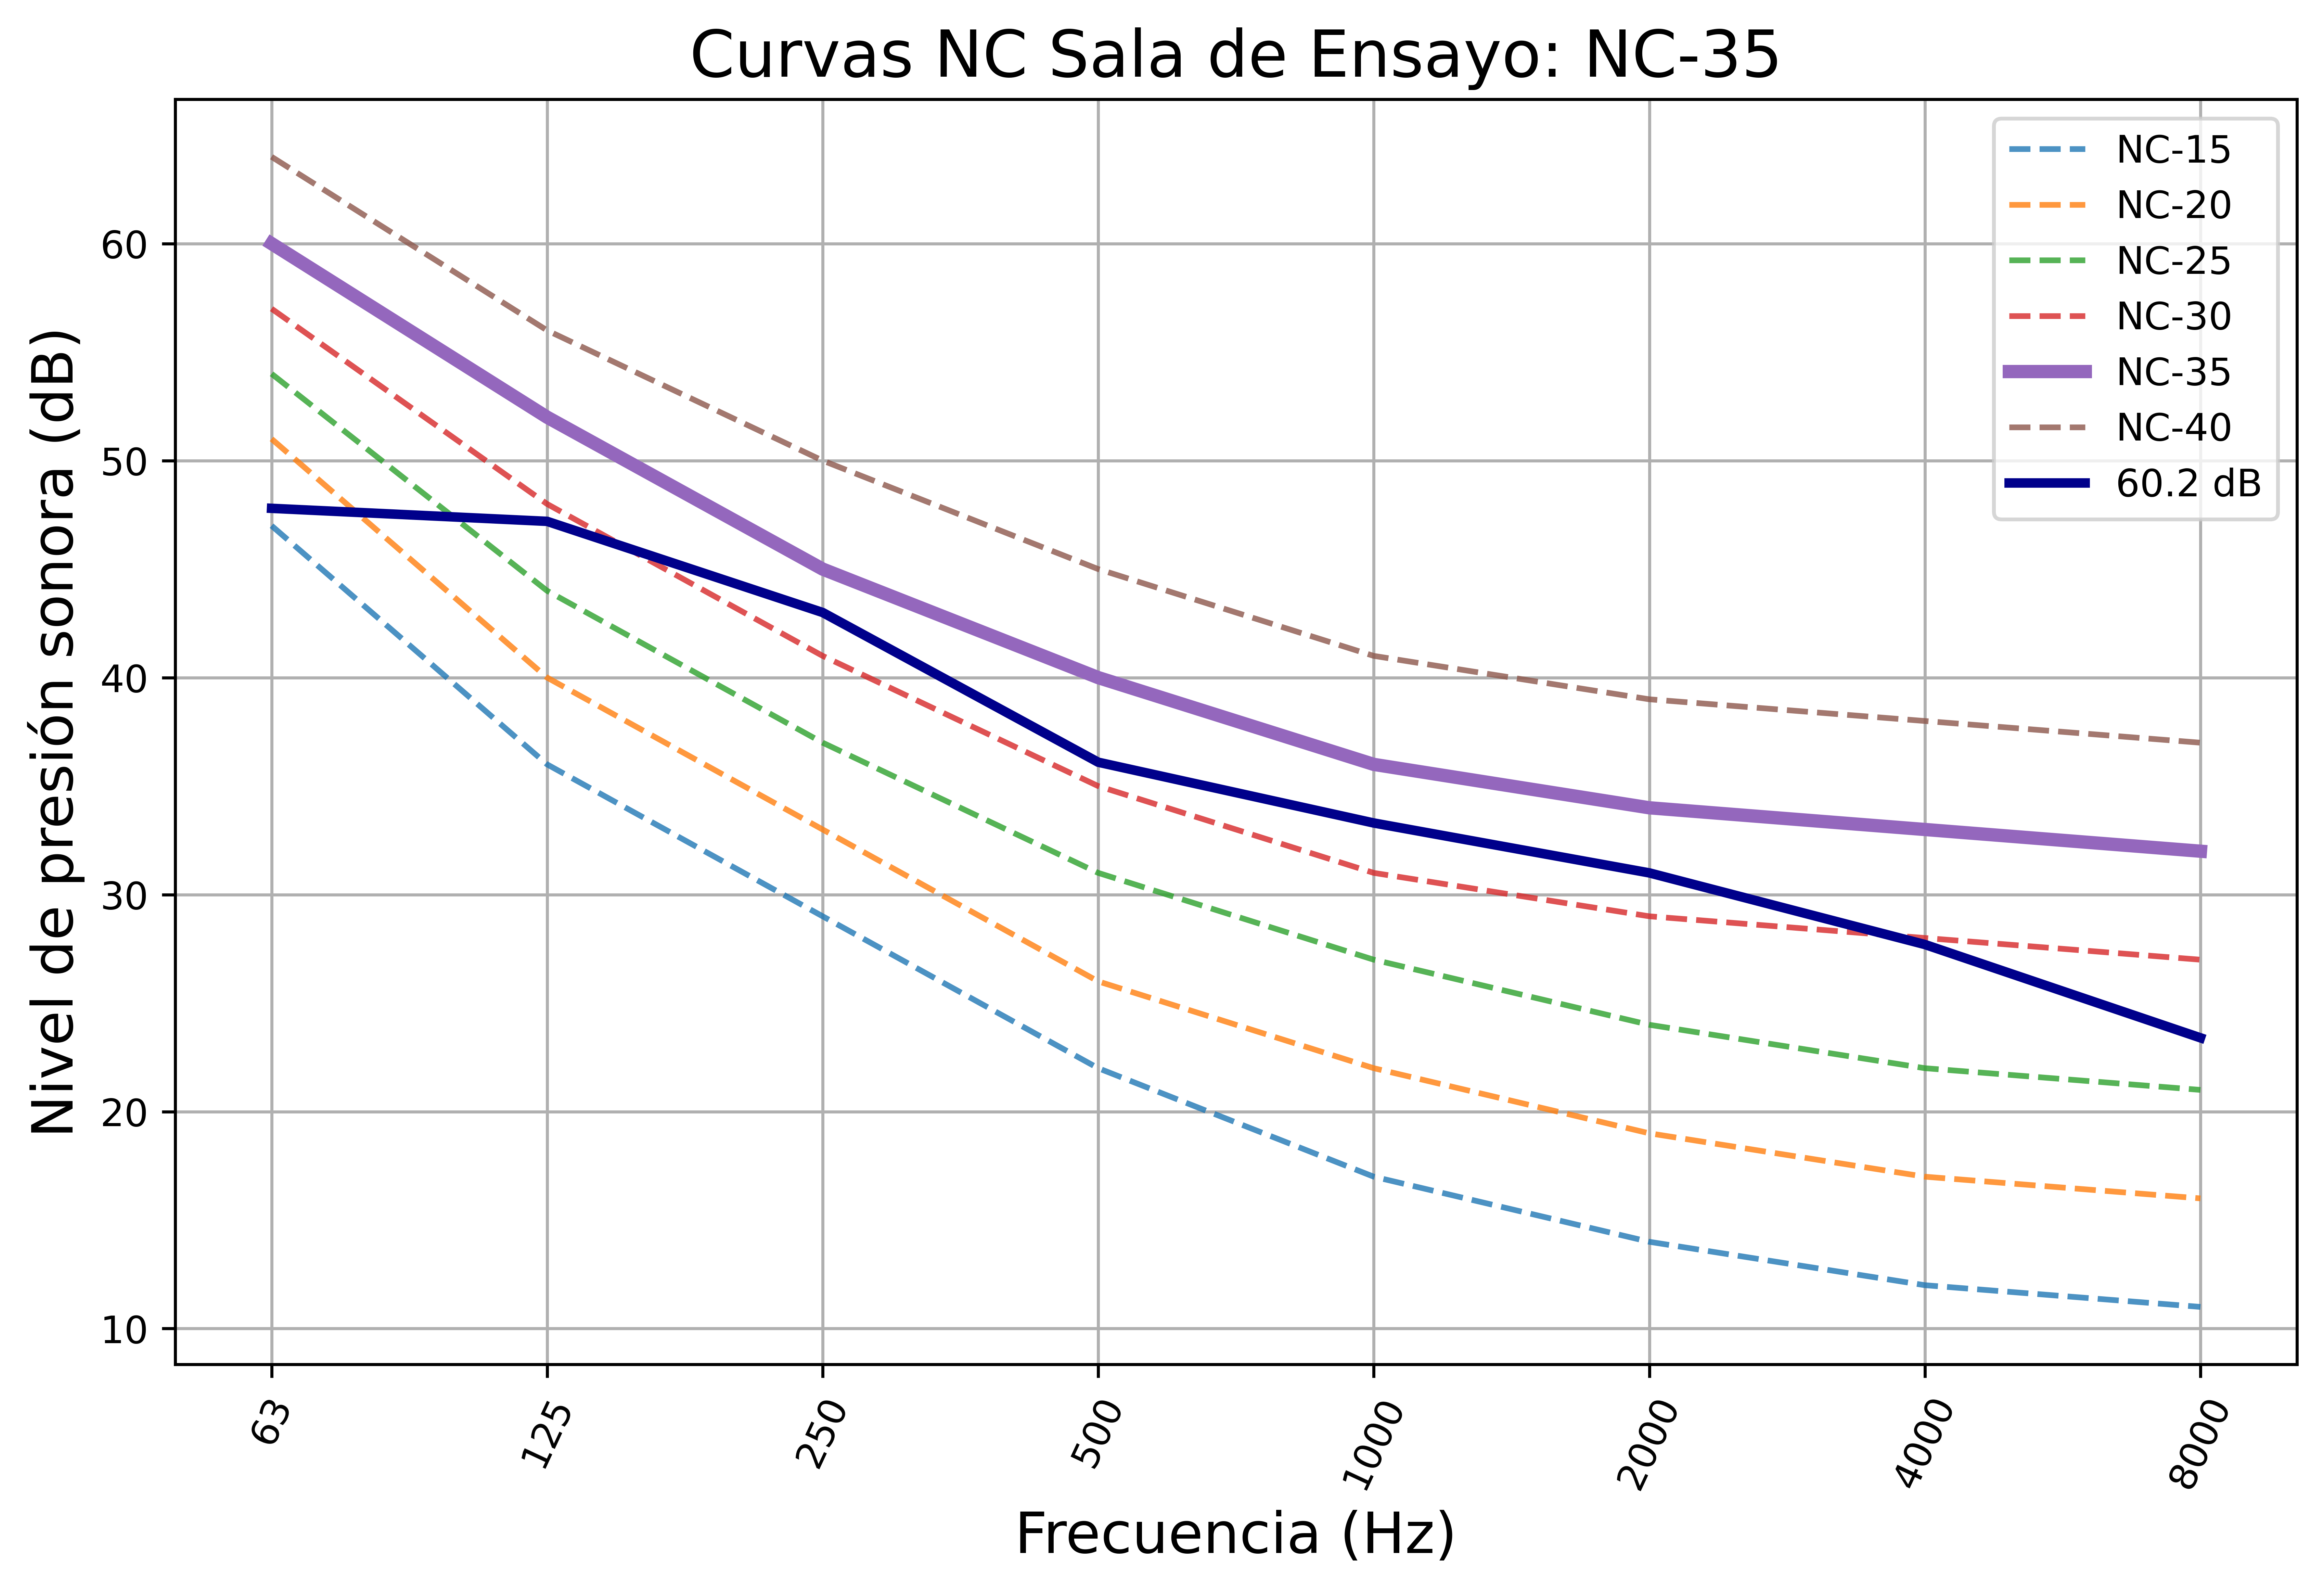
\includegraphics[width=9cm]{images/Curvas NC/NC ensayo.png}
    \caption{Curva NC Sala de ensayo}
    \label{fig:nc-ensayo}
\end{figure}
\end{frame}

% \begin{frame}{Ruido de fondo}
% \begin{figure}
%     \centering
%     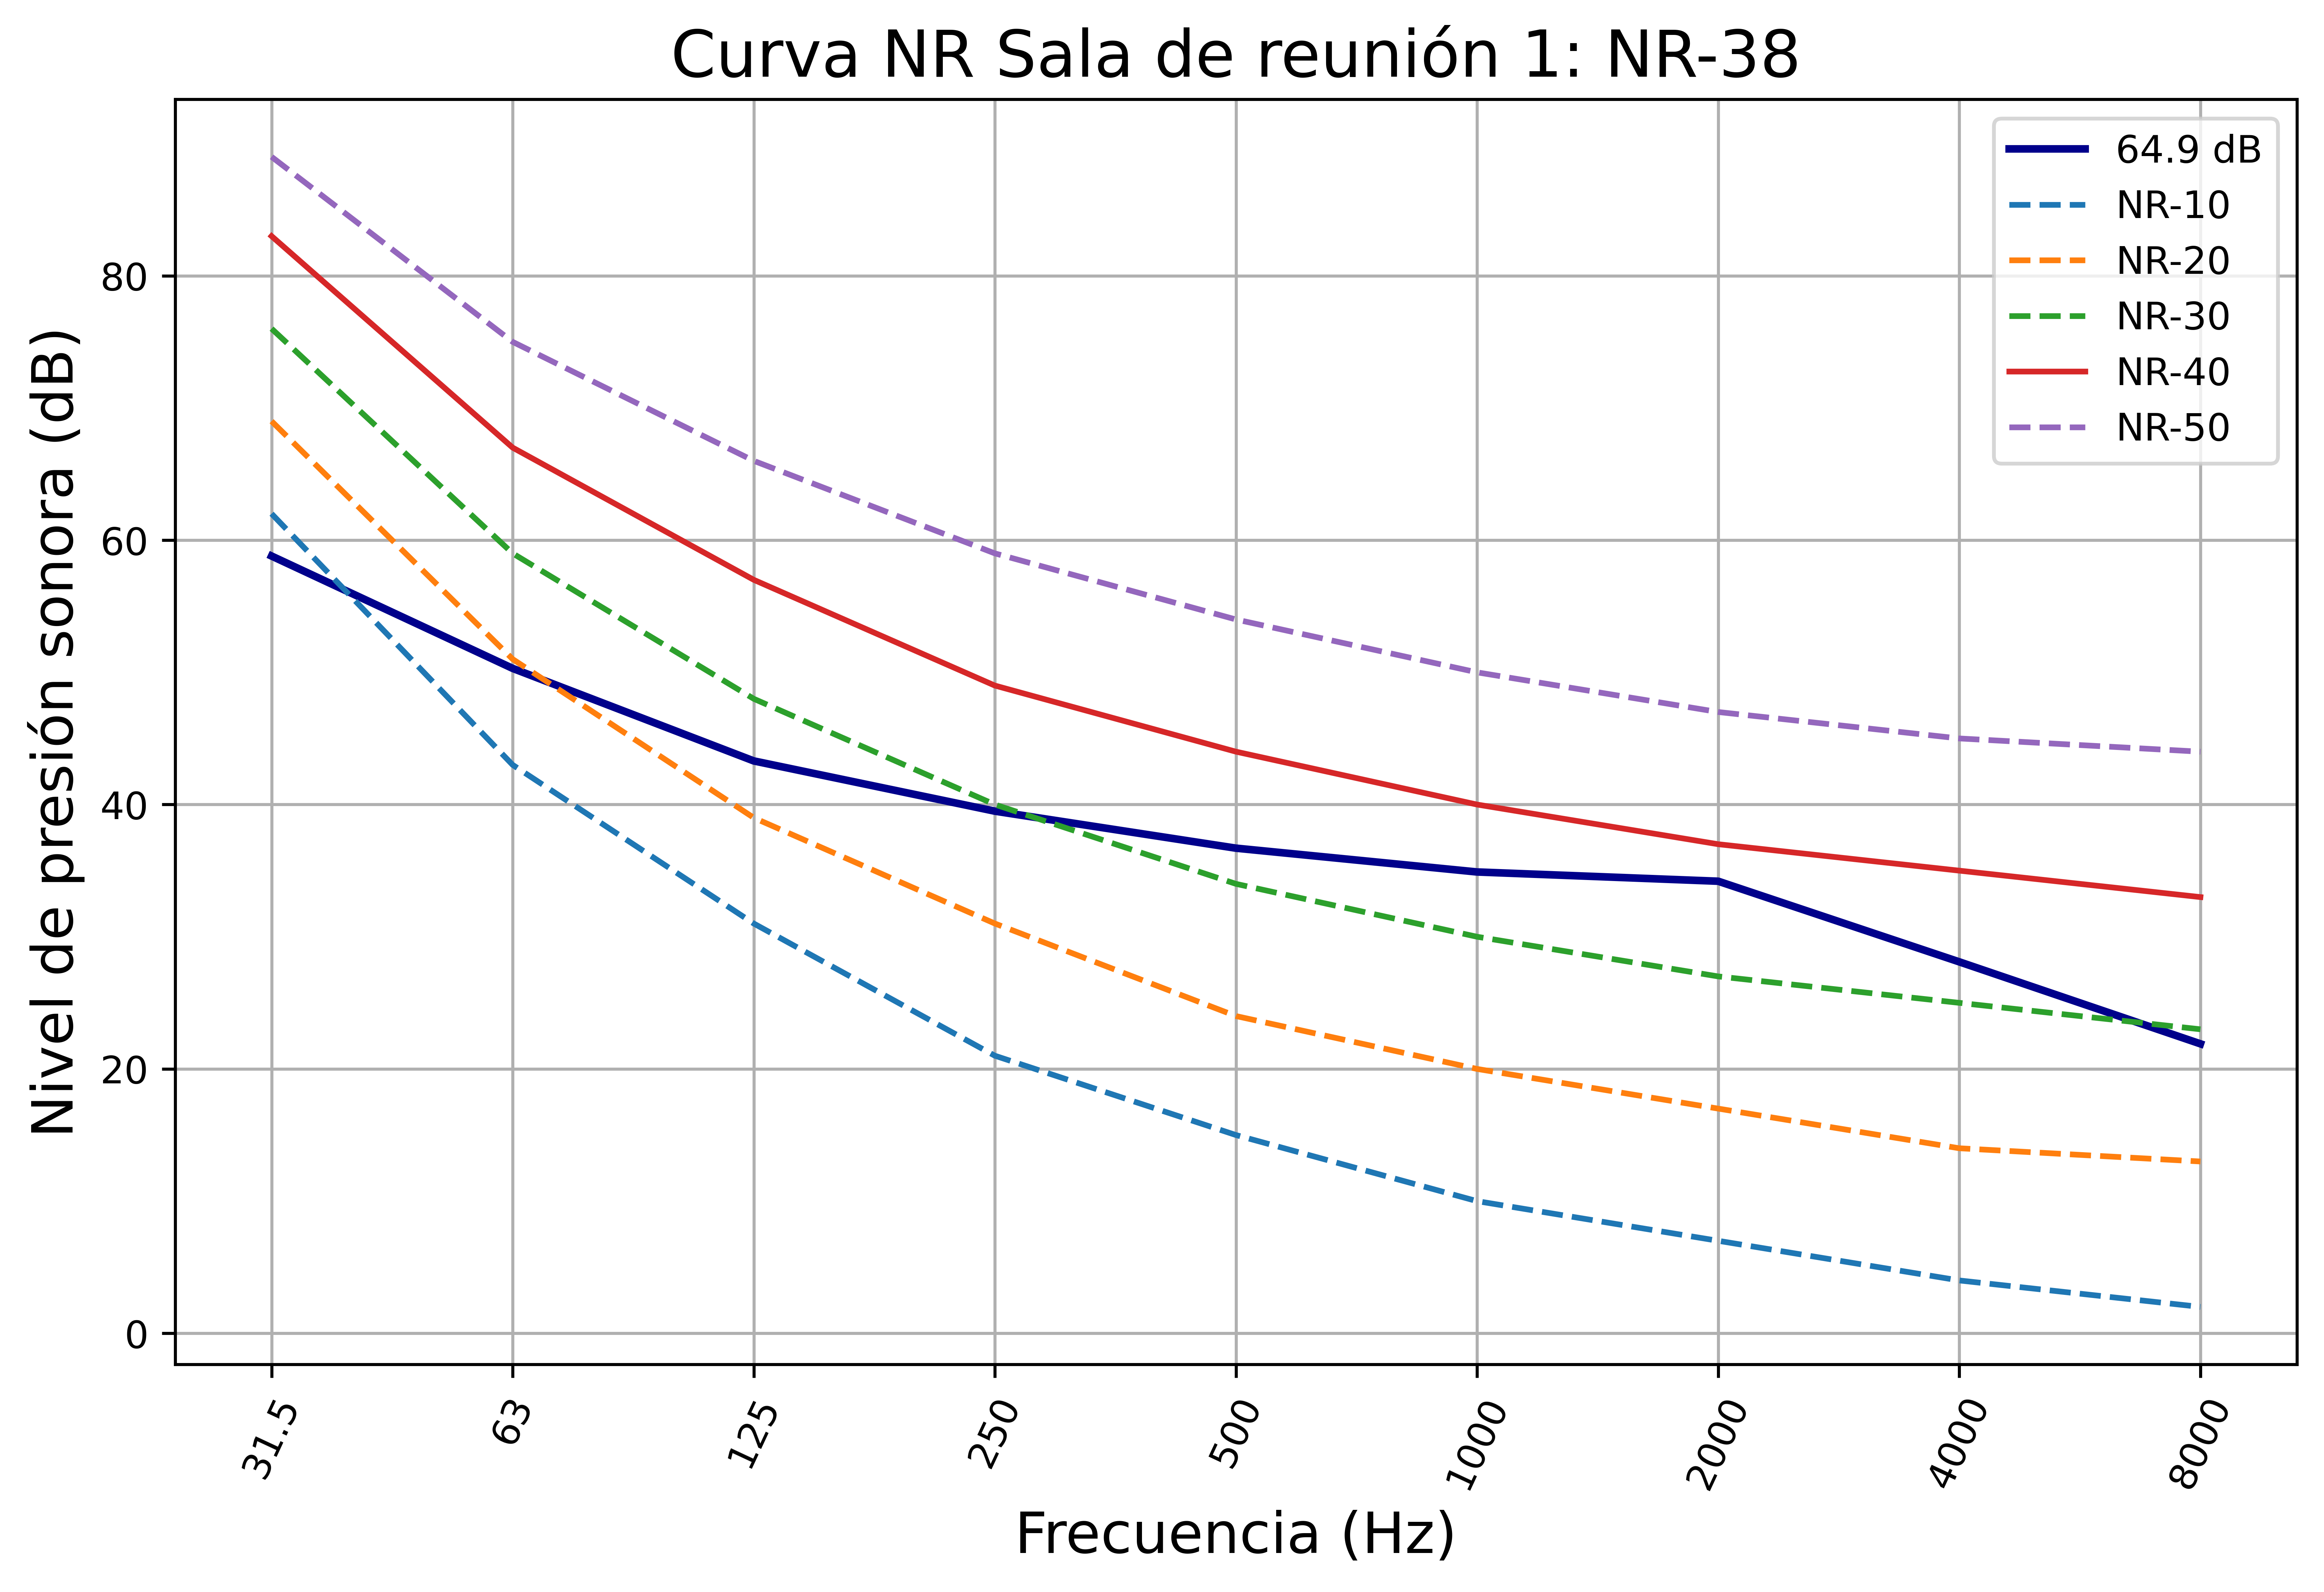
\includegraphics[width=9cm]{images/Curvas NR/NR reunion 1.png}
%     \caption{Curva NR Sala de reunión 1}
%     \label{fig:nr-sala1}
% \end{figure}
% \end{frame}

% \begin{frame}{Ruido de fondo}
% \begin{figure}
%     \centering
%     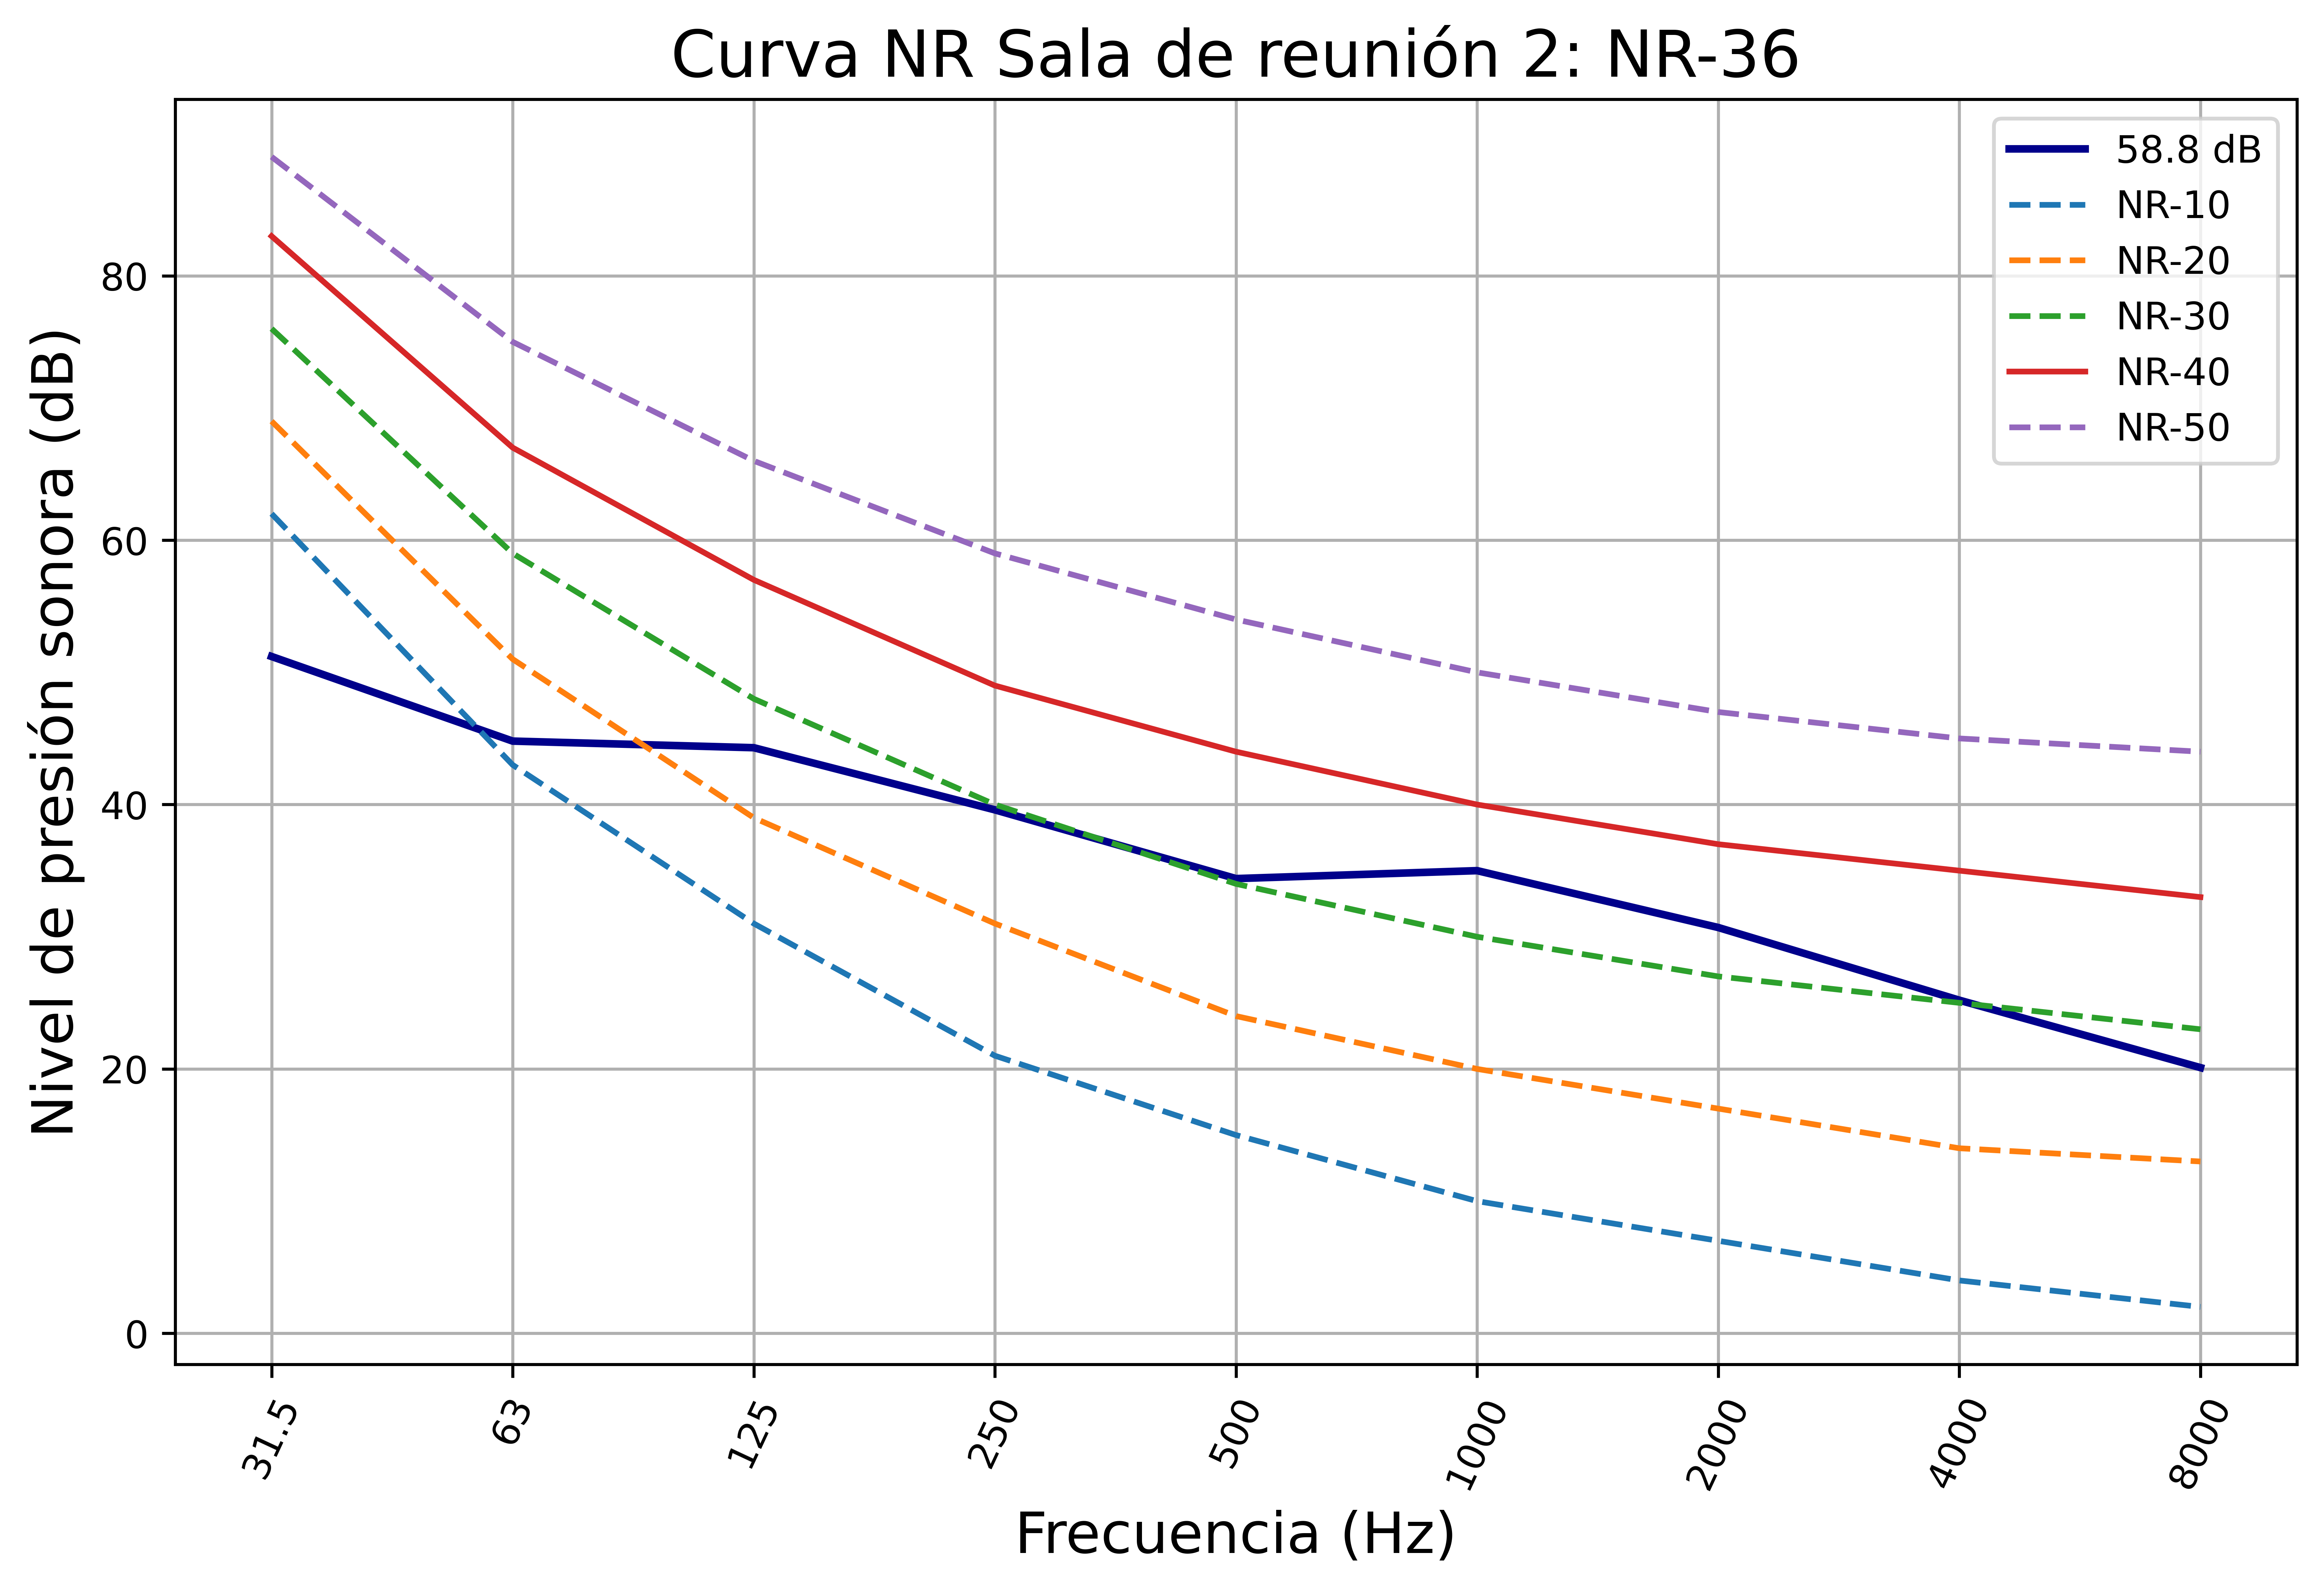
\includegraphics[width=9cm]{images/Curvas NR/NR reunion 2.png}
%     \caption{Curva NR Sala de reunión 2}
%     \label{fig:nr-sala2}
% \end{figure}
    
% \end{frame}

% \begin{frame}{Ruido de fondo}
% \begin{figure}
%     \centering
%     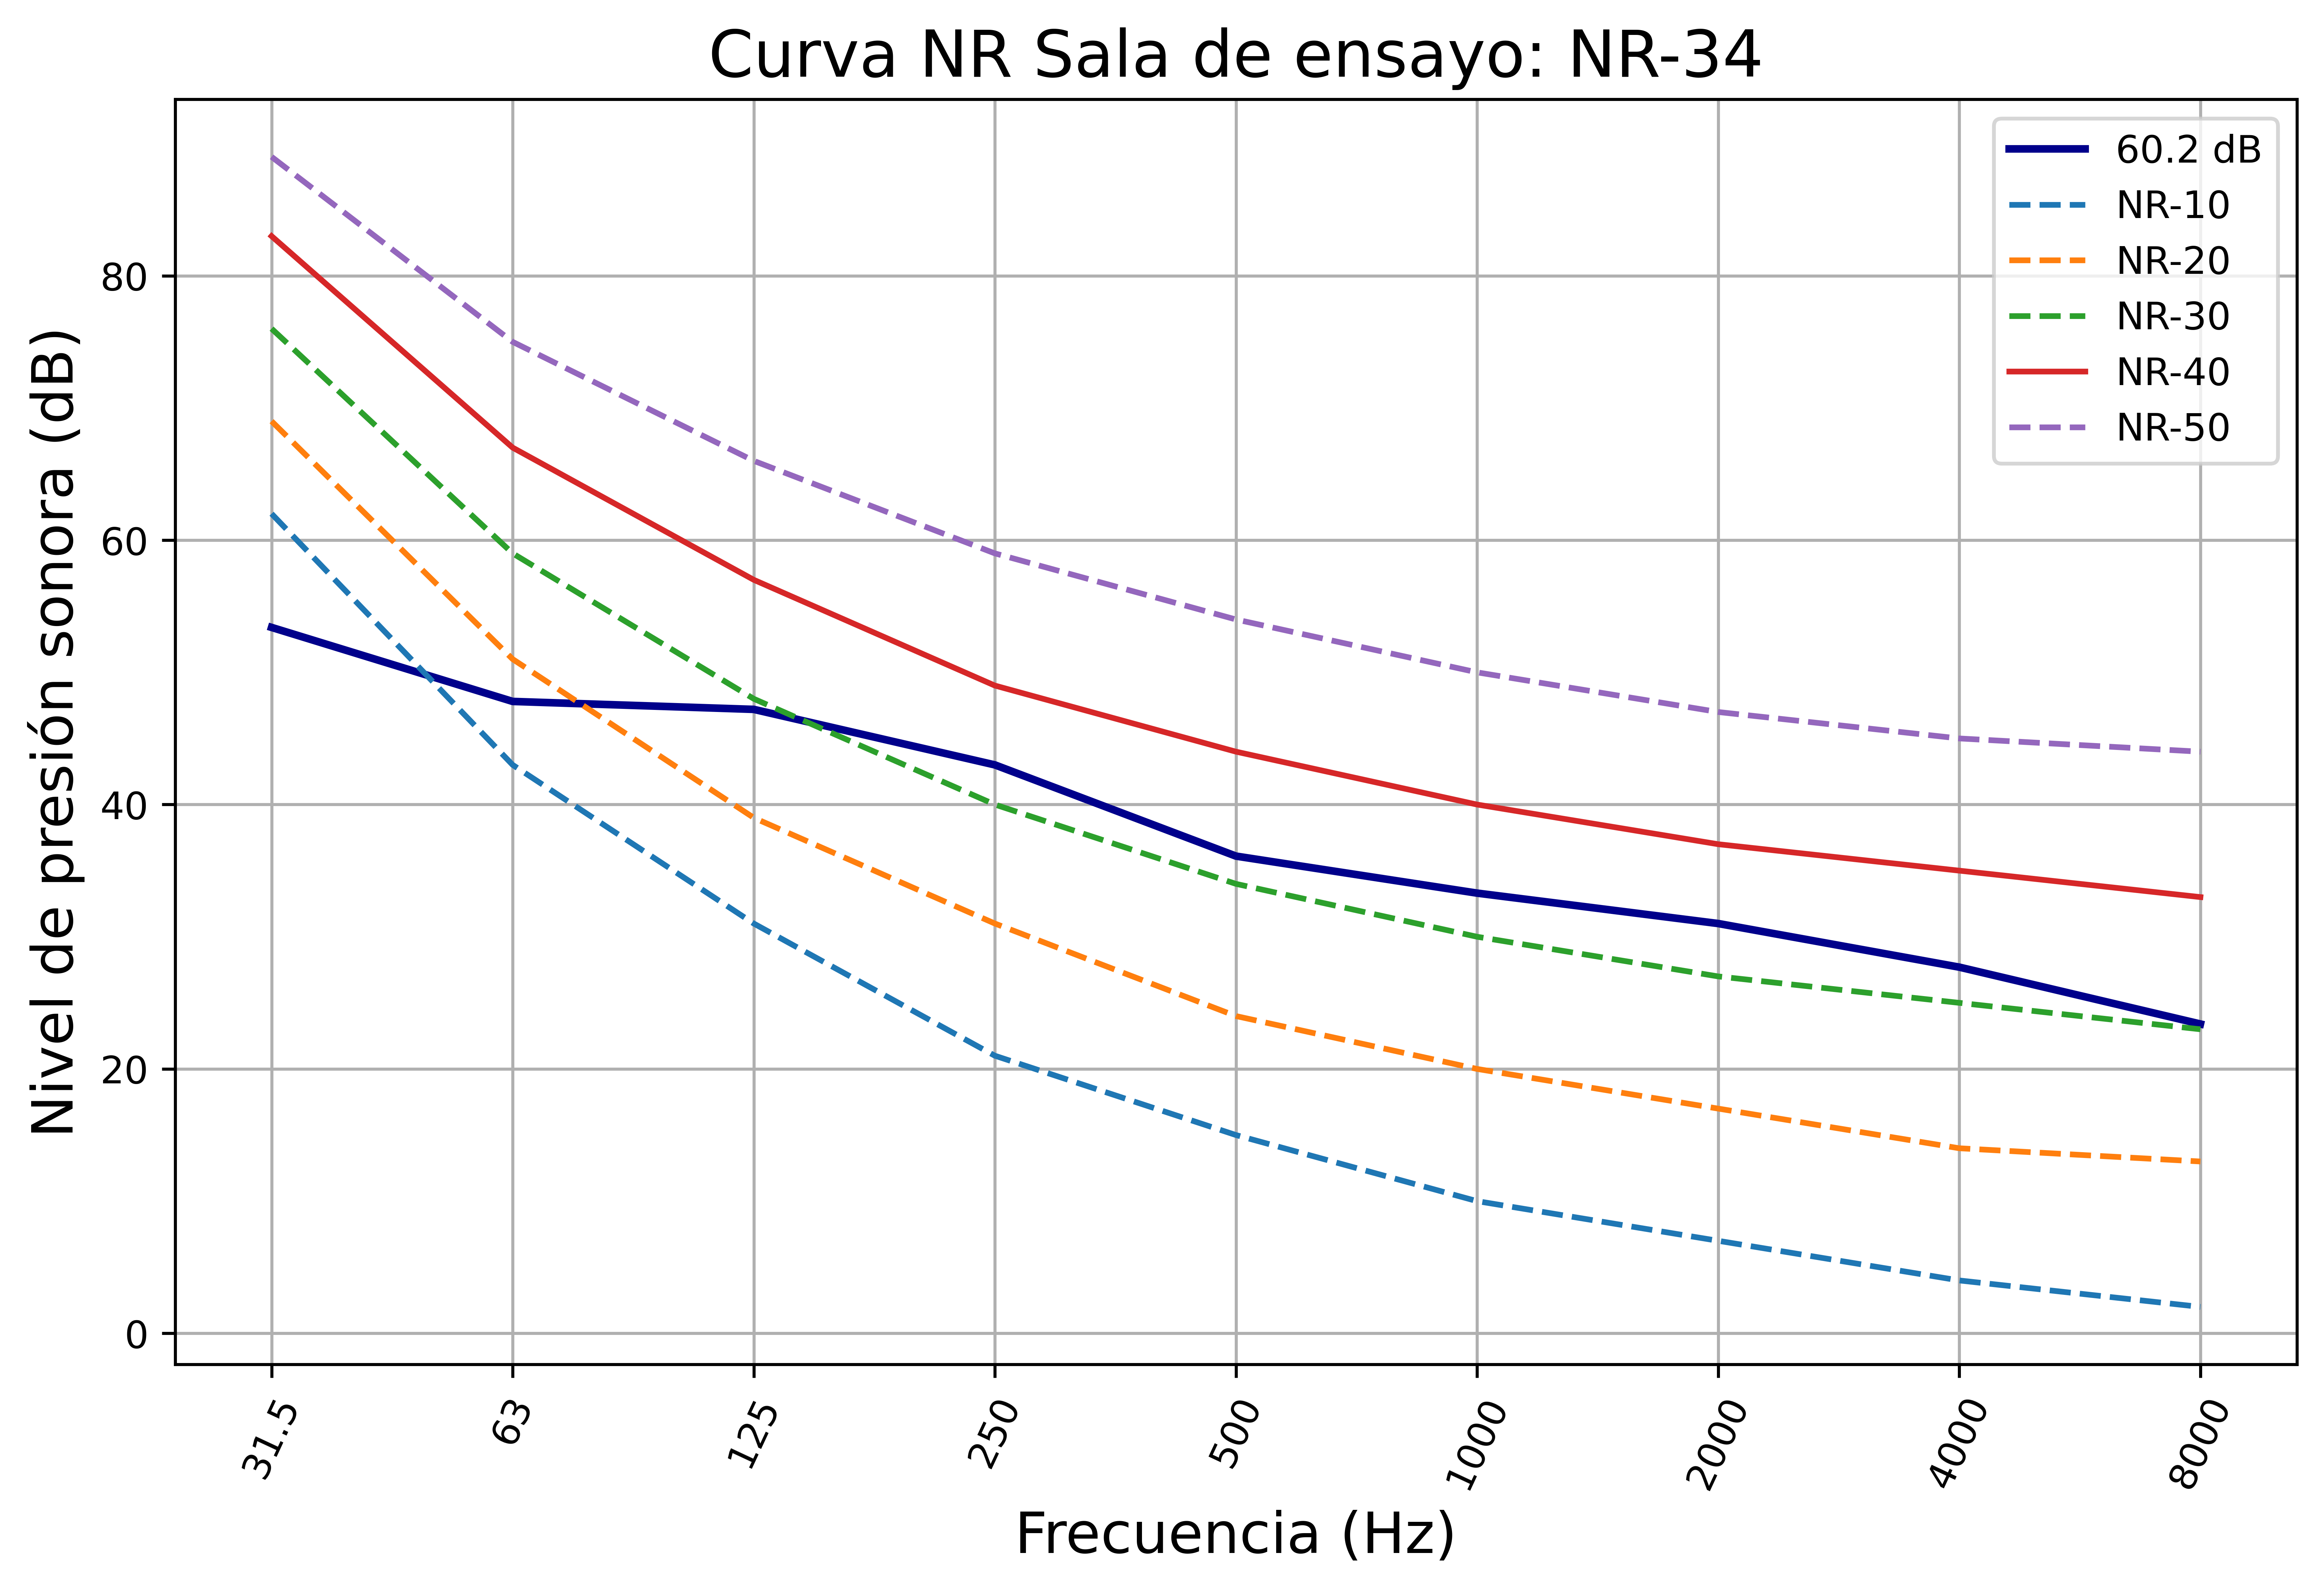
\includegraphics[width=9cm]{images/Curvas NR/NR ensayo.png}
%     \caption{Curva NR Sala de ensayo}
%     \label{fig:nr-ensayo}
% \end{figure}
% \end{frame}
\begin{frame}{Ruido de fondo}
    A continuación, se muestra una tabla donde se observa el estado de cada sala con respecto a lo recomendado.
    \begin{table}[H]
    \centering
    \caption{Estado de parámetros de ruido de fondo por sala}
    \label{tab: cumplimiento de Rdf}
    \begin{tabular}{|l|c|c|c|}
    \hline
    \textbf{Salones} & \textbf{\begin{tabular}[c]{@{}c@{}}Curva NC\\  recomendada\end{tabular}} & \textbf{\begin{tabular}[c]{@{}c@{}}Curva NC\\  medida\end{tabular}} & \textbf{Estado} \\ \hline
    Sala de reunión 1 & $25$ - $30$ & $40$ & \textcolor{red}{No cumple}\\ \hline
    Sala de reunión 2 & $25$ - $30$ & $35$ & \textcolor{red}{No cumple}\\ \hline
    Sala de ensayo & $20$ - $25$ & $35$ & \textcolor{red}{No cumple} \\ \hline
    \end{tabular}
    
    \end{table}
\end{frame}


% \begin{frame}{Tiempo de reverberación}
%     \begin{figure}
%         \centering
%         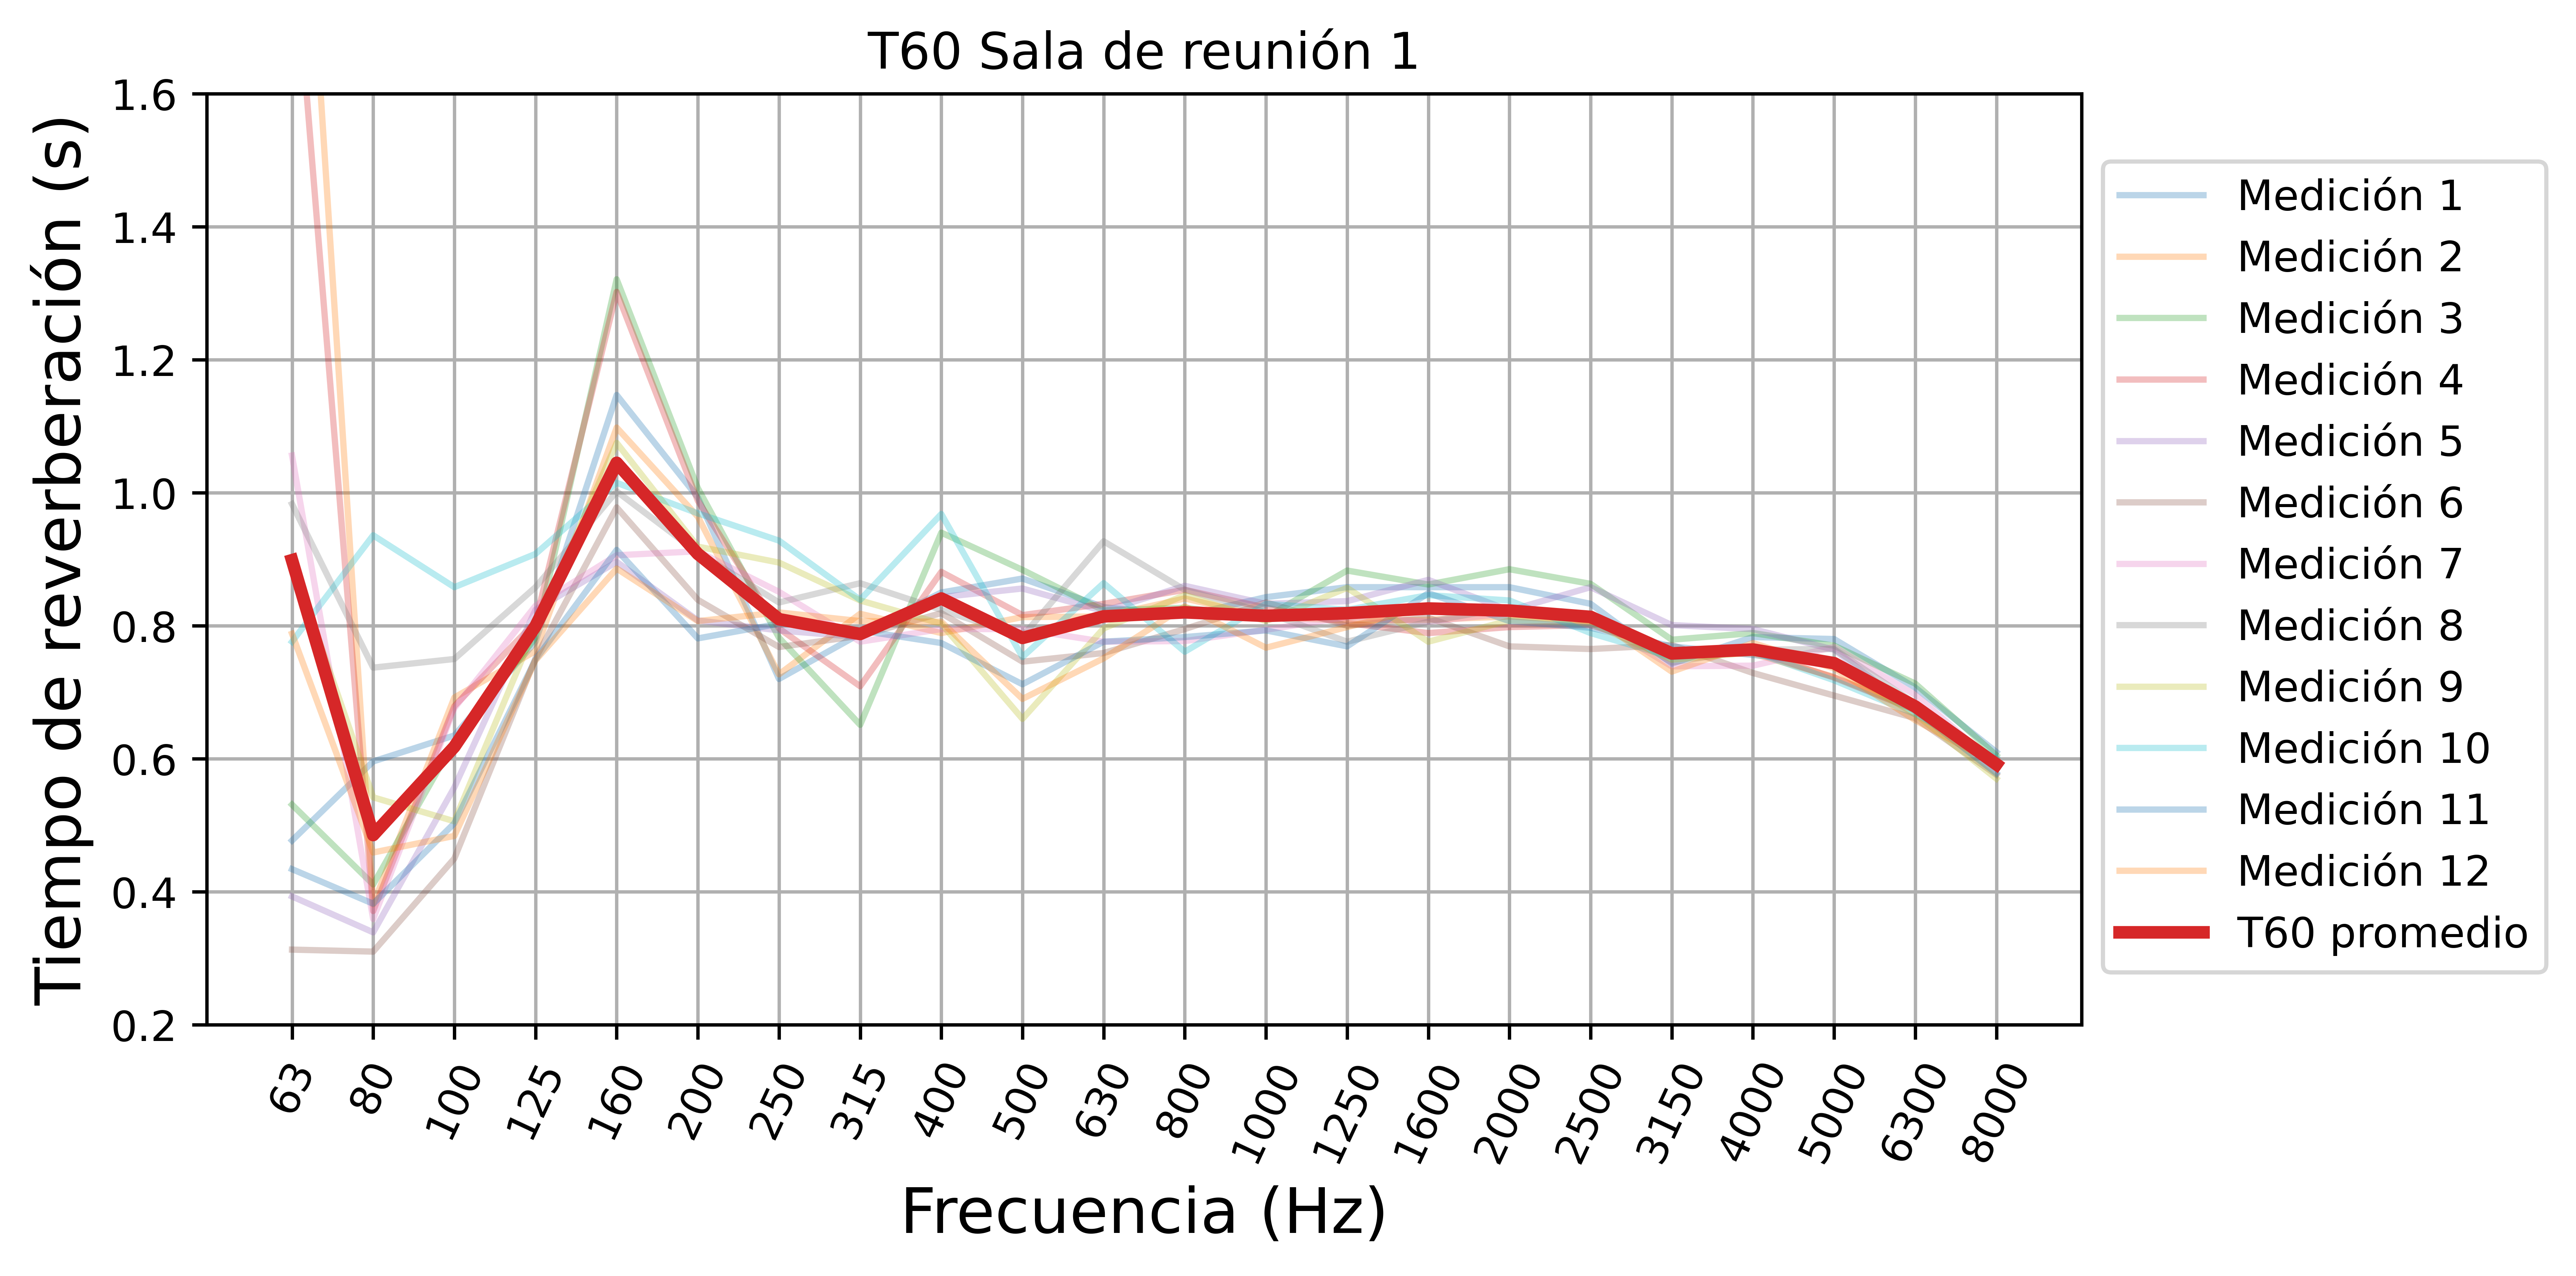
\includegraphics[width=10cm]{images/Tiempo de reverberación/T60_Sala_reunion_1.png}
%         \caption{Tiempo de reverberación en sala de reunión 1}
%         \label{fig:RT sala 1}
%     \end{figure}
% \end{frame}

% \begin{frame}{Tiempo de reverberación}
%     \begin{figure}
%         \centering
%         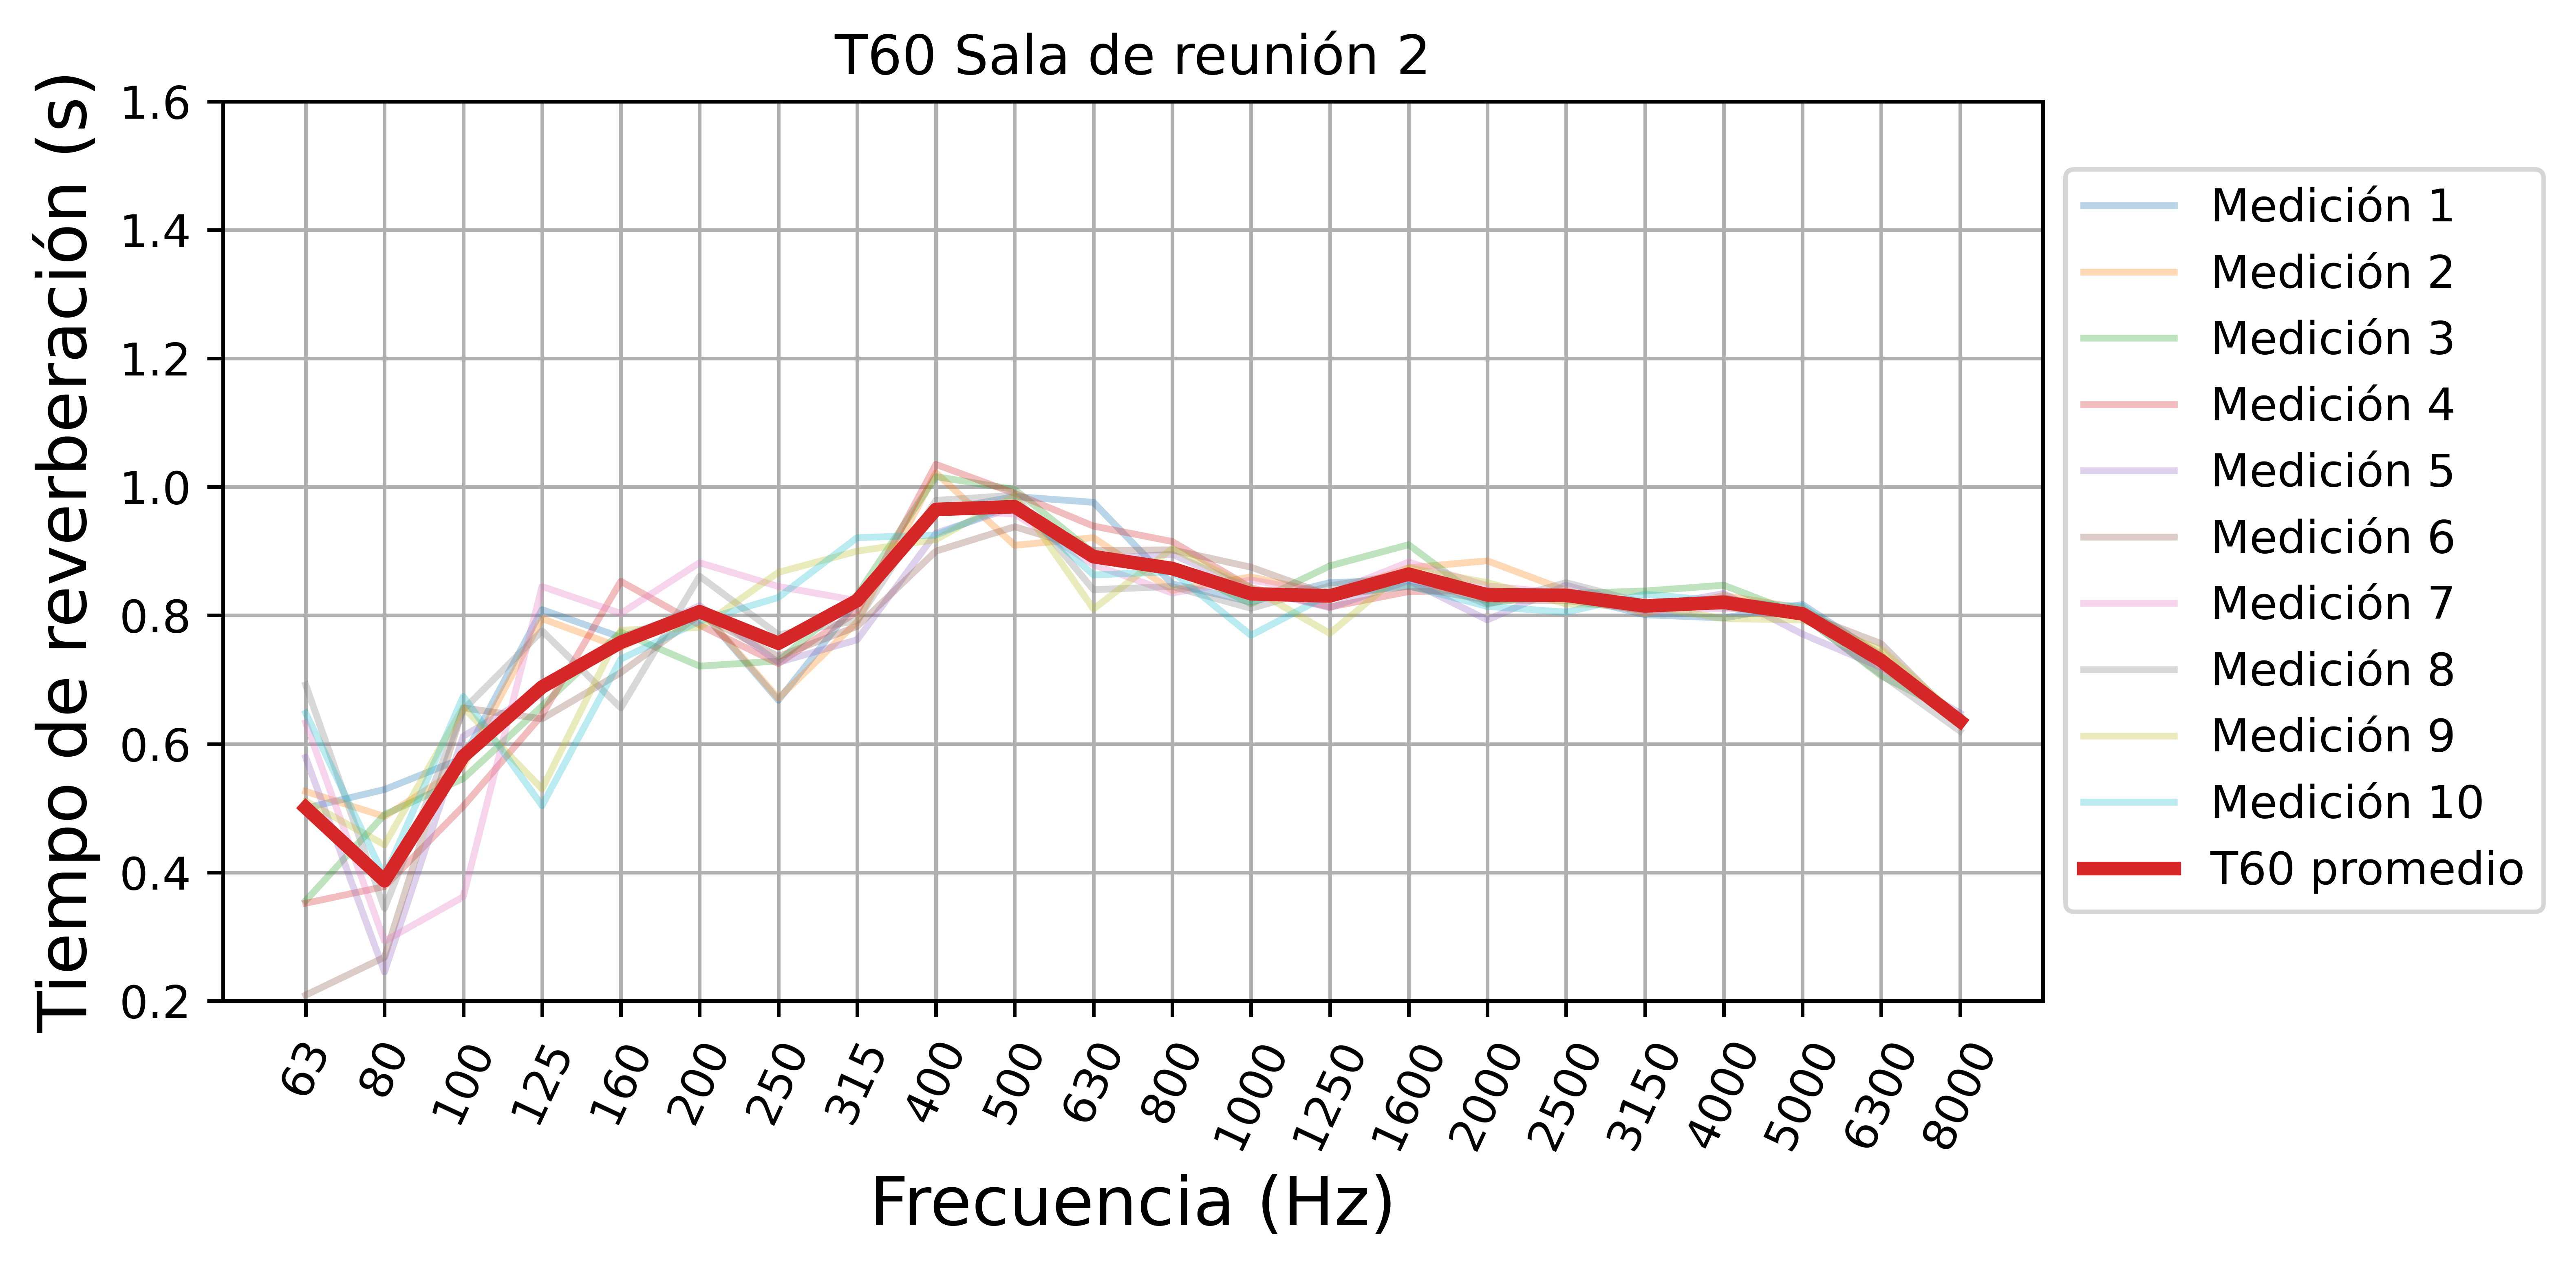
\includegraphics[width=10cm]{images/Tiempo de reverberación/T60_Sala_reunion_2.png}
%         \caption{Tiempo de reverberación en sala de reunión 2}
%         \label{fig:RT sala 2}
%     \end{figure}
% \end{frame}

% \begin{frame}{Tiempo de reverberación}
%     \begin{figure}
%         \centering
%         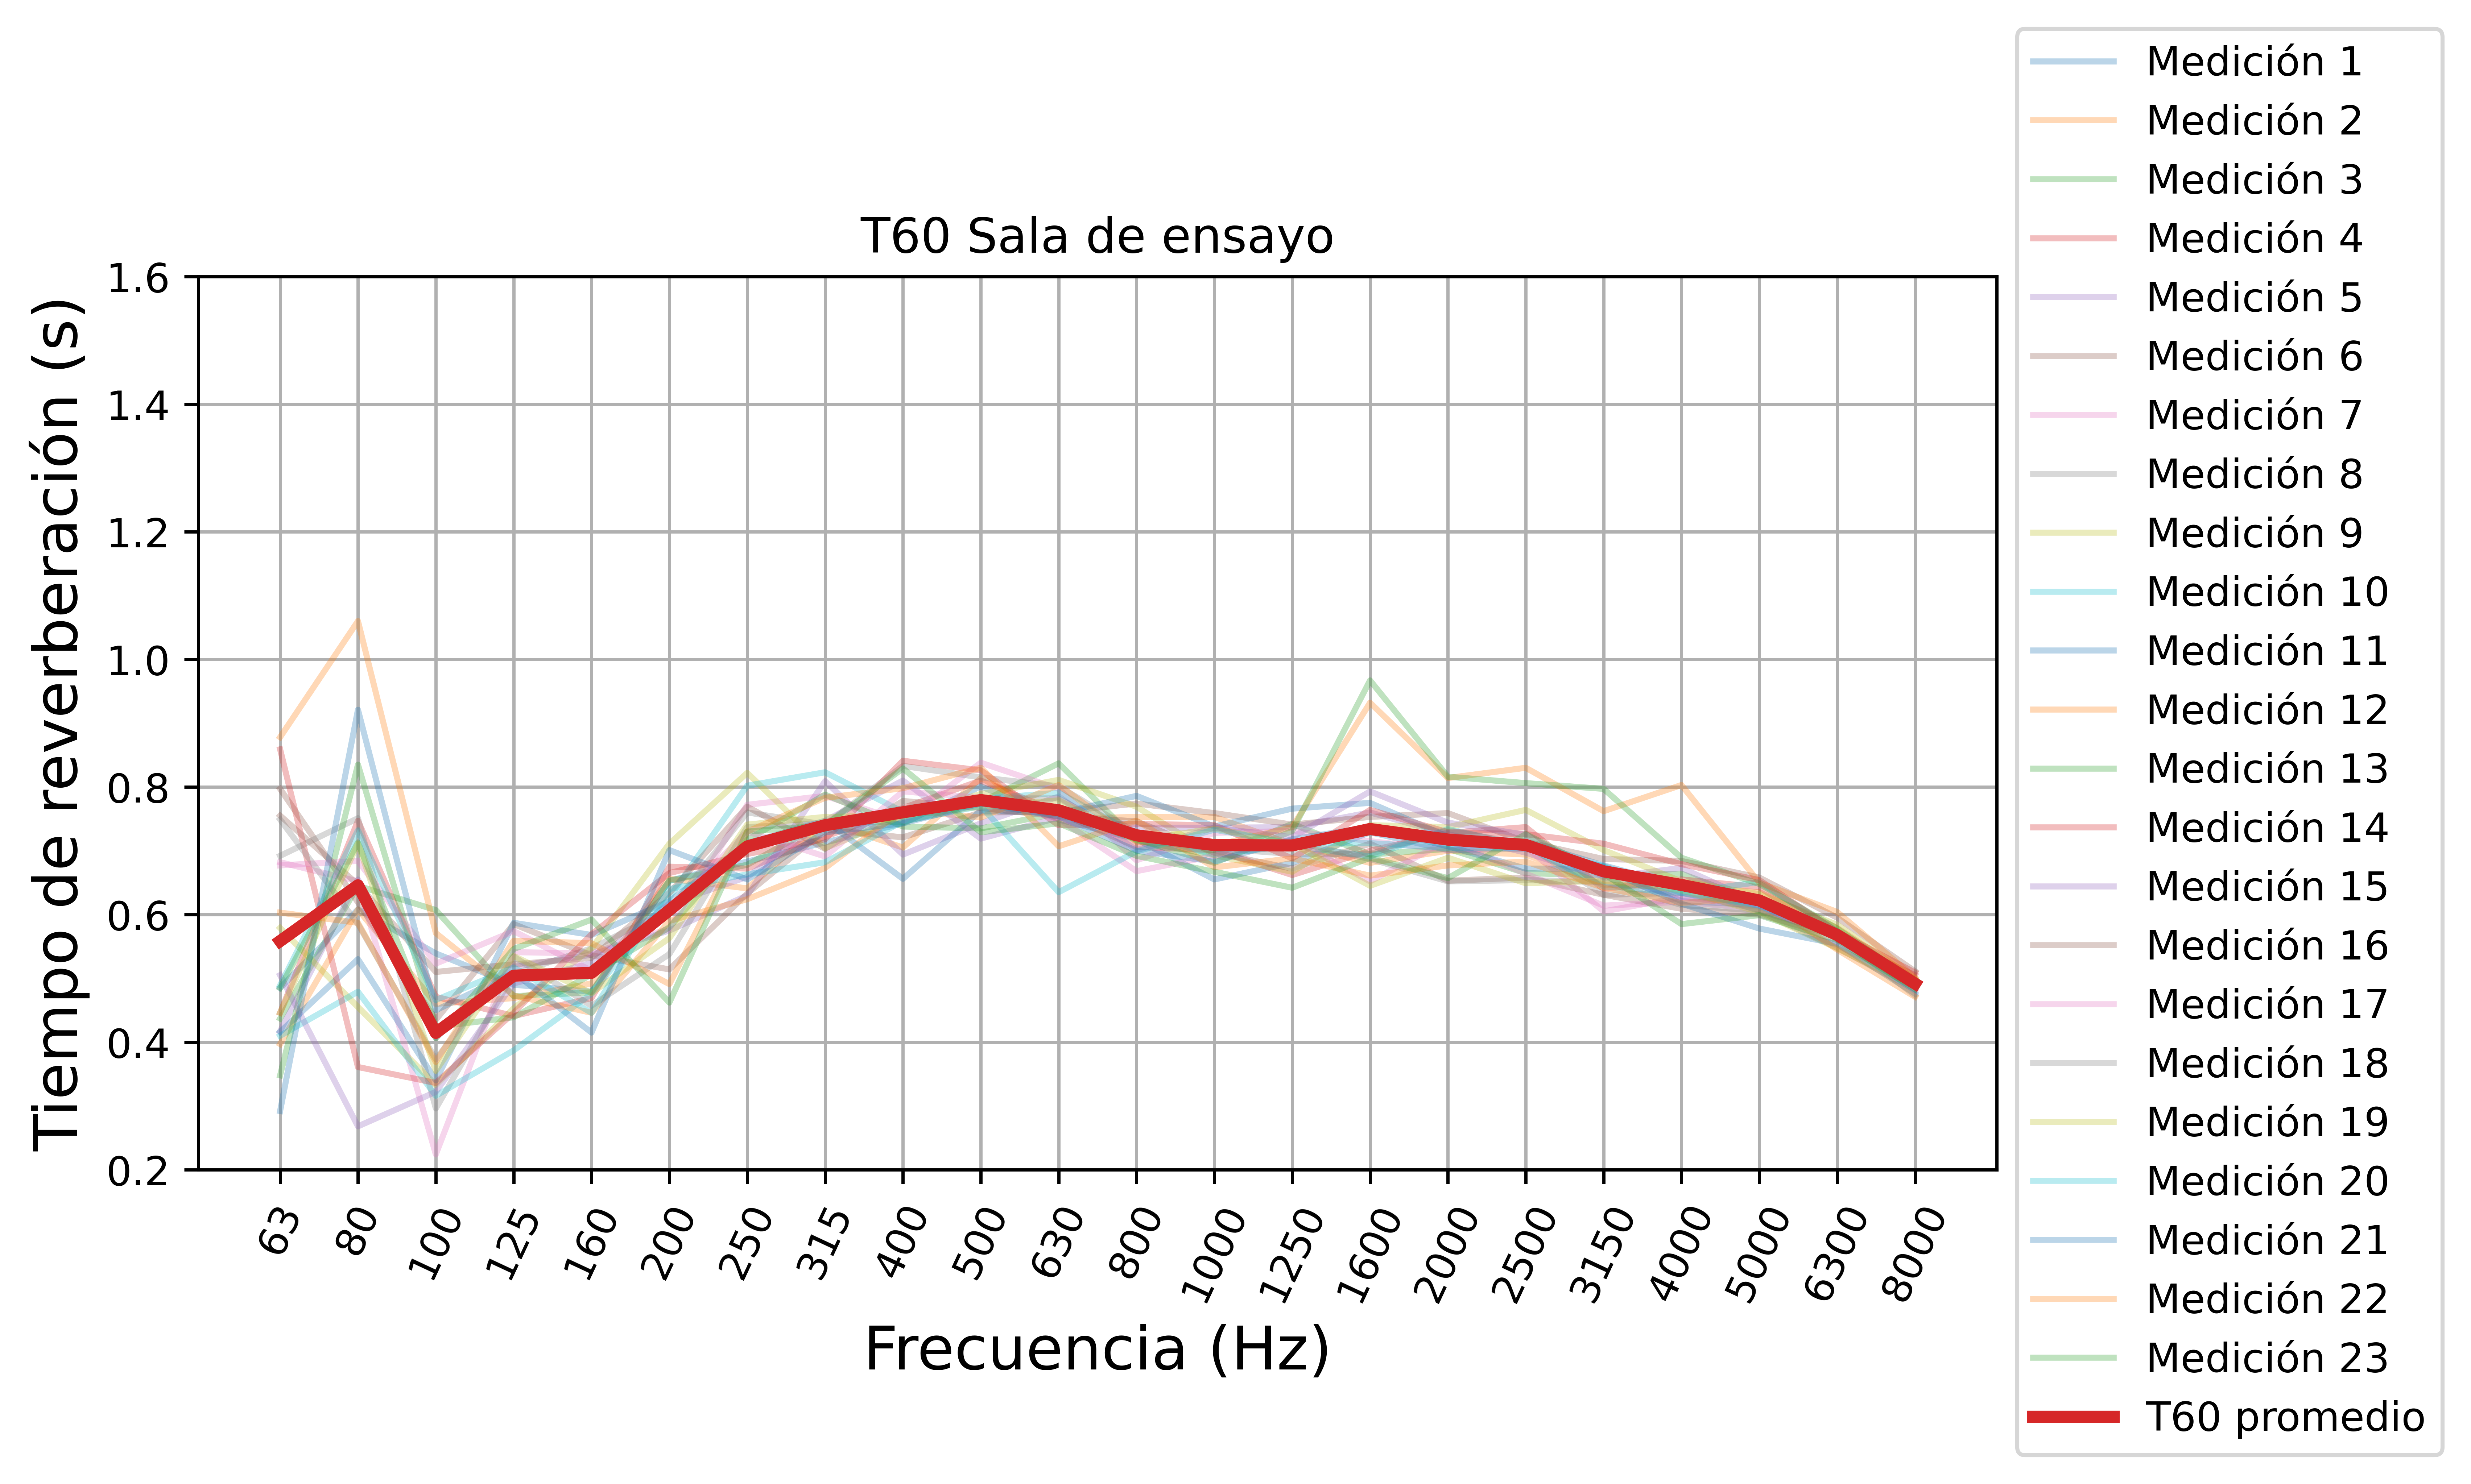
\includegraphics[width=10cm]{images/Tiempo de reverberación/T60_Sala_de_ensayo.png}
%         \caption{Tiempo de reverberación en sala de ensayo }
%         \label{fig:RT sala OCV}
%     \end{figure}
% \end{frame}
\begin{frame}{Tiempo de reverberación}
    \begin{figure}
        \centering
        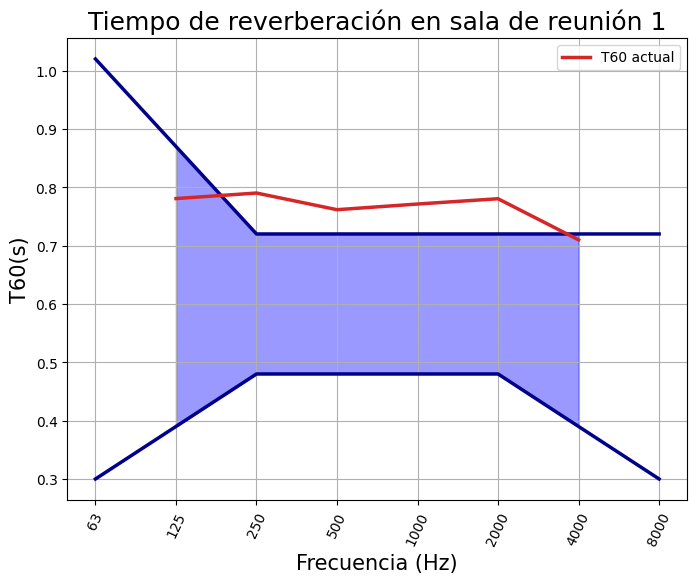
\includegraphics[width=7cm]{images/DIN/DIN sala reunion 1 actual.png}
        \caption{Tiempo de reverberación Sala de reunión 1}
        \label{fig:Ttarget sala de reunion 1}
    \end{figure}
\end{frame}
\begin{frame}{Tiempo de reverberación}
    \begin{figure}
        \centering
        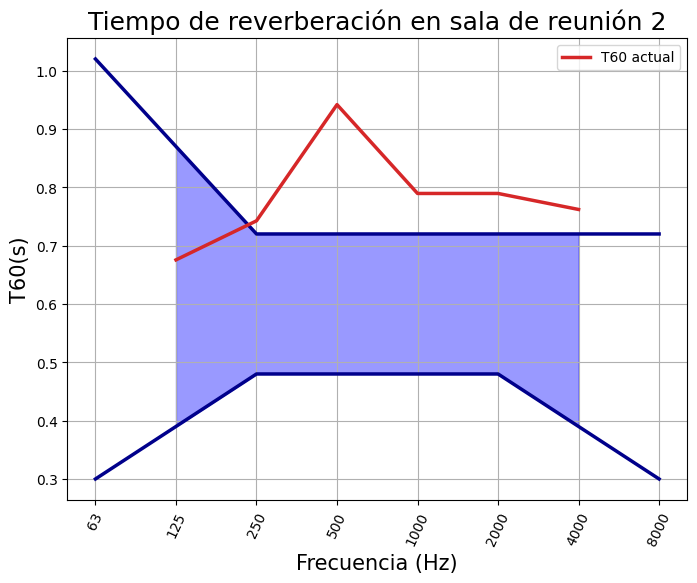
\includegraphics[width=7cm]{images/DIN/DIN sala reunion 2 actual.png}
        \caption{Tiempo de reverberación Sala de reunión 2}
        \label{fig:Ttarget sala de reunion 2}
    \end{figure}
\end{frame}

\begin{frame}{Tiempo de reverberación}
    \begin{figure}
        \centering
        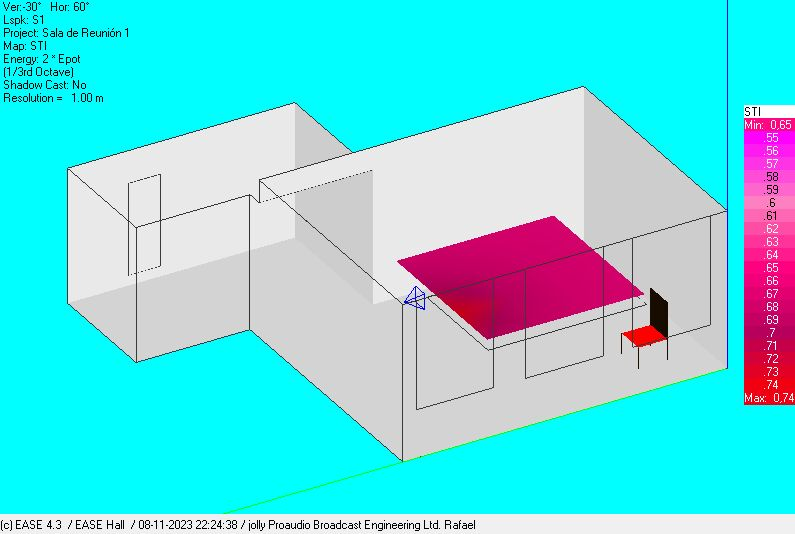
\includegraphics[width=7cm]{images/STI actual/STI_Reunion1_SinAcond.jpg}
        \caption{STI actual de Sala de reunión 1}
        \label{fig:STI actual sala reunion 1}
    \end{figure}
\end{frame}
\begin{frame}{Tiempo de reverberación}
    \begin{figure}
        \centering
        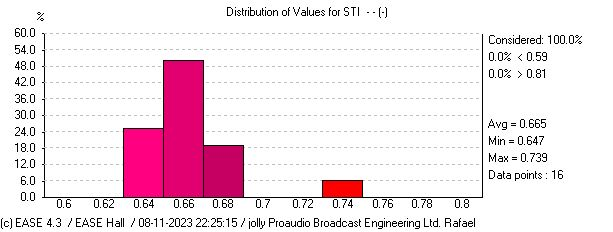
\includegraphics[width=7cm]{images/STI actual/STIdist_Reunion1_SinAcond.jpg}
        \caption{Distribución STI actual de Sala de reunión 1}
        \label{fig:distribución STI actual sala reunion 1}
    \end{figure}
\end{frame}

\begin{frame}{Tiempo de reverberación}
    \begin{figure}
        \centering
        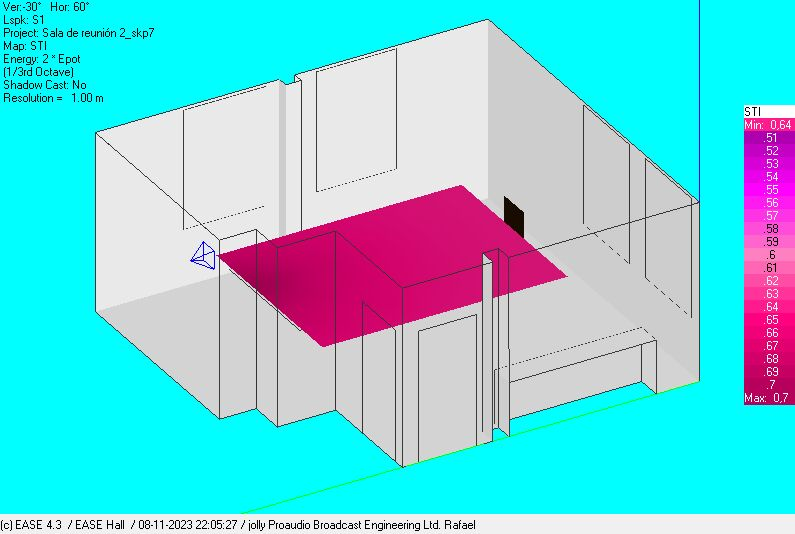
\includegraphics[width=7cm]{images/STI actual/STI_Reunion2_SinAcond.jpg}
        \caption{STI actual de Sala de reunión 2}
        \label{fig:STI actual sala reunion 2}
    \end{figure}
\end{frame}

\begin{frame}{Tiempo de reverberación}
    \begin{figure}
        \centering
        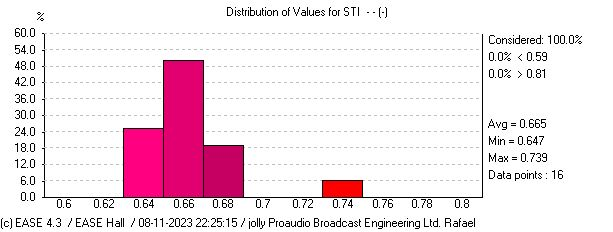
\includegraphics[width=7cm]{images/STI actual/STIdist_Reunion1_SinAcond.jpg}
        \caption{Distribución STI actual de Sala de reunión 2}
        \label{fig:distribución STI actual sala reunion 2}
    \end{figure}
\end{frame}

\begin{frame}{Tiempo de reverberación}
A partir de los valores obtenidos de tiempo de reverberación, se determinaron parámetros como claridad y definición, parámetros que se compararon con los recomendados en la siguiente tabla
     \begin{table}[H]
        \centering
        \caption{Parámetros acústicos de las salas de reunión y el estado}
        \label{tab: cumplimiento parametros RT de salas de reunión}
        \begin{tabular}{|l|c|c|c|}
        \hline
          \textbf{Parámetro}  & \textbf{Recomendación} & \textbf{Sala de reunión 1} & \textbf{Sala de reunión 2}\\ \hline
          $T_{target} (s)$ & 0.6 & \textcolor{red}{No cumple} & \textcolor{red}{No cumple}\\ \hline
          $C_{50speech}$ & $C_{50speech}>0$ & \textcolor{teal}{1.79} & \textcolor{teal}{0.89} \\ \hline
          STI& STI $>$ 0.45 & \textcolor{teal}{0.66} & \textcolor{teal}{0.64}\\\hline
        \end{tabular}
        
    \end{table}
\end{frame}
\begin{frame}{Tiempo de reverberación}
    También se determinó el parámetro de definición ($D_{50}$) para la sala de ensayo (ver figura \ref{fig: D50 sala de ensayo}), el cual esta fuera de lo recomendado.
    \begin{figure}[H]
        \centering
        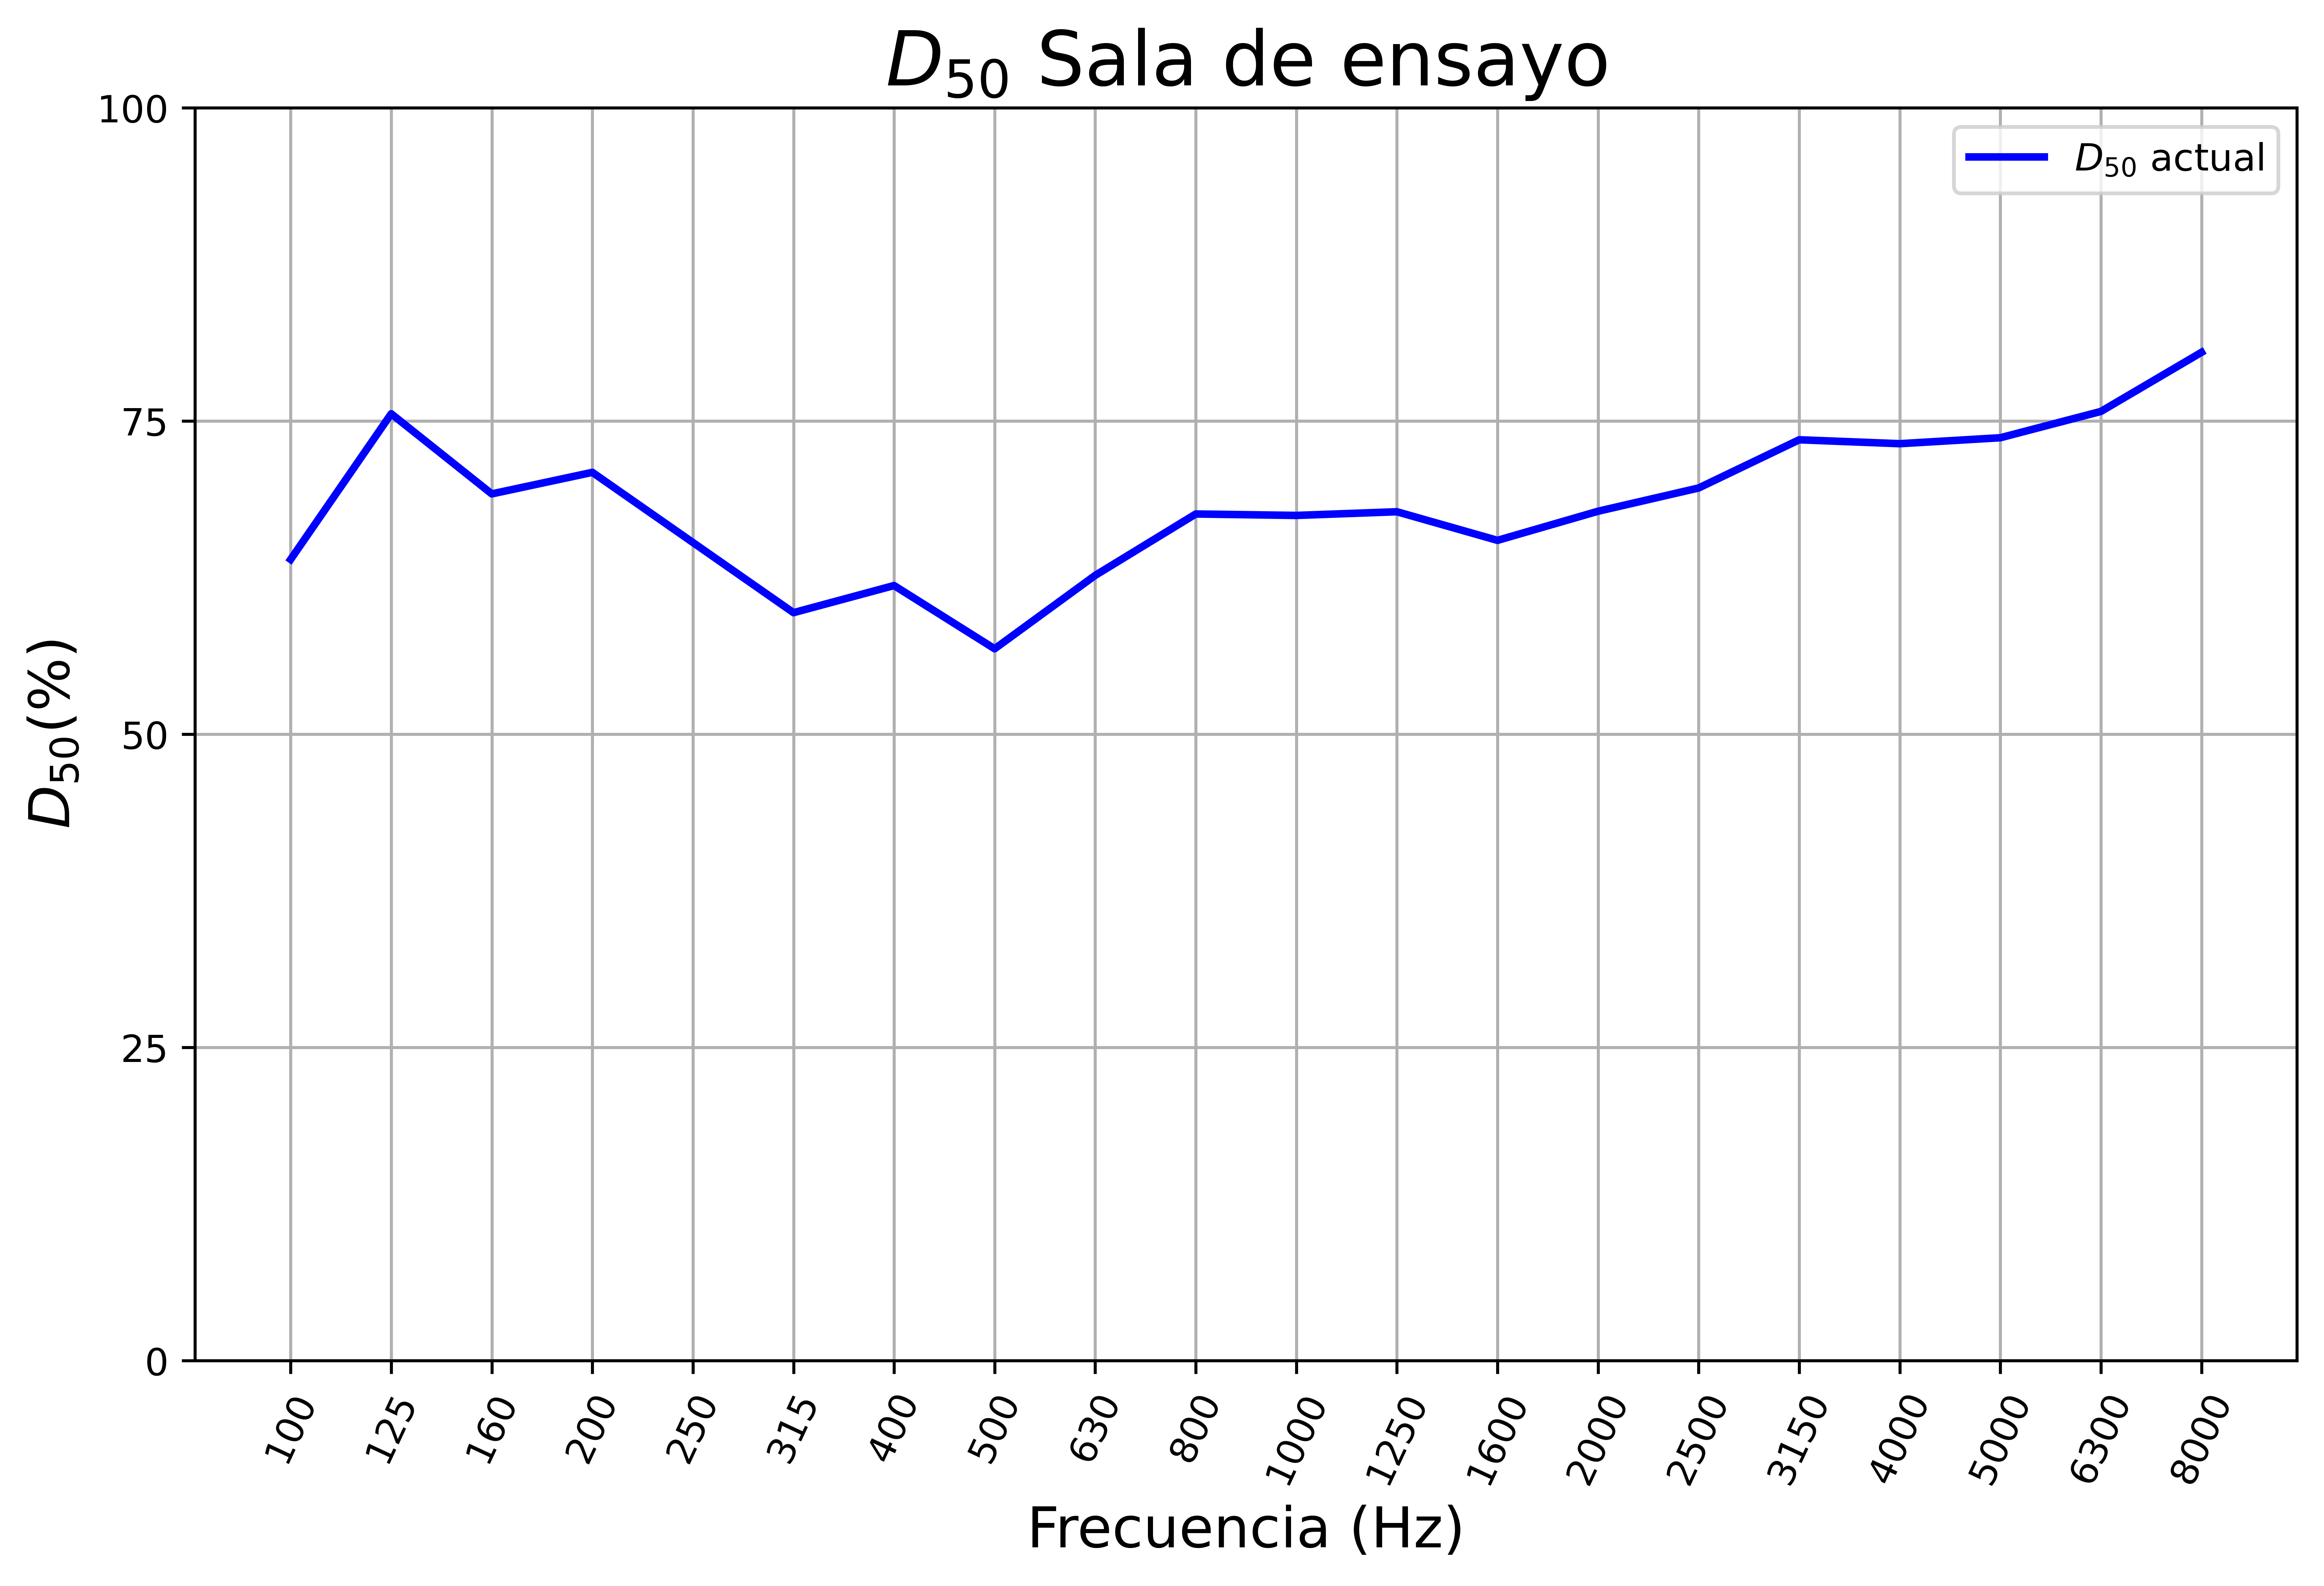
\includegraphics[scale=0.35]{images/D50_ensayo.png}
        \caption{$D_{50}$ de sala de ensayo}
        \label{fig: D50 sala de ensayo}
    \end{figure}
\end{frame}
\begin{frame}{Tiempo de reverberación}
    \begin{table}[H]
        \centering
        \begin{tabular}{|l|c|c|}
        \hline
        \textbf{Parámetro}& \textbf{Recomendación} & \textbf{Sala de ensayo}\\ \hline
        $RT{mid} (s)$&  0.74 & \textcolor{red}{0.74} \\ \hline
        $C_{80}$ & $-2<C_{80}<2$ & \textcolor{red}{6.04} \\\hline
        $D_{50}$ & $D_{50}<$ 0.5 & \textcolor{red}{No cumple} \\\hline
        \end{tabular}
        \caption{Parámetros acústicos de la sala de ensayo y su estado}
        \label{tab:prametros acusticos sala ensayo}
    \end{table}
\end{frame}

\section{Modelación}
\begin{frame}{Modelo SketchUp}
    \begin{figure}
        \centering
        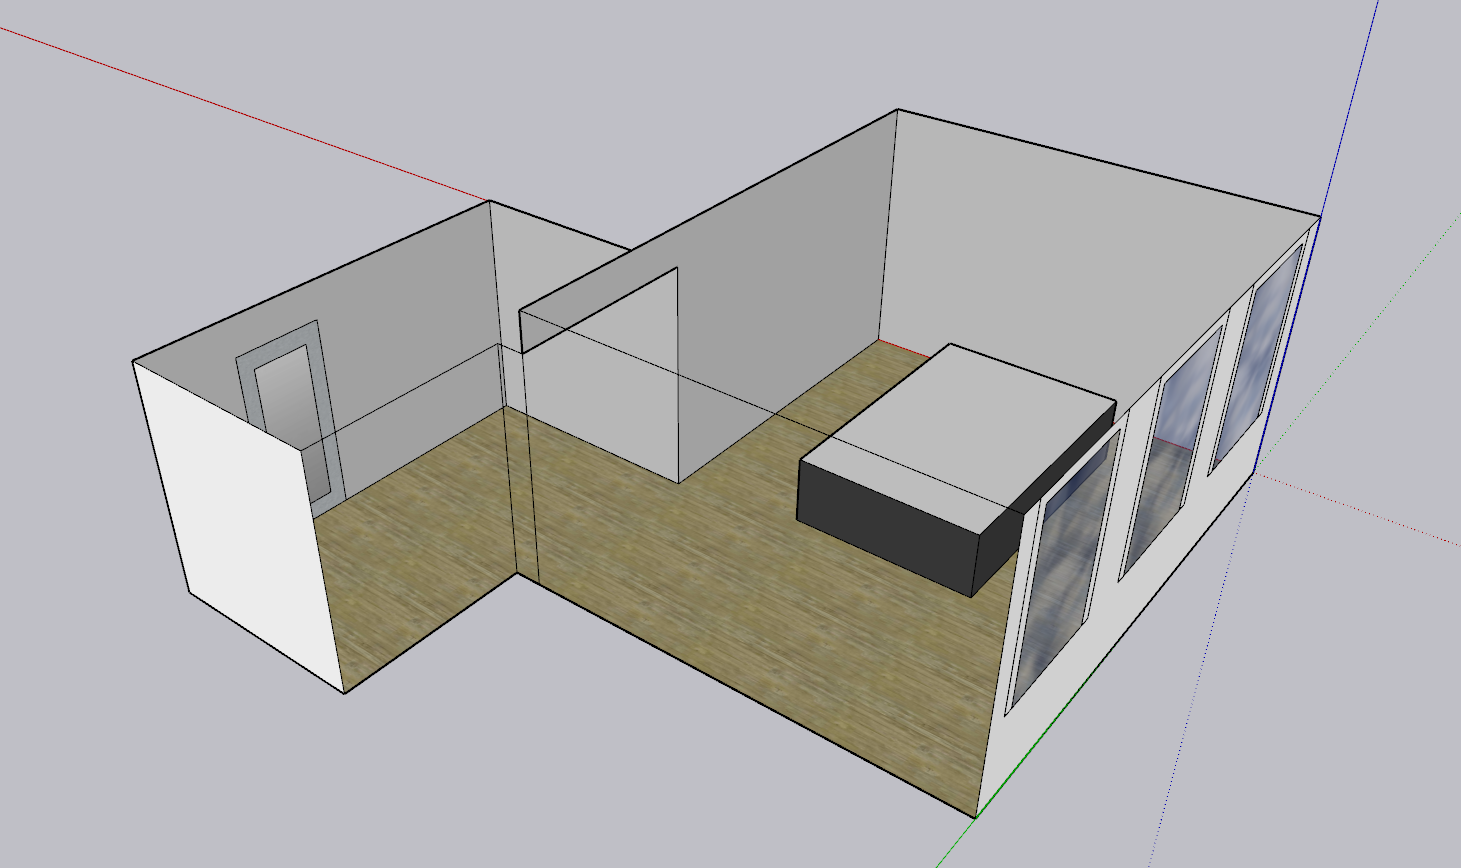
\includegraphics[width=10cm]{images/Sketchup/Sala 1 Sketchup.png}
        \caption{Modelo en SketchUp sala de reunión 1}
        \label{fig:skp sala 1}
    \end{figure}
\end{frame}

\begin{frame}{Modelo SketchUp}
    \begin{figure}
        \centering
        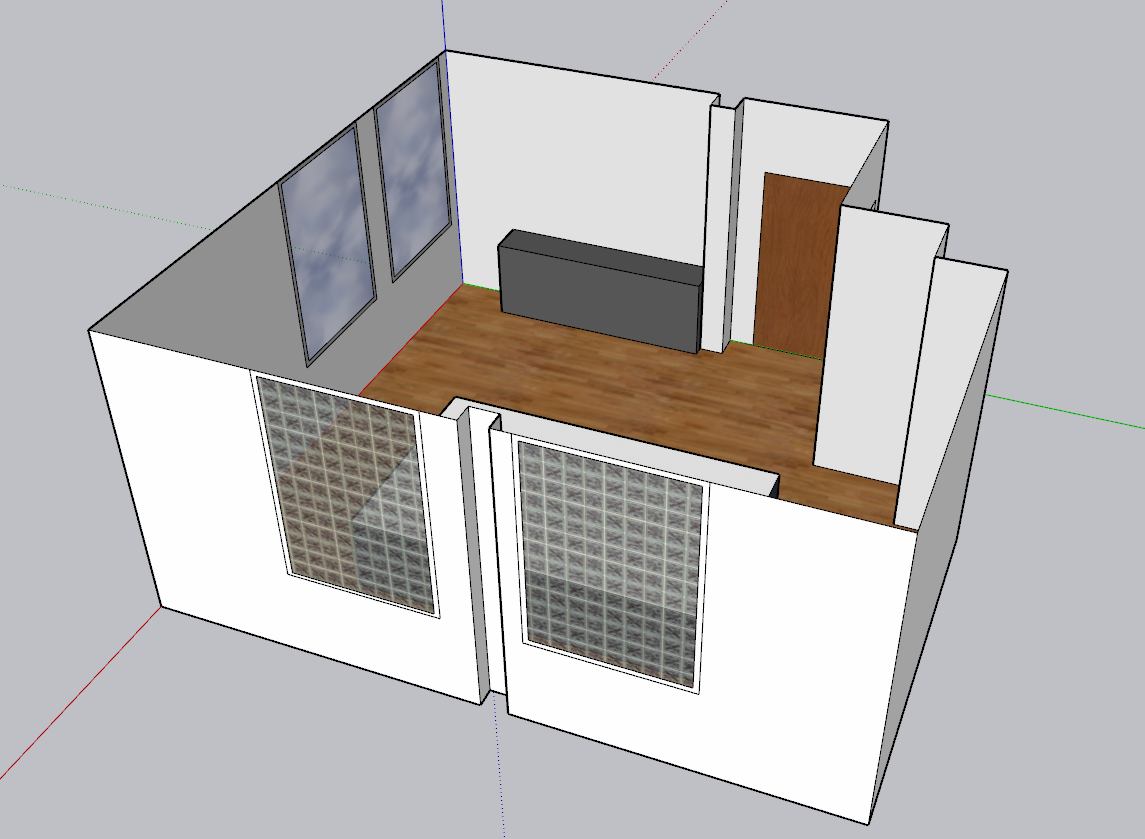
\includegraphics[width=8cm]{images/Sketchup/Sala 2 Sketchup.png}
        \caption{Modelo en SketchUp sala de reunión 2}
        \label{fig:skp sala 2}
    \end{figure}
\end{frame}

\begin{frame}{Modelo SketchUp}
    \begin{figure}
        \centering
        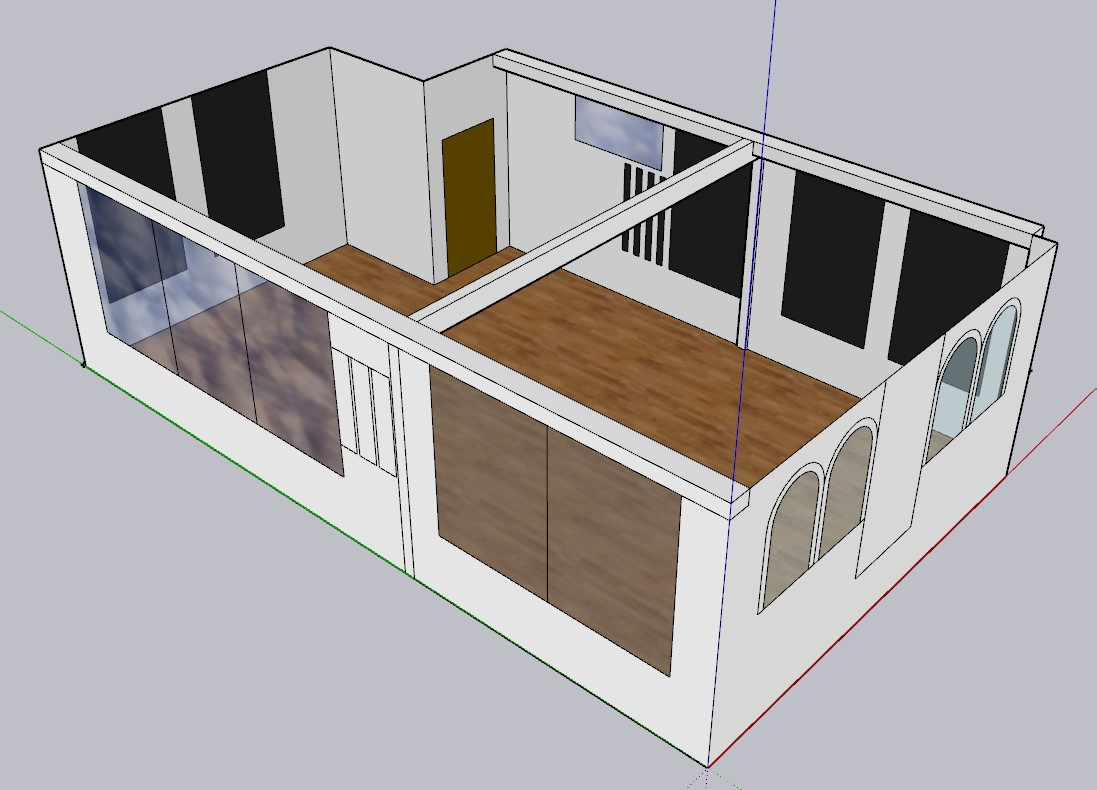
\includegraphics[width=8cm]{images/Sketchup/Sala ensayo Sketchup.jpg}
        \caption{Modelo en SketchUp sala de ensayo}
        \label{fig:skp sala ensayo}
    \end{figure}
\end{frame}

\begin{frame}{Análisis modal}
    Comportamiento modal de sala de ensayo
    \begin{figure}
        \centering
        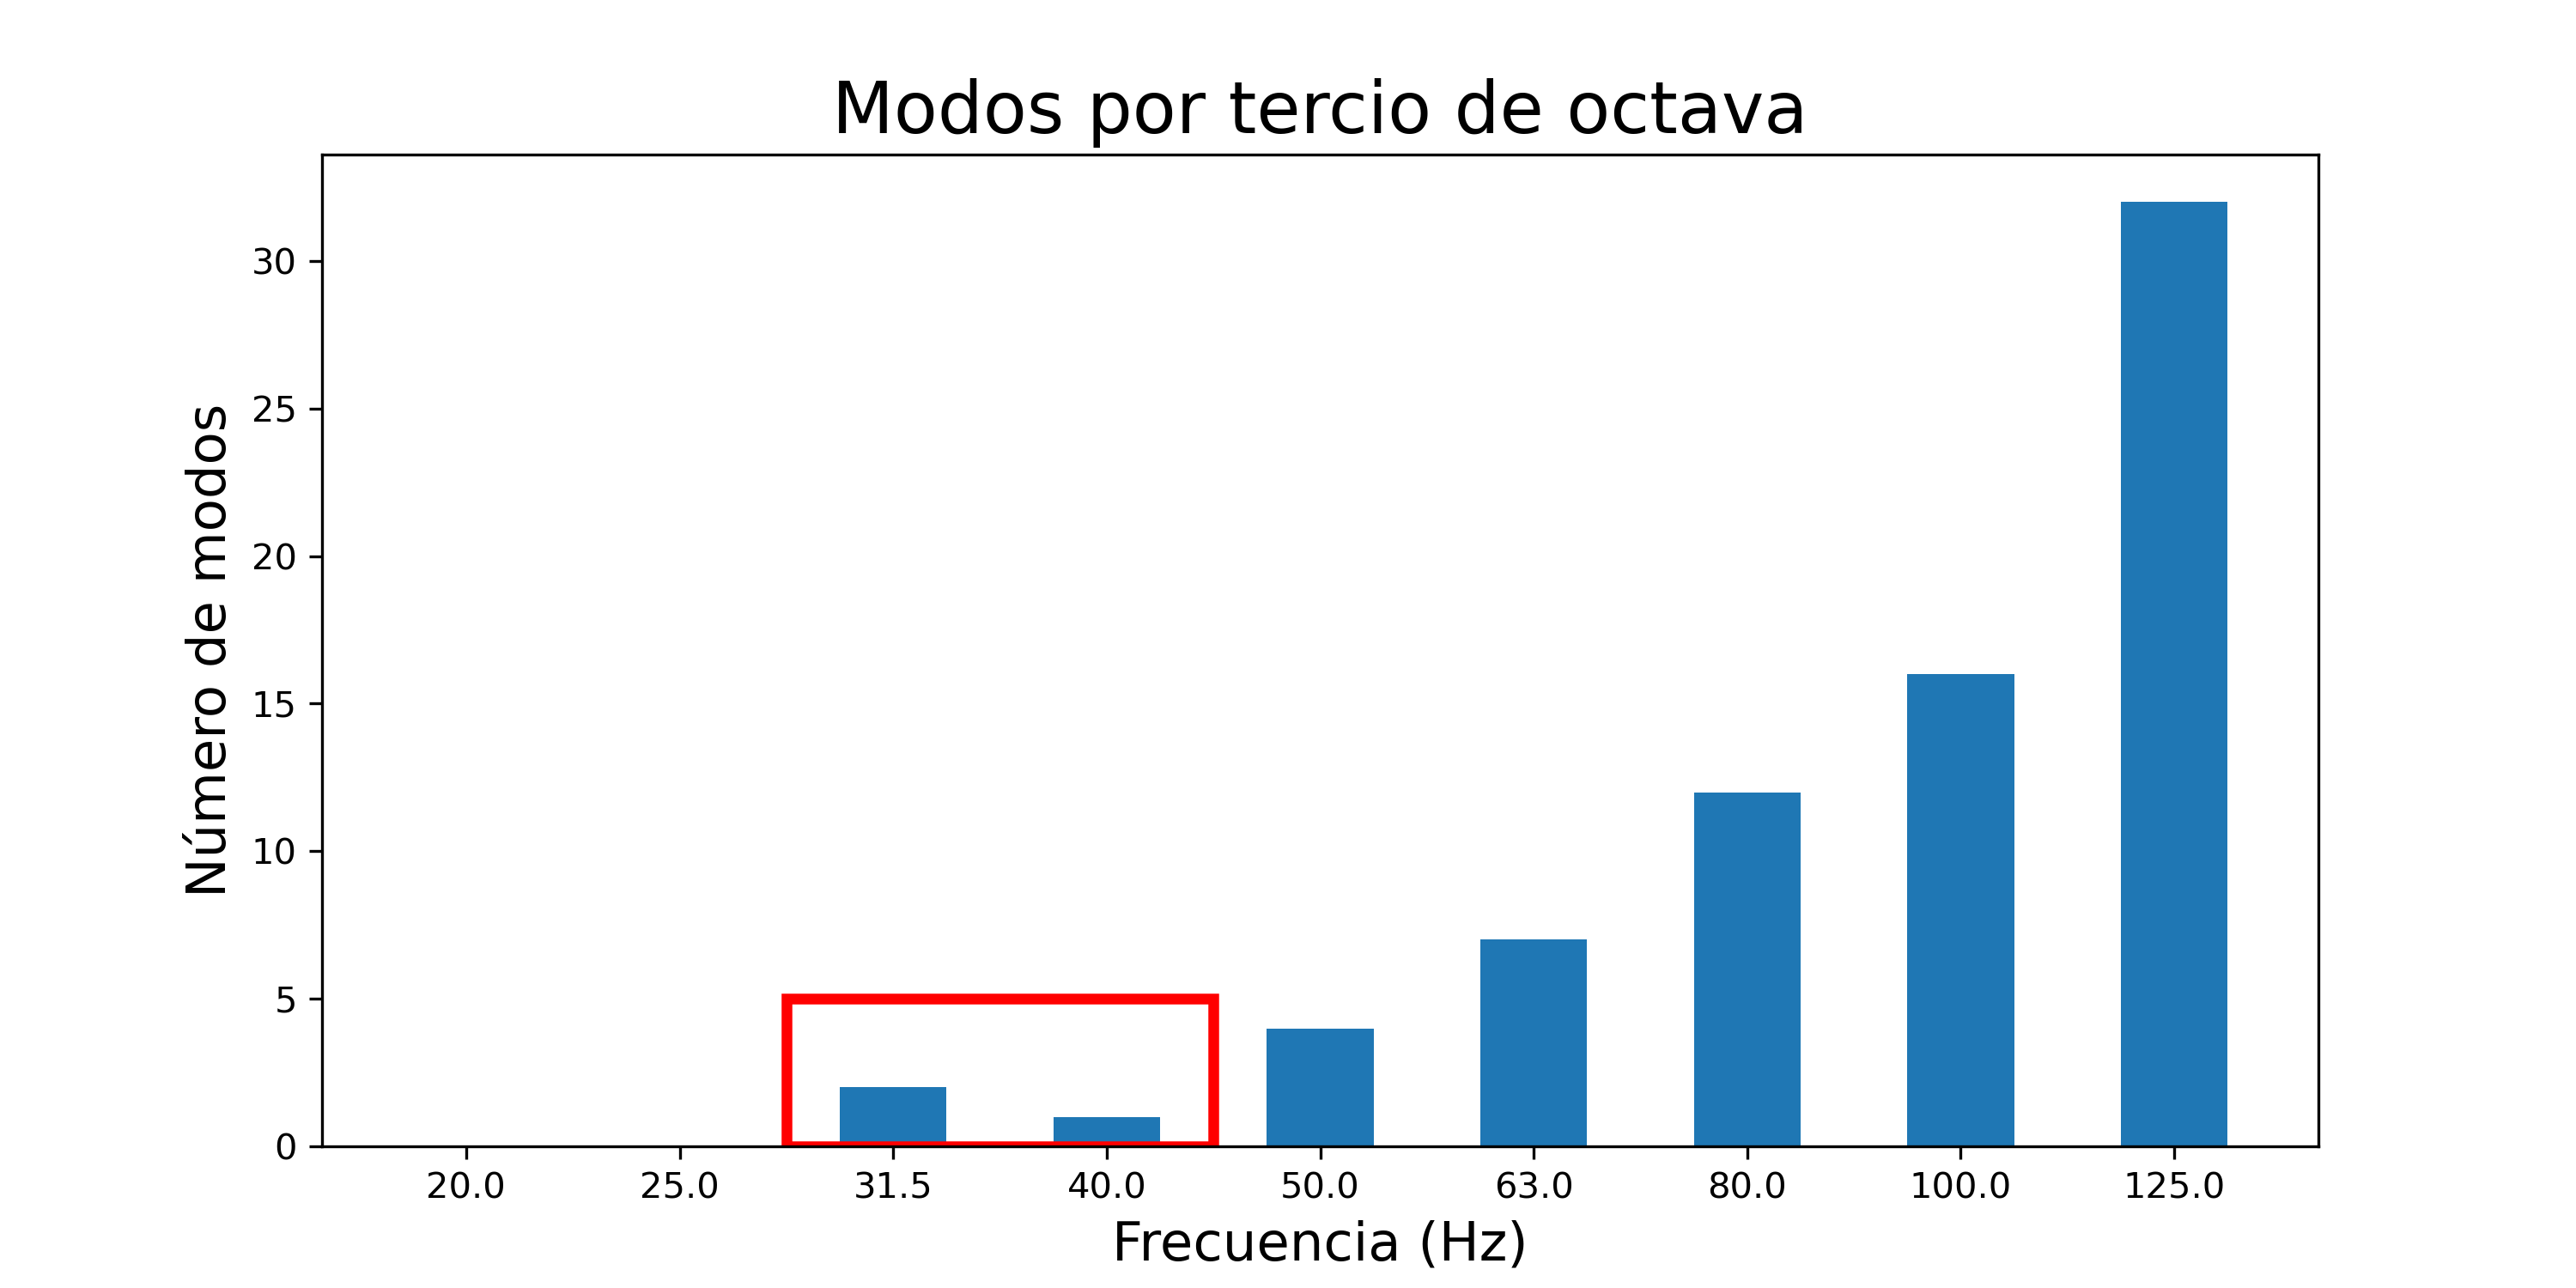
\includegraphics[width=8cm]{images/Modos/densidad modal.png}
        \caption{Densidad modal de sala de ensayo}
        \label{fig:densidad modal}
    \end{figure}
\end{frame}
\begin{frame}{Análisis modal}
    \begin{figure}
        \centering
        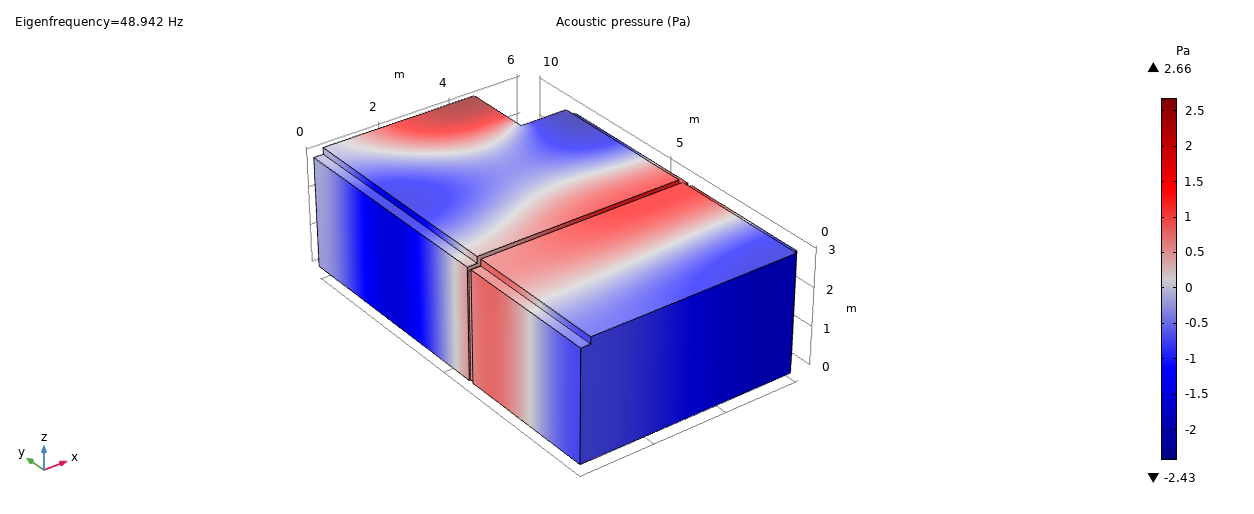
\includegraphics[width=8cm]{images/Modos/modo_48hz.png}
        \caption{Modo en sala de ensayo}
        \label{fig:modo 48 hz}
    \end{figure}
\end{frame}
\begin{frame}{Análisis modal}

\begin{figure}[H]
    \centering
    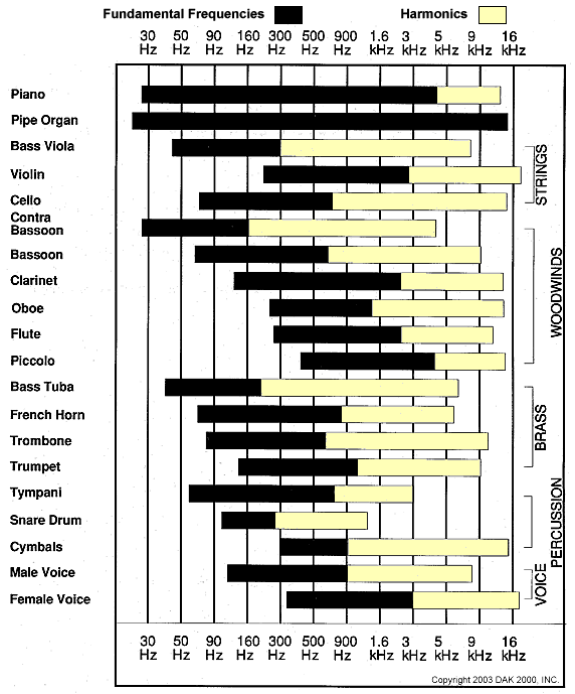
\includegraphics[scale=0.5]{images/Modos/RangoInstrumentos.png}
    \caption{Rango en frecuencia de instrumentos musicales}
    \label{fig:RangoInstrumentos}
\end{figure}
\end{frame}


\begin{frame}{Modelo EASE}
Los modelos en SketchUp correspondientes, se importaron en el software EASE y se ingresó la materialidad respectiva a cada superficie, con información de coeficientes de absorción encontrados en la literatura, como se ve en la siguiente tabla:
    \begin{table}[H]
        \centering
        \caption{Materiales utilizados para modelo en EASE.}
        \label{tab:materiales-ease}
        \begin{tabular}{|c|cccccc|c|}
        \hline
        \multirow{2}{*}{\textbf{Material}} & \multicolumn{6}{c|}{\textbf{Frecuencia (Hz)}}                                                                          & \multirow{2}{*}{\textbf{Fuente}} \\ \cline{2-7} 
                & \multicolumn{1}{c|}{125} & \multicolumn{1}{c|}{250} & \multicolumn{1}{c|}{500} & \multicolumn{1}{c|}{1000} & \multicolumn{1}{c|}{2000} & 4000 & \\ \hline
        Parquet & \multicolumn{1}{c|}{0.04} & \multicolumn{1}{c|}{0.04} & \multicolumn{1}{c|}{0.07} & \multicolumn{1}{c|}{0.06} & \multicolumn{1}{c|}{0.06} &  0.07 & Recuero\\ \hline
        Madera  & \multicolumn{1}{c|}{0.25} & \multicolumn{1}{c|}{0.34} & \multicolumn{1}{c|}{0.18} & \multicolumn{1}{c|}{0.10} & \multicolumn{1}{c|}{0.10} &  0.06 & Recuero\\  \hline
        Black Acoustic Board (2") & \multicolumn{1}{c|}{0.13} & \multicolumn{1}{c|}{0.75} & \multicolumn{1}{c|}{1} & \multicolumn{1}{c|}{1} & \multicolumn{1}{c|}{1} & 1 & Blackboard\\ \hline
        Vidrio  & \multicolumn{1}{c|}{0.05} & \multicolumn{1}{c|}{0.50} & \multicolumn{1}{c|}{0.03} & \multicolumn{1}{c|}{0.03} & \multicolumn{1}{c|}{0.02} & 0.02 & Recuero\\ \hline
        \end{tabular}
    \end{table}
\end{frame}
\begin{frame}{Modelo EASE con ocupación}
    \noindent Para tener modelar la sala ocupada se consideró el siguiente coeficiente de absorción por persona:
    \begin{table}[H]
        \centering
        \caption{Coeficiente de absorción de una persona sentada de EASE}
        \label{tab: coef abs persona}
        \begin{tabular}{|l|l|l|l|l|l|l|}
        \hline
        \textbf{Frecuencia Hz}      & 125  & 250  & 500  & 1000 & 2000 & 4000 \\ \hline
        \textbf{Absorción $\alpha$} & 0.31 & 0.51 & 0.73 & 0.80 & 0.82 & 0.82 \\ \hline
        \end{tabular}
    \end{table}
\end{frame}
\begin{frame}{Distribución de músicos en ensayo}
    \begin{figure}
        \centering
        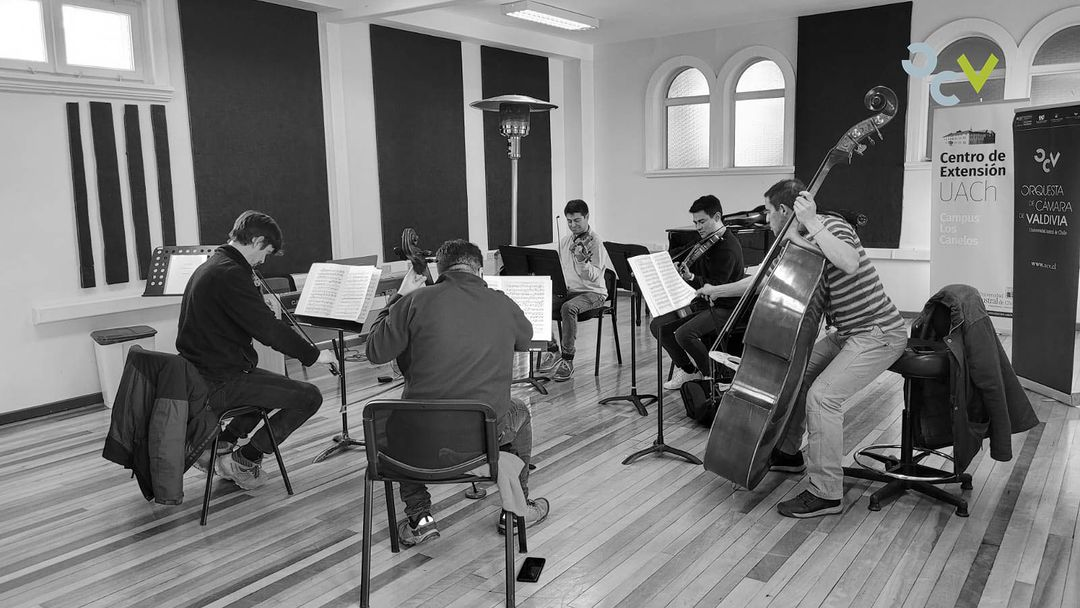
\includegraphics[width=8cm]{images/OCV/OCV cuerdas.jpg}
        \caption{Distribución de músicos de cuerdas frotadas en ensayo}
    \end{figure}
\end{frame}
\begin{frame}{Distribución de músicos en ensayo}
    \begin{figure}
        \centering
        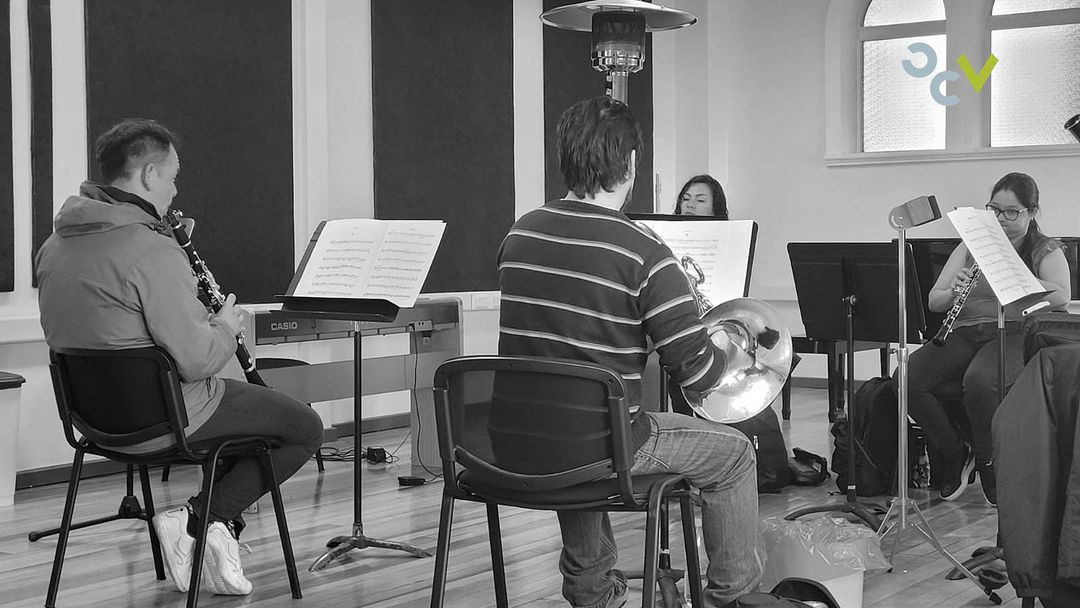
\includegraphics[width=8cm]{images/OCV/OCV vientos.jpg}
        \caption{Distribución de músicos de instrumentos de bronce y madera en ensayo}
    \end{figure}
\end{frame}
\begin{frame}{Distribución de músicos en salon EASE}
    \begin{figure}
        \centering
        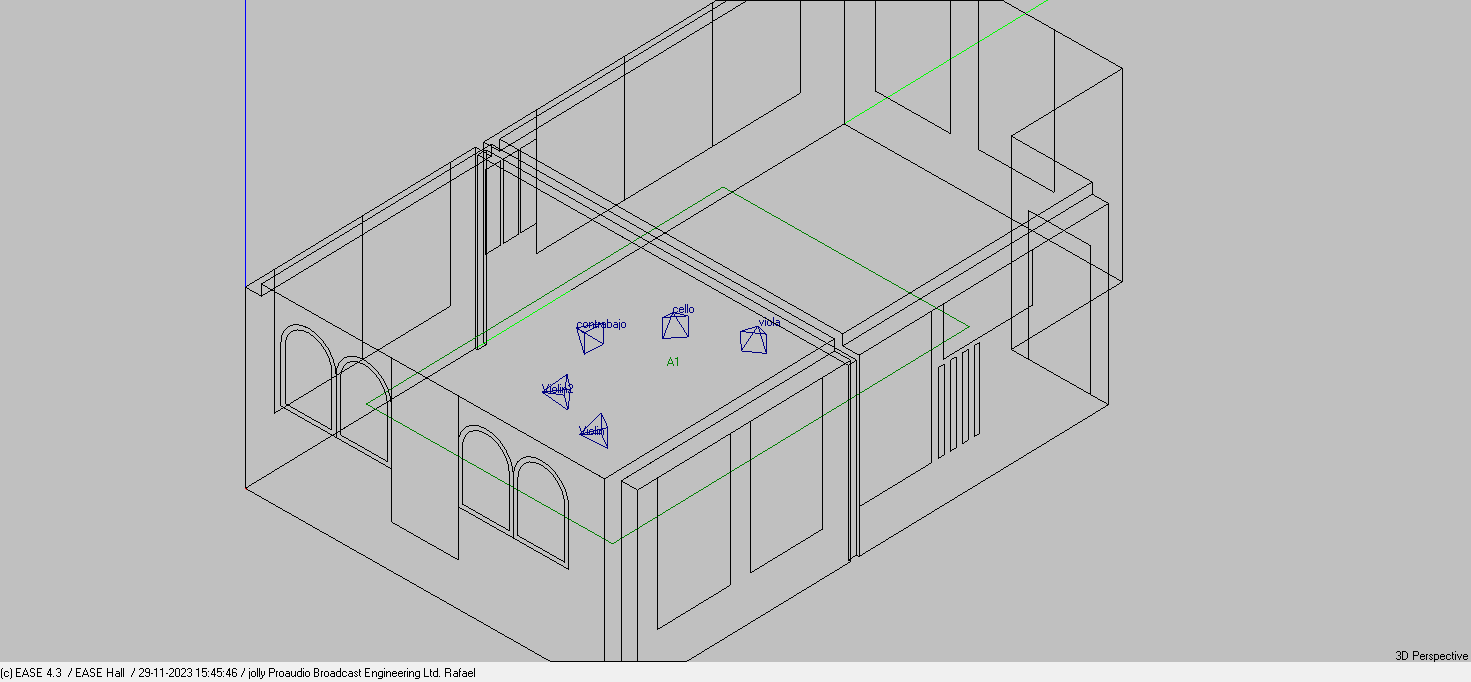
\includegraphics[width=8cm]{images/Sketchup/Instrumentos_ease.png}
        \caption{Distribución de músicos en sala de ensayo EASE}
    \end{figure}
\end{frame}
\section{Propuesta}
\begin{frame}{Sala de reuniones}
    Para las salas de reuniones se seleccionó el siguiente material.
    \begin{figure}
        \centering
        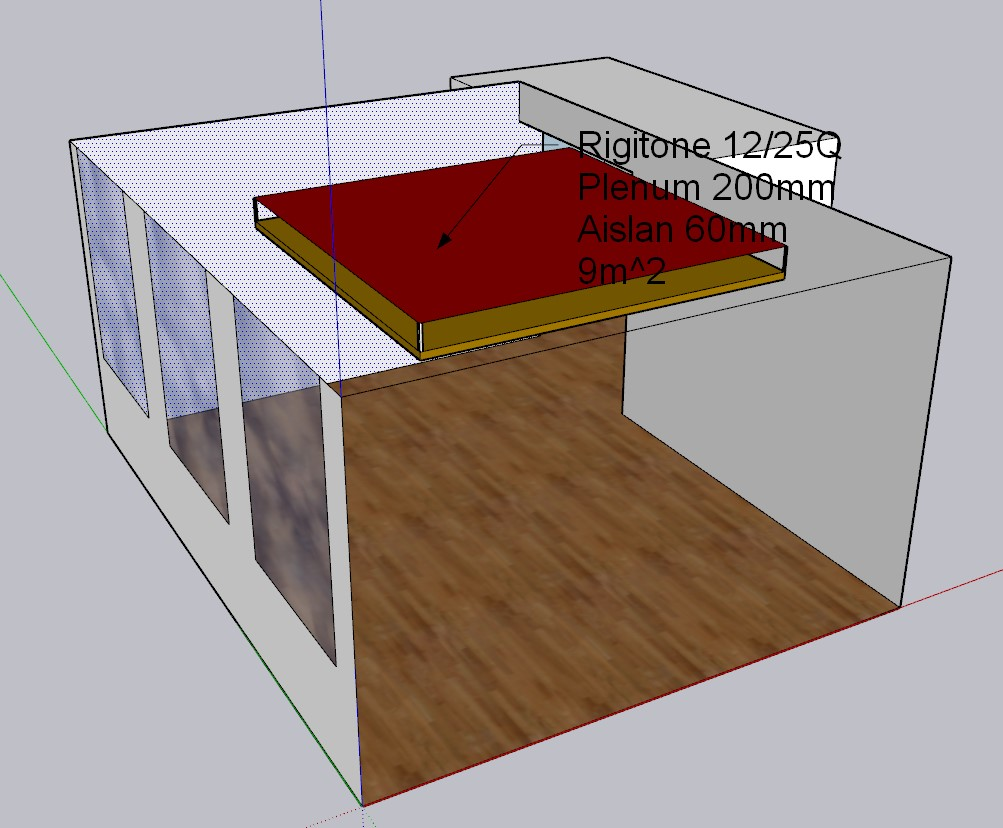
\includegraphics[width=6cm]{images/Propuesta/propuesta_reunion1.jpg}
        \caption{Modelo SketchUp de sala de reunión 1 acondicionado}
        \label{fig:modelo sketchup sala 1 acond}
    \end{figure}
\end{frame}
\begin{frame}{Sala de reuniones}
    \begin{figure}
        \centering
        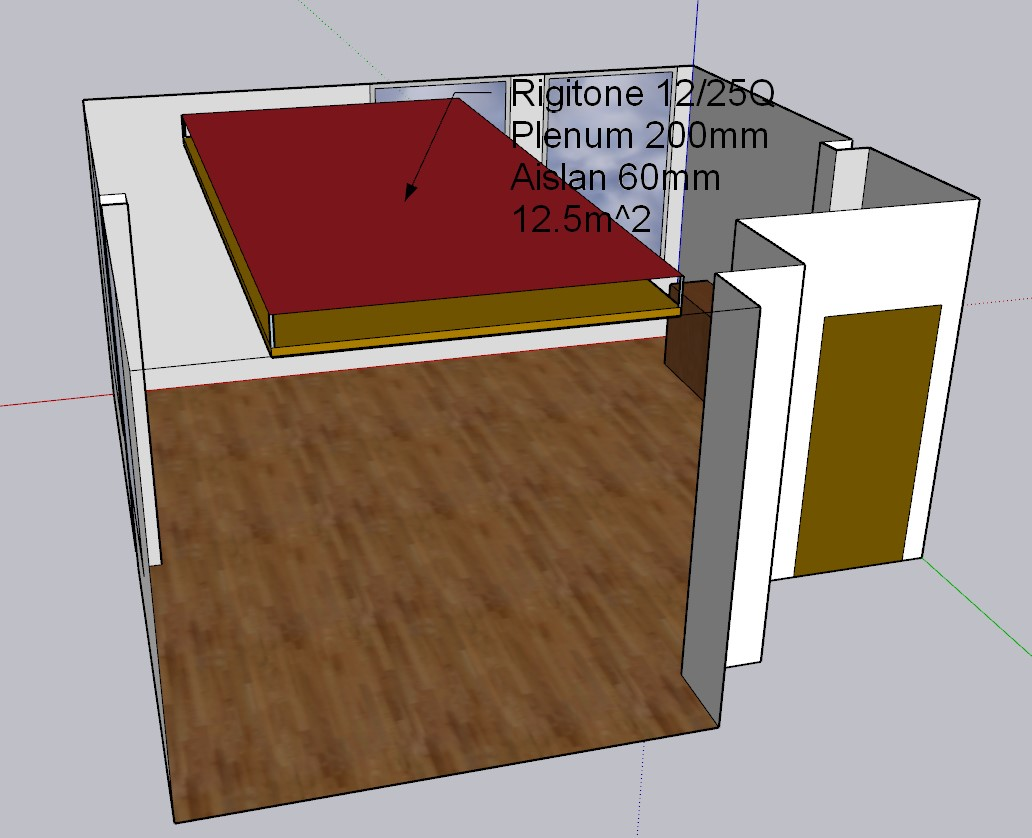
\includegraphics[width=6cm]{images/Propuesta/propuesta_reunion2.jpg}
        \caption{Modelo SketchUp de sala de reunión 2 acondicionado}
        \label{fig:modelo sketchup sala 2 acond}
    \end{figure}
    
\end{frame}
\begin{frame}{Sala de reuniones}
    \begin{figure}[H]
        \centering
        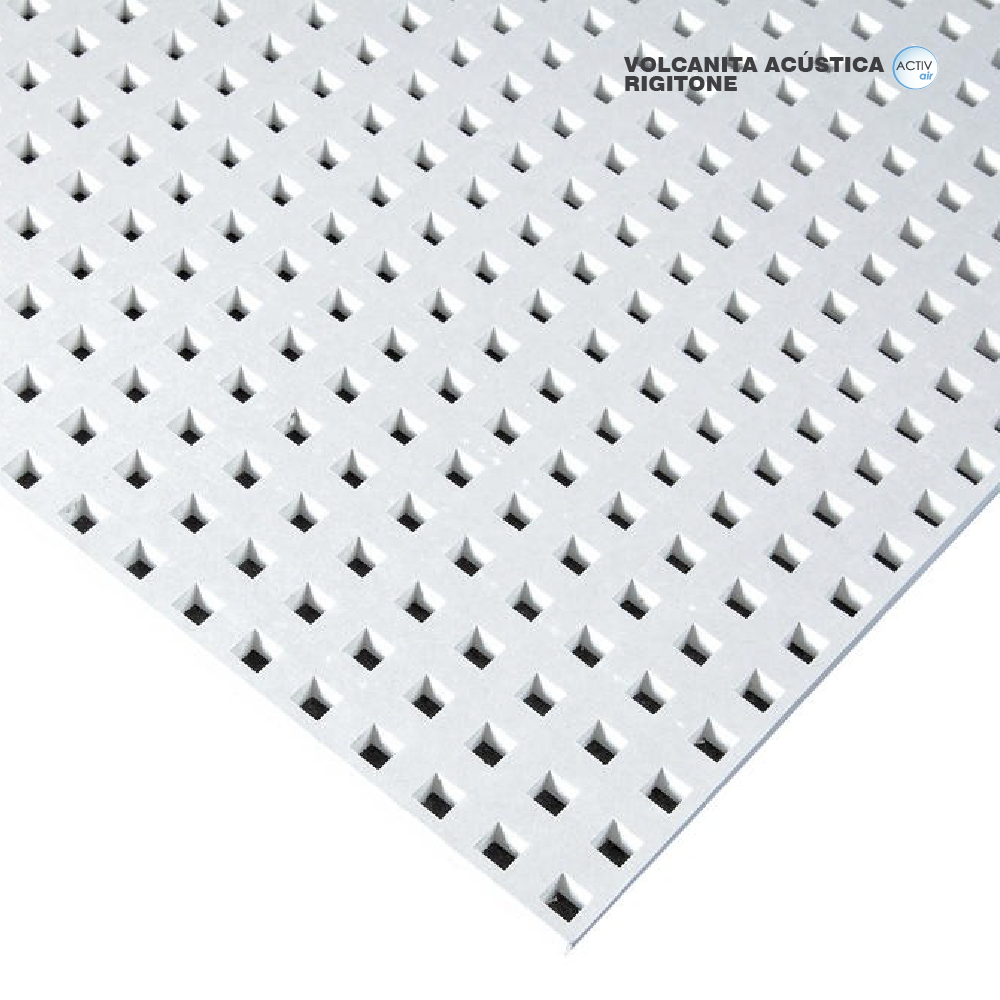
\includegraphics[width=6cm]{images/Propuesta/Rigitone-12-25Q.png}
        \caption{Material escogido para acondicionar salas de reunión}
        \label{fig:material escogido para acond salas de reunion}
    \end{figure}
\end{frame}
\begin{frame}{Sala de reuniones}
    \begin{table}[H]
    \centering
    \begin{tabular}{|lllllll|}
    \hline
    \multicolumn{7}{|c|}{\textbf{12/25 Q}} \\ \hline
    \multicolumn{1}{|l|}{Plenum} & \multicolumn{6}{c|}{200 mm} \\ \hline
    \multicolumn{1}{|l|}{Aislan} & \multicolumn{6}{c|}{60  mm} \\ \hline
    \multicolumn{1}{|l|}{Frecuencia Hz} & \multicolumn{1}{l|}{125 Hz} & \multicolumn{1}{l|}{250 Hz} & \multicolumn{1}{l|}{500 Hz} & \multicolumn{1}{l|}{1 KHz} & \multicolumn{1}{l|}{2 KHz} & 4 KHz \\ \hline
    \multicolumn{1}{|l|}{$\alpha$} & \multicolumn{1}{l|}{0.60} & \multicolumn{1}{l|}{0.90} & \multicolumn{1}{l|}{0.95} & \multicolumn{1}{l|}{0.90} & \multicolumn{1}{l|}{0.80} & 0.75 \\ \hline
    \end{tabular}
    \caption{Coeficiente de absorción de Volcanita acústica Rigitone}
    \end{table}  

\end{frame}
\begin{frame}{Sala de ensayo}
    \begin{figure}[H]
        \centering
        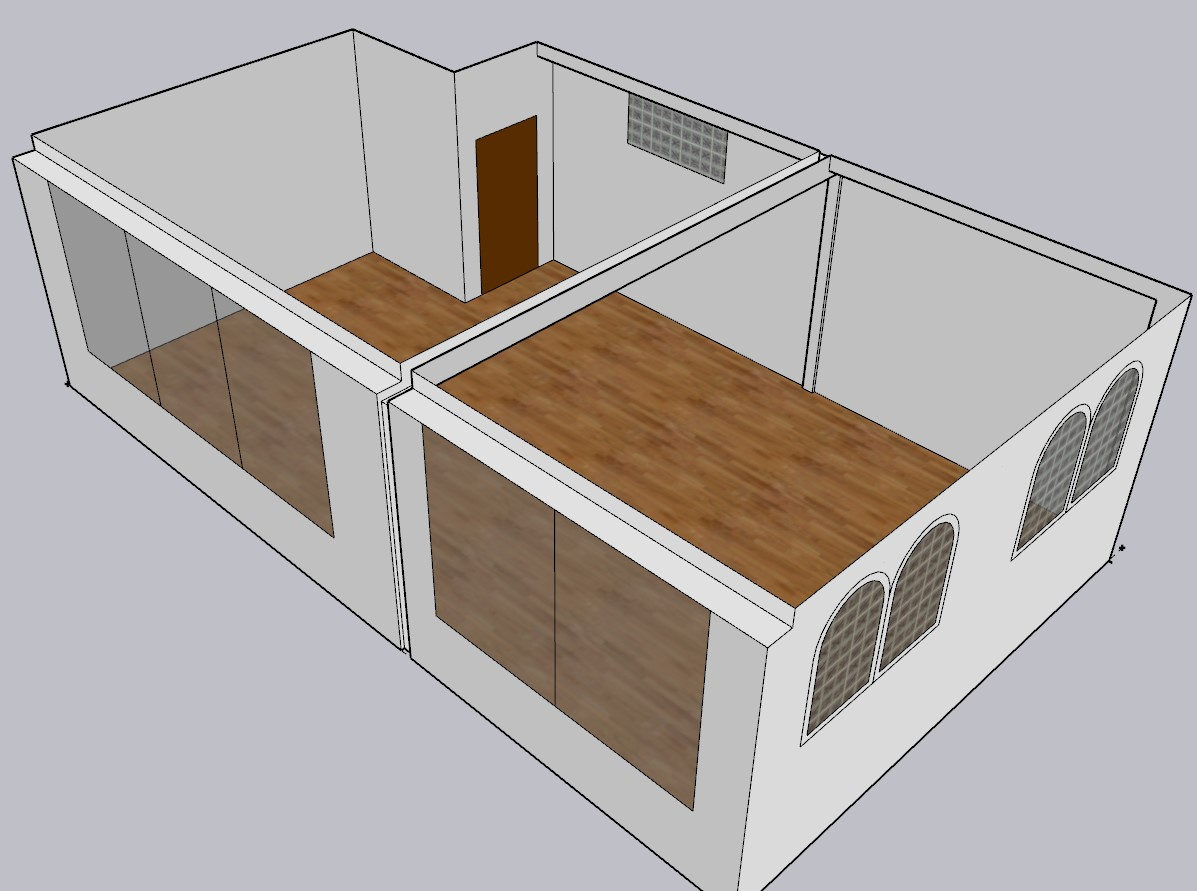
\includegraphics[width=6cm]{images/Propuesta/Sala ensayo sin paneles.jpg}
        \caption{Modelo SketchUp de sala de ensayo sin paneles}
    \end{figure}
\end{frame}
\begin{frame}{Resultados salas de reuniones}
    \begin{figure}
        \centering
        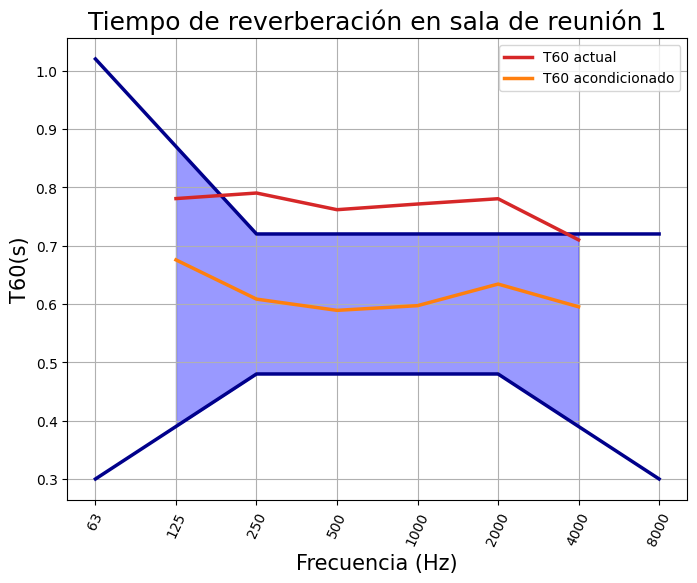
\includegraphics[width=7cm]{images/DIN/DIN sala reunion 1 comparacion.png}
        \caption{Tiempo de reverberación de sala de reunión 1 acondicionado}
        \label{fig:din sala 1 acond}
    \end{figure}
\end{frame}
\begin{frame}{Resultados salas de reuniones}
    \begin{figure}
        \centering
        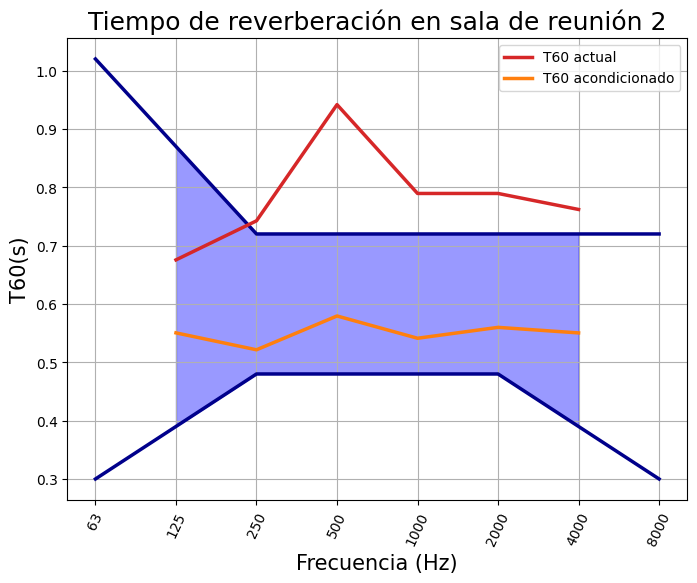
\includegraphics[width=7cm]{images/DIN/DIN sala reunion 2 comparacion.png}
        \caption{Tiempo de reverberación de sala de reunión 2 acondicionado}
        \label{fig:din sala 2 acond}
    \end{figure}
\end{frame}

\begin{frame}{Resultados salas de reuniones}
    \begin{figure}
        \centering
        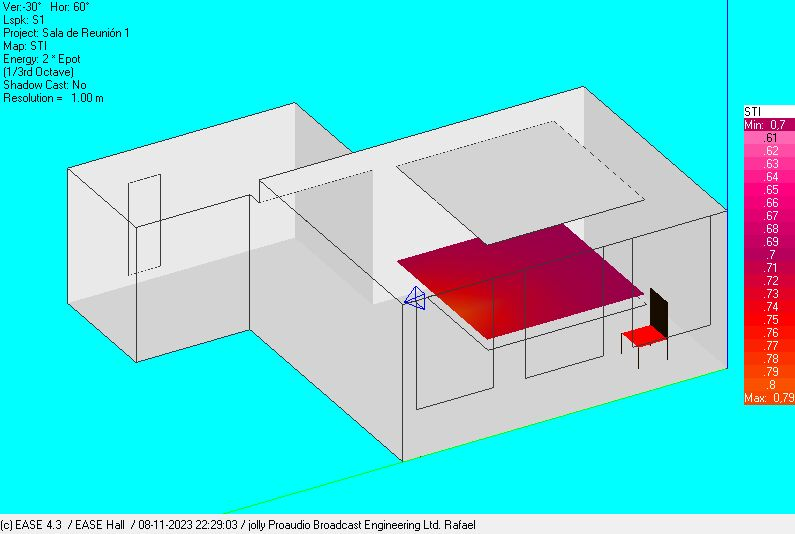
\includegraphics[width=8cm]{images/STI acondicionado/STI_Reunion1_ConAcond.jpg}
        \caption{STI de sala de reunión 1 acondicionado}
        \label{fig:STI sala 1 acond}
    \end{figure}
\end{frame}

\begin{frame}{Resultados salas de reuniones}
    \begin{figure}
        \centering
        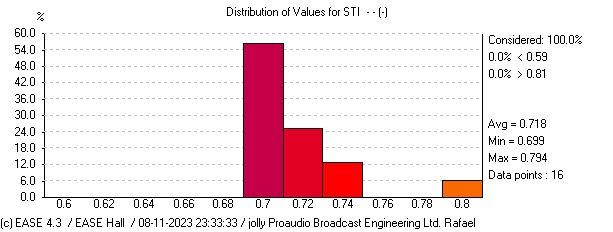
\includegraphics[width=8cm]{images/STI acondicionado/STIdist_Reunion1_ConAcond.jpg}
        \caption{Distribución STI de sala de reunión 1 acondicionado}
        \label{fig:dis STI sala 1 acond}
    \end{figure}
\end{frame}

\begin{frame}{Resultados salas de reuniones}
    \begin{figure}
        \centering
        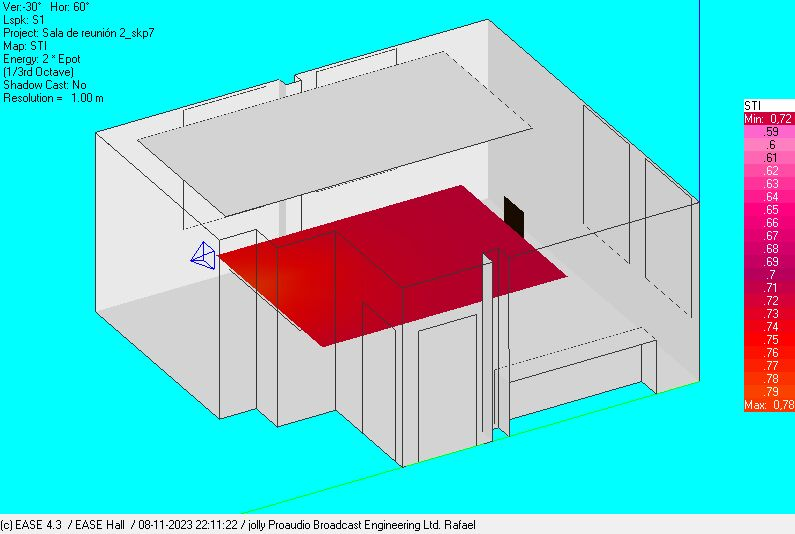
\includegraphics[width=8cm]{images/STI acondicionado/STI_Reunion2_ConAcond.jpg}
        \caption{STI de sala de reunión 2 acondicionado}
        \label{fig:STI sala 2 acond}
    \end{figure}
\end{frame}

\begin{frame}{Resultados salas de reuniones}
    \begin{figure}
        \centering
        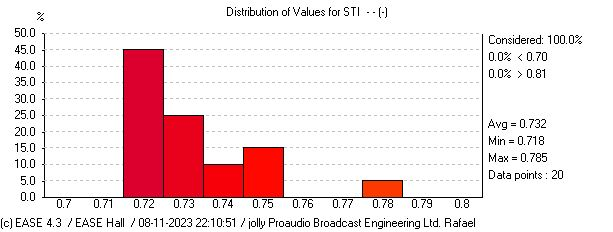
\includegraphics[width=8cm]{images/STI acondicionado/STIdist_Reunion2_ConAcond.jpg}
        \caption{Distribución STI de sala de reunión 2 acondicionado}
        \label{fig:dist STI sala 2 acond}
    \end{figure}
\end{frame}

\begin{frame}{Resultados salas de reuniones}
    \begin{table}[H]
        \centering
        \caption{Parámetros acústicos de las salas de reunión del estado actual y acondicionado}
        \label{tab: resultados salas de reunion}
        \resizebox{\textwidth}{!}{%
        \begin{tabular}{|l|l|ll|ll|}
        \hline
         &  & \multicolumn{2}{l|}{\textbf{Sala de reunión 1}} & \multicolumn{2}{l|}{\textbf{Sala de reunión 2}} \\ \cline{3-6} 
        \multirow{-2}{*}{\textbf{Parámetro}} & \multirow{-2}{*}{\textbf{Recomendación}} & \multicolumn{1}{l|}{\textbf{Estado actual}} & \textbf{Propuesta} & \multicolumn{1}{l|}{\textbf{Estado actual}} & \textbf{Propuesta} \\ \hline
        $T_{target}$ & 0.6 & \multicolumn{1}{l|}{\textcolor{red}{No cumple}} & \textcolor{teal}{Cumple} & \multicolumn{1}{l|}{\textcolor{red}{No cumple}} & \textcolor{teal}{Cumple} \\ \hline
        $C_{50speech}$ & $C_{50speech}>0$ & \multicolumn{1}{l|}{\textcolor{teal}{1.79}} & \textcolor{teal}{3.5} & \multicolumn{1}{l|}{\textcolor{teal}{0.89}} & \textcolor{teal}{3.9} \\ \hline
        STI & STI \textgreater 0.45 & \multicolumn{1}{l|}{\textcolor{teal}{0.66}} & \textcolor{teal}{0.70} & \multicolumn{1}{l|}{\textcolor{teal}{0.64}} & \textcolor{teal}{0.72} \\ \hline
        \end{tabular}%
        }
    \end{table}
\end{frame}
\begin{frame}{Resultados sala de ensayo}
    \begin{figure}[H]
        \centering
        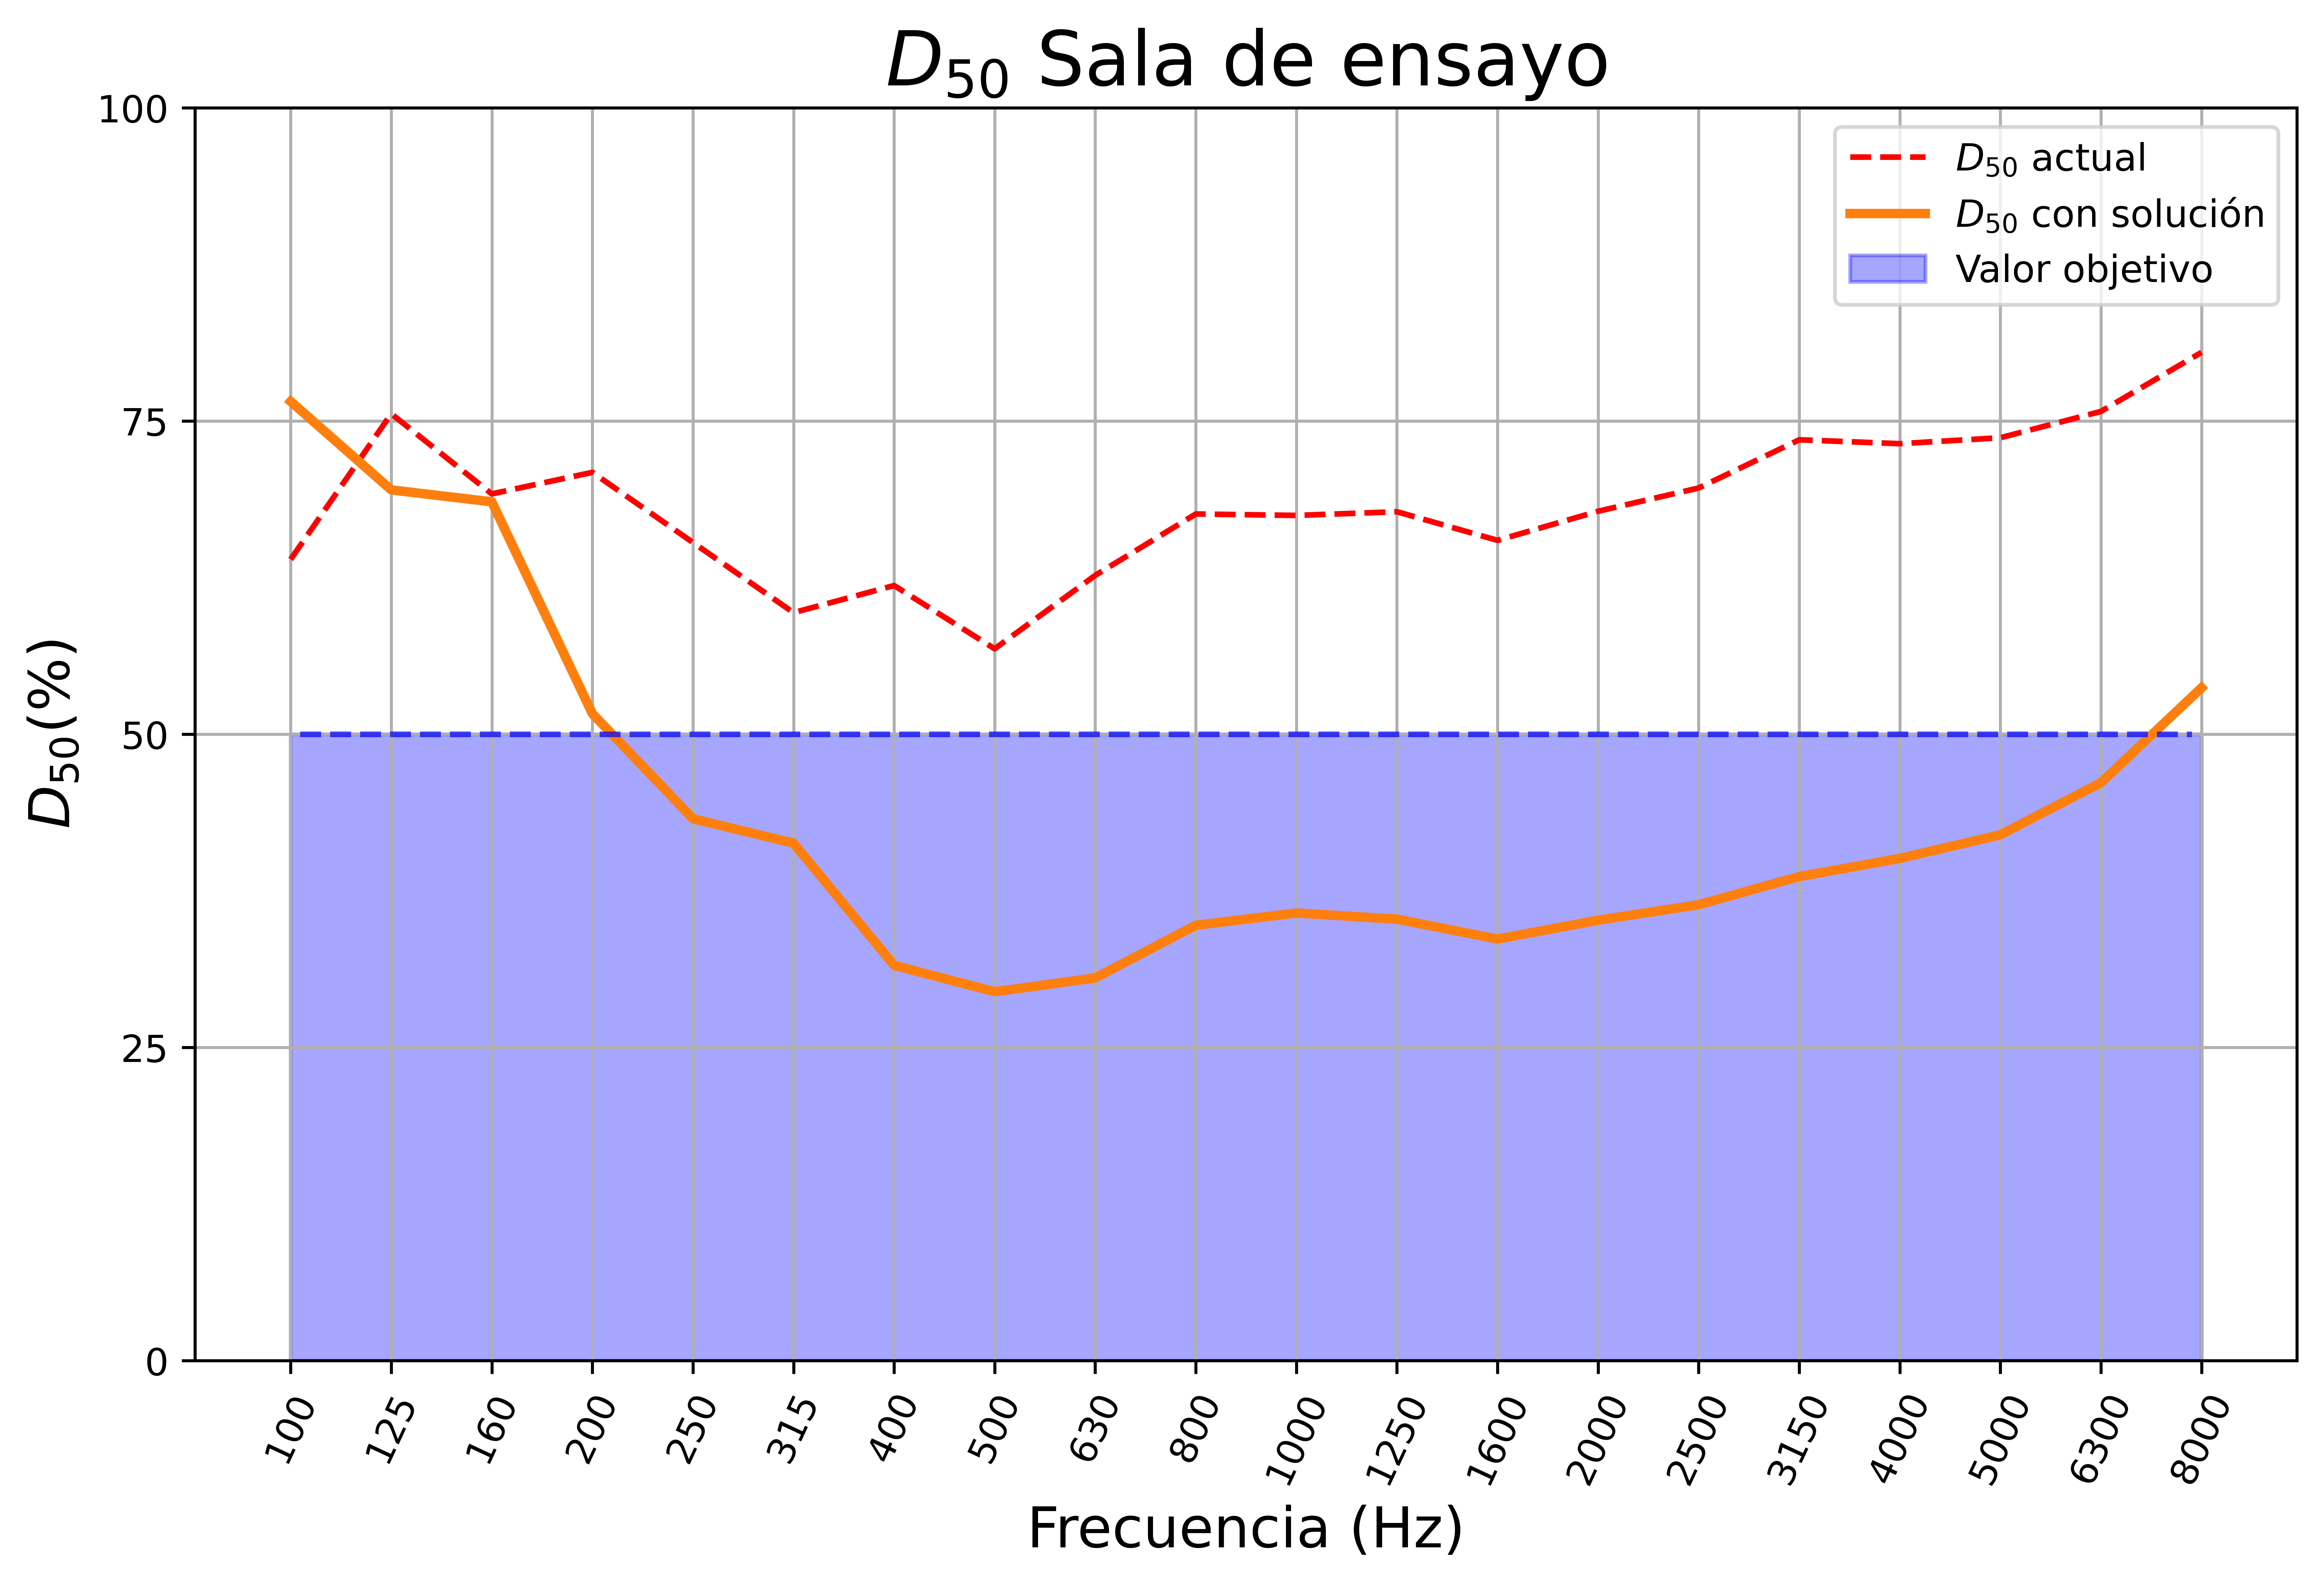
\includegraphics[width=8cm]{images/D50_comparacion.png}
        \caption{Comparación de D50 en sala de ensayo en su estado actual y acondicionado}
    \end{figure}
\end{frame}

\begin{frame}{Resultados sala de ensayo}
   
\begin{table}[H]
    \centering
    \caption{Parámetros acústicos de la sala de ensayo del estado actual y acondicionado}
    \label{tab: resultados sala de ensayo}
    \begin{tabular}{|l|l|ll|}
    \hline
     &  & \multicolumn{2}{l|}{\textbf{Sala de ensayo}} \\ \cline{3-4} 
    \multirow{-2}{*}{\textbf{Parámetro}} & \multirow{-2}{*}{\textbf{Recomendación}} & \multicolumn{1}{l|}{\textbf{Estado actual}} & \textbf{Propuesta} \\ \hline
    $RT_{mid}$ & 0.3 - 0.7 & \multicolumn{1}{l|}{\textcolor{red}{0.74}} & \textcolor{teal}{1.4} \\ \hline
    $C_{80}$ & $-2<C_{80}<2$ & \multicolumn{1}{l|}{\textcolor{red}{6.04}} & \textcolor{teal}{3} \\ \hline
    $D_{50}$ & $D_{50}$ \textless 0.5 & \multicolumn{1}{l|}{\textcolor{red}{$65\%$}} & \textcolor{teal}{$33\%$} \\ \hline
    \end{tabular}
\end{table}
\end{frame}


\section{Presupuesto}
\begin{frame}{Presupuesto del proyecto}
    El presupuesto esta desglosado en la siguiente tabla por cada actividad propuesta en la carta Gantt antes presentada.
\begin{figure}[H]
    \centering
    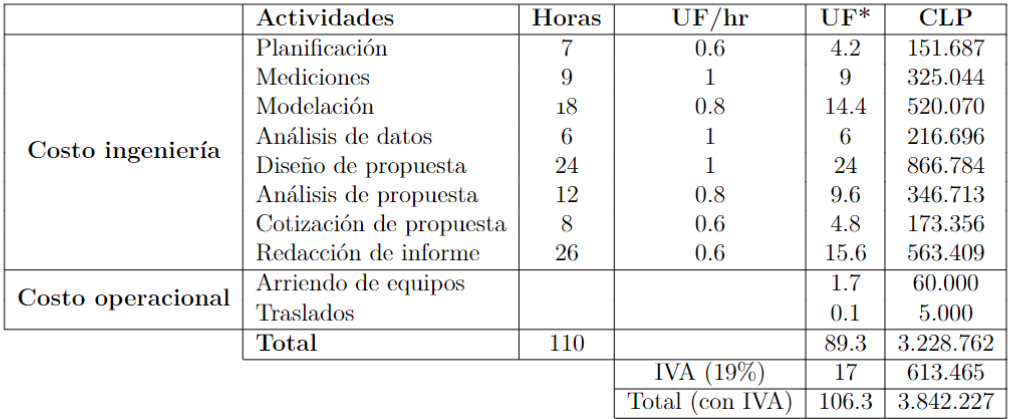
\includegraphics[width=10cm]{images/Presupuesto.png}
    \caption{Presupuesto del proyecto}
    \label{fig:presupuesto}
\end{figure}    
\end{frame}

\begin{frame}{Presupuesto de materiales}
    %añadir imagen con tabla
\end{frame}

\section{Medición coeficiente de absorción acústica de un material}
\begin{frame}{Materiales escogidos}
    Se escogió un panel de madera ranurado de 2.4 cm de espesor, con lana de vidrio y lana mineral, midiéndolo sin plenum y plenum de 2 cm.
    \begin{figure}[H]
        \centering
        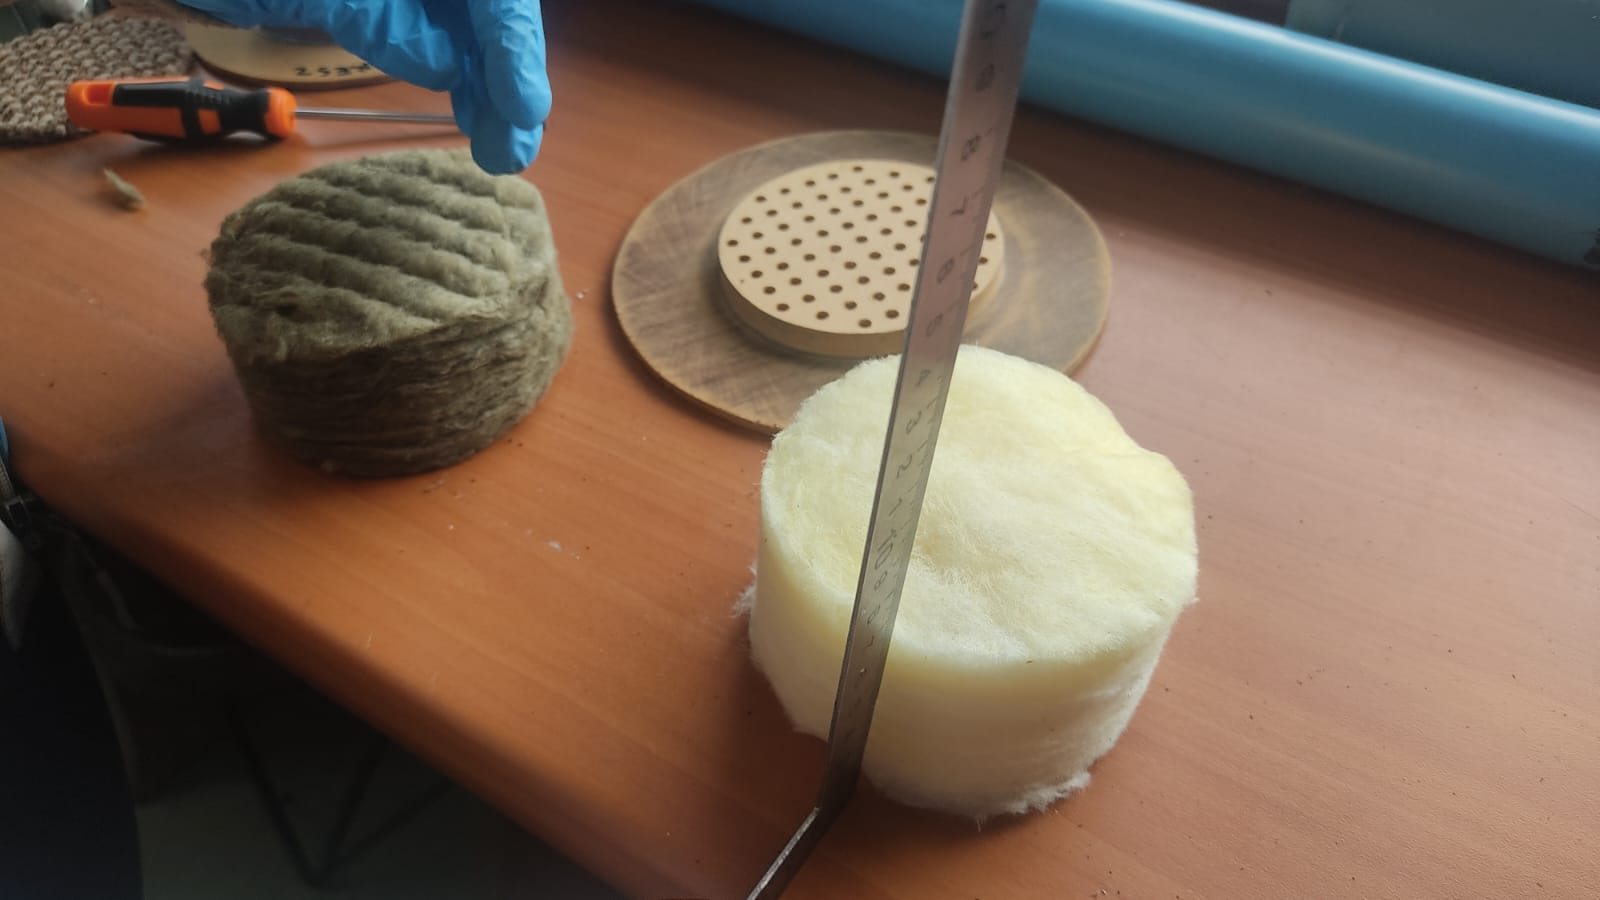
\includegraphics[width=7cm]{images/Medición abs/materiales.jpeg}
        \caption{Materiales de medición}
        \label{fig: materiales a medir}
    \end{figure}
\end{frame}

\begin{frame}{Madera ranurada}
    \begin{figure}[H]
        \centering
        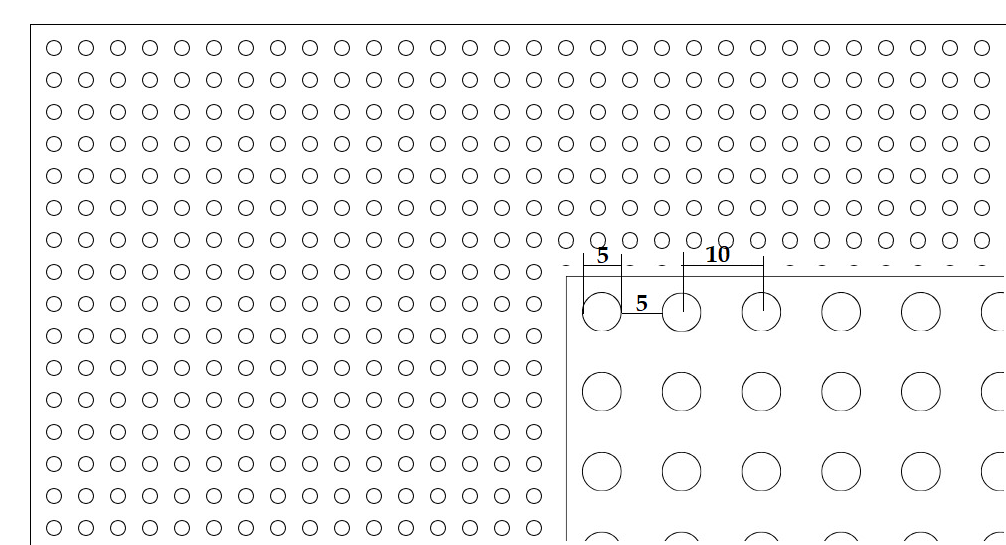
\includegraphics[width=7cm]{images/Medición abs/MATERIAL.png}
        \caption{Dimensiones de madera ranurada}
        \label{fig: madera ranurada}
    \end{figure}
\end{frame}

\begin{frame}{Materiales escogidos}
    \begin{figure}
        \centering
        \includegraphics[width=9cm]{images/Medición abs/Tabla coef.png}
        \caption{Valores de coeficiente de absorción}
        \label{fig:enter-label}
    \end{figure}
\end{frame}

\begin{frame}{Resultados}
    \begin{figure}
        \centering
        \includegraphics[width=9cm]{images/Medición abs/Grafico coef.abs LanaMineral.png}
        \caption{Coeficiente de absorción de lana mineral}
        \label{fig:grafico coef Lana mineral}
    \end{figure}
\end{frame}

\begin{frame}{Resultados}
    \begin{figure}
        \centering
        \includegraphics[width=9cm]{images/Medición abs/Grafico coef.abs LanaVidrio.png}
        \caption{Coeficiente de absorción de lana de vidrio}
        \label{fig:grafico coef Lana vidrio}
    \end{figure}
\end{frame}

\section{Conclusiones}
\begin{frame}{Conclusiones}
    \begin{itemize}
        \item Se logró cumplir con las actividades propuestas en el cronograma.
        \item A raíz de los resultados de las mediciones, se logró identificar si estos son adecuados acústicamente para el uso de cada uno de estos recintos.
        \item El ruido presente en los salones es el problema que predomina, incumpliendo con las curvas NC recomendadas para su uso.
        \item En el caso del tiempo de reverberación en las salas de reuniones según la norma DIN18041 estos no cumplen con valores acordes a su uso. Lo cual con la propuesta dada en este proyecto se logró cumplir con este criterio, además de mejorar la claridad y la inteligibilidad de la palabra en ambas salas.
        \item En el caso del tiempo de reverberación de la sala de ensayo, los valores eran demasiado bajos con la implementación que se realizó por parte de la administración.
    \end{itemize}
\end{frame}

\footlinecolor{sintefblue}

\backmatter

\end{document}
